% LaTeX path to the root directory of the current project
\providecommand{\econtexRoot}{}
\renewcommand{\econtexRoot}{.}
\providecommand{\econtex}{\econtexRoot/texmf-local/tex/latex/econtex}
\providecommand{\econtexSetup}{\econtexRoot/texmf-local/tex/latex/econtexSetup}
\providecommand{\econtexShortcuts}{\econtexRoot/texmf-local/tex/latex/econtexShortcuts}
\providecommand{\econtexBibMake}{\econtexRoot/texmf-local/tex/latex/econtexBibMake}
\providecommand{\econtexBibStyle}{\econtexRoot/texmf-local/bibtex/bst/econtex}
\providecommand{\notes}{\econtexRoot/texmf-local/tex/latex/handout}
\providecommand{\handoutSetup}{\econtexRoot/texmf-local/tex/latex/handoutSetup}
\providecommand{\handoutShortcuts}{\econtexRoot/texmf-local/tex/latex/handoutShortcuts}
\providecommand{\handoutBibMake}{\econtexRoot/texmf-local/tex/latex/handoutBibMake}
\providecommand{\handoutBibStyle}{\econtexRoot/texmf-local/bibtex/bst/handout}

  

\documentclass[titlepage]{\econtex}
\providecommand{\texname}{LiqConstr}% Keyname for the bibtex entry corresponding to this paper
\usepackage{vmargin} %%% Private
\usepackage{\econtexSetup}\usepackage{\econtexShortcuts}

\provideboolean{ifWeb} 
\setboolean{ifWeb}{false}
\opt{Web}{\setboolean{ifWeb}{true}}

\ifthenelse{\boolean{ifWeb}}{\usepackage{grfext}
\PrependGraphicsExtensions*{.svg,.jpg,.JPG,.png,.PNG,.pdf,.PDF}
}{}


%%% Private: The stuff below switches on and off the creation of the files in the "Sections" subdirectory
%%% Sections was useful when constructing the paper so that individual parts could be edited independently
%%% It is now a legacy and is preserved mainly as a template for how to do this for future projects
\newboolean{verbatimwriteOn}        %%% Private
\setboolean{verbatimwriteOn}{true}  %%% Private
\setboolean{verbatimwriteOn}{false} %%% Private
\newcommand{\ifVerbatimWrite}{\ifthenelse{\boolean{verbatimwriteOn}}} %%% Private
\ifVerbatimWrite{}{ %%% Private 
  \renewenvironment{verbatimwrite}[1]{} %%% Private 
} %%% Private

\newenvironment{Private}{} %%% Private 

\providecommand{\wAlt}{\omega}
\providecommand{\sConst}{\varsigma}

\newboolean{Figures}
\setboolean{Figures}{true}

\newboolean{FigFileNames}
\setboolean{FigFileNames}{true}

\newboolean{StandAlone}
\setboolean{StandAlone}{false}

\newtheorem{defn}{Definition}
\newtheorem{theorem}{Theorem}
\newtheorem{lemma}{Lemma}
\newtheorem{corollary}{Corollary}
\newtheorem{prop}{Proposition}

\usepackage{datetime}

\renewcommand{\cite}{\citeyear}

\setmarginsrb{1in}{1in}{1in}{1.4in}{0pt}{0pt}{0pt}{.3in} %%% Private : Large font for easy viewing and editing on small screen 
% {left}{top}{right}{bottom} %%% Private

\provideboolean{bigdouble}    %%% Private : Large font for easy viewing and editing on small screen
\setboolean{bigdouble}{true}  %%% Private : Large font for easy viewing and editing on small screen
\setboolean{bigdouble}{false} %%% Private : Large font for easy viewing and editing on small screen

\ifthenelse{\boolean{bigdouble}}{ % Margins must be set before begin document command  %%% Private : Large font for easy viewing and editing on small screen
  \setmarginsrb{0.40in}{0.8in}{0.40in}{0.8in}{0pt}{0pt}{0pt}{0.2in} %%% Private : Large font for easy viewing and editing on small screen
  % {left}{top}{right}{bottom} %%% Private : Large font for easy viewing and editing on small screen
}{} %%% Private : Large font for easy viewing and editing on small screen

\begin{document}\bibliographystyle{\econtexBibStyle}

\hfill{\tiny \texname}

\title{Liquidity Constraints \\ and Precautionary Saving}

\newlength\TableWidth

\ifthenelse{\boolean{ifWeb}}{
\author{
  Christopher D. Carroll\authNum
  \and
  Martin B. Holm\authNum
  \and
  Miles S. Kimball\authNum
}
}{
\author{
  Christopher D. Carroll\authNum \\ {\small JHU}
  \and
  Martin B. Holm\authNum \\ {\small University of Oslo} 
  \and
  Miles S. Kimball\authNum \\ University of Colorado at Boulder
}
} % End ifWeb

\date{January 22, 2019}
\maketitle

\jelclass{C6, D91, E21}

\keywords{liquidity constraints, uncertainty, precautionary saving}


\hypertarget{Abstract}{}
\begin{abstract}
    \begin{verbatimwrite}{./\texname-abstract.metadata} %%% Private
      Economists working with numerical solutions to the optimal consumption/saving problem have long known that there are quantitatively important interactions between liquidity constraints and precautionary saving behavior.  This paper provides the analytical basis for those interactions.  We first explain why the introduction of a liquidity constraint increases the precautionary saving motive. We then provide a rigorous basis for the oft-noted similarity between the effects of introducing uncertainty and introducing constraints: In both cases the effects spring from the concavity in the consumption function which either uncertainty or constraints can induce.  We further show that consumption function concavity, once created, propagates back to consumption functions in prior periods.  Finally, our most surprising result is that the introduction of additional constraints beyond the first one or the introduction of additional risks beyond a first risk can actually reduce the precautionary saving motive -- the new constraint or risk can `hide' the effects of pre-existing constraints or risks.
  \end{verbatimwrite}\ifVerbatimWrite{\input{./\texname-abstract.metadata}}{} %%% Private
\end{abstract}


\ifthenelse{\boolean{ifWeb}}{}{\begin{small}}
\parbox{\textwidth}{
  \begin{center}
\begin{tabbing}
  \texttt{Econ-ARK:~} \= \= \url{http://econ.jhu.edu/people/ccarroll/papers/LiqConstr.pdf} \kill \\  % This line establishes the locations of the tabs, but is not printed because of the \kill directive
\texttt{~~~~Repo:~} \= \= \url{https://github.com/llorracc/LiqConstr}  \\
\texttt{~~~~~PDF:~} \> \> \url{http://econ.jhu.edu/people/ccarroll/papers/LiqConstr.pdf} \\
\texttt{~~~~~Web:~} \> \> \url{http://econ.jhu.edu/people/ccarroll/papers/LiqConstr/} \\
%\texttt{~BibTeX:~} \> \> \url{http://econ.jhu.edu/people/ccarroll/papers/LiqConstr.bib} \\
%\texttt{Archive:~} \> \> \url{http://econ.jhu.edu/people/ccarroll/papers/LiqConstr.zip} \\
\texttt{~~Slides:~} \> \> \href{http://econ.jhu.edu/people/ccarroll/papers/LiqConstr-Slides.pdf}{http://econ.jhu.edu/people/ccarroll/papers/LiqConstr-Slides.pdf} \\
\texttt{Econ-ARK:} \> \> \url{http://github.com/Econ-ARK/REMARK/tree/master/REMARKs/LiqConstr.md} \\
\end{tabbing}
\end{center}
}
\ifthenelse{\boolean{ifWeb}}{}{\end{small}}

\hypersetup{pdfauthor={Christopher Carroll <ccarroll@jhu.edu>, Martin Holm <martin.b.holm@outlook.com>, Miles Kimball <miles.kimball@colorado.edu>},
            pdftitle={Liquidity Constraints and Precautionary Saving},
            pdfsubject={Liquidity Constraints and Precautionary Saving},
            pdfkeywords={liquidity constraints, consumption function, uncertainty, precautionary saving},
            pdfproducer = {LaTeX with hyperref},
            pdfcreator = {pdflatex}
            }

\begin{authorsinfo}
  \name{Carroll: Department of Economics, Johns Hopkins University, \url{http://econ.jhu.edu/people/ccarroll/}, \href{mailto:ccarroll@jhu.edu}{\texttt{ccarroll@jhu.edu}}}
\name{Holm: Department of Economics, University of Oslo, \href{mailto:martin.b.holm@outlook.com}{\texttt{martin.b.holm@outlook.com}}}
\name{Kimball: \url{https://www.colorado.edu/economics/people/faculty/miles-spencer-kimball}, \href{mailto:miles.kimball@colorado.edu}{\texttt{miles.kimball@colorado.edu}}}
\end{authorsinfo}

\thanks{This paper supersedes NBER working paper no.\ 8496 from 2001. We are grateful to Luigi Pistaferri, Misuka Otsuka, and to conference participants in the conferences ``Macroeconomics and Household Borrowing'' sponsored by the Finance and Consumption program and the European University in May 2005 and ``Household Choice of Consumption, Housing, and Portfolio'' at CAM in Copenhagen in June 2005. Kimball is grateful to the National Institute on Aging for research support via grant P01-AG10179.
  \\ 
We are grateful to Mark Huggett for suggesting the current proof one of our lemmas, which was a substantial improvement over our original proof, to Luigi Pistaferri for an insightful discussion of the paper, to conference participants at the ``International Savings and Pensions Conference'' in Venice in 1999; to Misuzu Otsuka for meticulous proofreading and mathematical checking; and to participants in the conferences ``Macroeconomics and Household Borrowing'' sponsored by the Finance and Consumption program and the European University in May 2005, and ``Household Choice of Consumption, Housing, and Portfolio'' at CAM in Copenhagen in June 2005.  Kimball is grateful to the National Institute on Aging for research support via grant P01-AG10179.}

\titlepagefinish
\setcounter{page}{1}

\setcounter{footnote}{0}


\hypertarget{Introduction}{}
\section{Introduction}\label{sec:Intro}
\ifthenelse{\boolean{bigdouble}}{\large}{} %%% Private

\begin{verbatimwrite}{./Sections/Intro.tex} %%% Private

Numerical solutions have supplanted analytical methods for theoretical modeling of consumption/saving choices because analytical solutions are not available for realistic descriptions of utility and uncertainty.

But a drawback to numerical solutions is that it is often difficult to know why results come out the way they do.  A leading example is in the relationship between precautionary saving behavior and liquidity constraints.  At least since \citet{zeldes:thesis}, economists working with numerical solutions have known that liquidity constraints can strictly increase precautionary saving under very general circumstances - even for consumers with a quadratic utility function that generates no intrinsic precautionary saving motive.\footnote{For the seminal numerical examination of some of the interactions between precautionary saving and liquidity constraints, see \citet{deatonLiqConstr}, who also provides conditions under which the problem defines a contraction mapping.} On the other hand, simulation results have sometimes seemed to suggest that liquidity constraints and precautionary saving are substitutes rather than complements.  In an early example, \citet{samwick:pensions} showed that unconstrained consumers with a precautionary saving motive in a retirement saving model behave in ways qualitatively and quantitatively similar to the behavior of liquidity constrained consumers facing no uncertainty.

This paper provides the theoretical tools needed to make sense of the interactions between liquidity constraints and precautionary saving. These tools provide a rigorous theoretical foundation that can be used to clarify the reasons for the numerical literature's apparently contrasting findings.

For example, one of the paper's simpler points is a proof that when a liquidity constraint is added to the standard consumption problem, the resulting value function exhibits increased prudence around the level of wealth where the constraint becomes binding.\footnote{\citet{kimball:smallandlarge} defines prudence of the value function and shows that it is the key theoretical requirement to produce precautionary saving.}  % The essential logic for why a liquidity constraint can induce precautionary saving is relatively straightforward.
Constraints induce precaution because constrained agents have less flexibility in responding to shocks when the effects of the shocks cannot be spread out over time. The precautionary saving motive is heightened by the desire (in the face of risk) to make such constraints less likely to bind.

At a deeper level, we show that the effect of a constraint on prudence is an example of a general theoretical result: Prudence is induced by concavity of the consumption function. Since a constraint causes consumption concavity around the point where the constraint binds,\footnote{Since the first version of this paper, the connection between constraints and consumption concavity has been explored in more specific settings (see e.g. \citet{park2006analytical} for CRRA utility,  \citet{nishiyama2012concavity} for quadratic utility, and \citet{holm2018consumption} for the case with infinitely-lived households with HARA utility).} adding a constraint necessarily boosts prudence around that point. We show that this concavity-boosts-prudence result holds for any utility function with non-negative third derivative; ``prudence'' in the utility function \cite{kimball:smallandlarge} is not necessary, because prudence is created by consumption concavity.

These results connect closely to \citet{carroll&kimball:concavity}'s demonstration that, within the HARA class, the introduction of uncertainty causes the consumption function to become strictly concave (in the absence of constraints) for all but a few knife-edge combinations of utility function and uncertainty.  Taken together, the two papers can be seen as establishing rigorously the sense in which precautionary saving and liquidity  constraints are substitutes.\footnote{See \citet{fernandez-corugedo:softlc} for a related demonstration that `soft' liquidity constraints bear an even closer resemblance to precautionary behavior. \citet{MendelsonAmihud:consumption} provide an impressive treatment of a similar problem.} To illustrate this point, in appendix \ref{app:similar} we provide an example of a specific kind of uncertainty that (under CRRA utility, in the limit) induces a consumption function that is point-wise identical to the consumption function that would be induced by the addition of a liquidity constraint.

We further show that, once consumption concavity is created (by the introduction of either uncertainty or a constraint), it propagates back to periods before the period in which the concavity has been introduced.\footnote{\citet{carroll&kimball:concavity} showed that the concavity induced by uncertainty propagated backwards, but the proofs in that paper cannot be applied to concavity created by a liquidity constraint.} %But in the quadratic utility case the propagation is rather subtle: the prior-period consumption rules are concave (and prudence is higher) at any level of wealth from which it is possible that the constraint will bind, but also possible that it may not bind.  Precautionary saving takes place in such circumstances because a bit more saving can reduce the probability that the constraint will bind.
Precautionary saving arises from the \textit{possibility} that constraints might bind; this may help to explain why such a high percentage of households cite precautionary motives as the most important reason for saving \citep{kennickell&lusardi:scfquestions} even though the fraction of households who report actually having been constrained in the past is relatively low \citep{jappelli:whoisconstr}.


Our final theoretical contribution is to show that the introduction of further liquidity constraints beyond the first one may actually \textit{reduce} precautionary saving at some levels of wealth by `hiding' the effects of the pre-existing constraint(s). Identical logic implies that uncertainty can hide the effects of a constraint, because the consumer may save so much for precautionary reasons that the constraint becomes irrelevant.  For example, a typical perfect foresight model of retirement consumption for a consumer with Social Security income implies that the legal constraint on borrowing against Social Security benefits will cause the consumer to run assets down to zero, then set consumption equal to income for the remainder of life.  Now consider adding the possibility of large medical expenses near the end of life (e.g.\ nursing home fees; see \cite{aclvJoy}).  Under reasonable assumptions, a consumer facing such a risk may save enough for precautionary reasons to render the constraint irrelevant.

The rest of the paper is structured as follows.  To fix notation and ideas, the next section sets out our general theoretical framework. The third section shows that concavity of the consumption function heightens prudence.  The fourth section shows how concavity, whether induced by constraints or uncertainty, propagates to previous periods. Section 5 shows how the introduction of a constraint creates a precautionary saving motive. The sixth section shows when the introduction of additional liquidity constraints beyond the first constraint increases the precautionary motive at any given level of wealth.  The fact that this does not always occur means that the introduction of constraints or uncertainty can hide the effects of pre-existing constraints or uncertainty. The final section concludes.

\end{verbatimwrite}\ifVerbatimWrite{\input{./Sections/Intro.tex}}{} %%% Private

\section{The Setup}\label{sec:Setup}
%\subfile{Sections/Setup}
\begin{verbatimwrite}{Sections/Setup} %%% Private
  
  In this section, we lay out the basic setup of the consumption/saving problem with many periods. Consider a consumer who faces some future risks but is not subject to any current or future liquidity constraints.  The consumer is maximizing the time-additive present discounted value of utility from consumption $u(c)$.  With interest and time preference factors $R \in (0,\infty)$ and $\beta \in (0,\infty)$, respectively, and labeling consumption $c$, stochastic labor income $y$, and gross wealth (inclusive of period-t labor income) $w_{t}$, the consumer's problem can be written as%\footnote{%We allow for a stochastic discount factor because some problems which contain a stochastic scaling variable (such as permanent income) can be analyzed more easily by dividing the problem through by the scale variable; this division induces a term that effectively plays the role of a stochastic discount factor.}
\begin{eqnarray*}
V_{t}(w_{t}) &=&
%\max_{\{c_{t}\}}~u(c_{t})+\Ex_{t}\left[\sum_{s=t+1}^{T}\left(\prod_{j=t+1}^{s}\tilde{\beta}_{j}\right) u(\tilde{c}_{s})\right]
                 \max_{c} \Ex_{t}\left[\sum_{k=0}^{T-t}\beta^{k} u({c_{t+k}})\right]   \label{eq:valuefn} \\
   & s.t. &  \nonumber
\\              w_{t+1} & = & R(w_{t}-c_{t})+y_{t+1}.
\nonumber
\end{eqnarray*}
where in some (but not all) of our results we consider utility functions of the HARA class
\begin{equation}\label{eq:HARA}
  u(c) = \begin{cases} \frac{1}{a - 1}\left(ac + b\right)^{\frac{a-1}{a}} & a \neq 0,1 \\
-be^{-c/b} & a = 0 \\
\log(c + b) & a = 1 \end{cases} \end{equation}
with $b > \max\{- ac,0\}$. Note that that \eqref{eq:HARA} nests the case with quadratic utility ($a = -1$).\footnote{$u'(c)>0$ and $u''(c) < 0$ is holds for all utility functions in this class.}

As usual, the recursive nature of the problem makes this equivalent to the Bellman equation:
\begin{eqnarray*}  \label{eq:recursiveV}
V_{t}(w_{t}) & = & \max_{c} ~ u(c) + \Ex_{t} [{\beta}
V_{t+1}(%
{R}(w_t - c) + {y}_{t+1})].
\end{eqnarray*}
We define
\begin{equation*} \label{eq:OmegaEV}
\Omega_t(s_t) = \Ex_t [ \beta V_{t+1}(R s_t + y_{t+1})]
\end{equation*}
as the end-of-period value function where $s_t = w_t - c_t$ is the portion of period t resources saved. We can then rewrite the problem as\footnote{For notational simplicity we express the value function $V_t(w)$ and the expected discounted value function $\Omega_{t}(s)$ as functions simply of wealth and savings, but implicitly these functions reflect the entire information set as of time t; if, for example, the income process is not i.i.d., then information on lagged income or income shocks could be important in determining current optimal consumption.  In the remainder of the paper the dependence of functions on the entire information set as of time $t$ will be unobtrusively indicated, as here, by the presence of the $t$ subscript. For example, we will call the policy rule in period $t$ which indicates the optimal value of consumption $c_{t}(w)$. In contrast, because we assume that the utility function is the same from period to period, the utility function has no $t$ subscript.}
\begin{eqnarray*}  \label{eq:subphi}
V_{t}(w_{t}) & = & \max_{c} ~ u(c) + \Omega_{t}(w_t - c).
\end{eqnarray*}
Throughout the paper, we distinguish between two different consumption functions, $c_t(w)$ and $\chi_t(s)$. $c_t(w)$ is the beginning-of-period consumption function and implicitly defined by the envelope conditions with respect to the current value function: $u'(c_t(w)) = V'(w)$. $\chi_t(s)$ is the end-of-period consumption function implicitly defined by the envelope condition with respect to expected value: $u'(\chi_t(s)) = \Omega_{t}'(s)$.

\end{verbatimwrite}\ifVerbatimWrite{\begin{align}
\max \quad E_t \Sigma_{n=0}^{T-t} \beta^{n}u(c_{t+n})
\end{align}

\begin{align} \text{s.t.} \quad b_{t+1} &= R[b_t + y_t - c_t]\\
y_t &= p_tv_t\\
p_t &= G_tp_{t-1}n_t 
\end{align}

\bigskip

$y$: current labor income \\

$p$: permanent labor income \\

$v$: transitory income shock \\

$n$: permanent income shock \\

$G = (1+g)$: growth factor for permanent labor income \\

$b$: stock of physical net wealth \\

$R = (1+r)$: gross interest rate \\

$\beta = 1/(1+\delta)$: discount factor \\}{} %%% Private

\hypertarget{PrudAndCC}{}
\section{Consumption Concavity and Prudence}\label{sec:PrudAndCC}

\begin{verbatimwrite}{Sections/PrudAndCC} %%% Private

Our ultimate goal is to understand the relationship between liquidity
constraints and precautionary saving. There are three steps: consumption concavity increases prudence (Section \ref{sec:PrudAndCC}), liquidity constraints cause consumption concavity (Section \ref{sec:Precaution}), and prudence affects precautionary saving (Section \ref{sec:ConstrRisksCPPandPS}).

Our analysis of consumption concavity and prudence in this section is couched in general terms and therefore applies whether the source of concavity is liquidity constraints or something else (e.g., uncertainty).  %Our treatment here will therefore alternate between a discussion of the effects of imposing liquidity constraints and the effects of introducing uncertainty.
%We start by defining consumption concavity and counterclockwise concavification before we proceed to show the relationship between consumption concavity and prudence.

\begin{Private}\begin{comment} % This subsection is not necessary with the new material on piecewise linearity
\subsection{When Is the Consumption Function Linear?}\label{subsec:WhenLin}

Carroll and Kimball~\cite{carroll&kimball:concavity} prove that for
utility functions in the HARA class, in the absence of liquidity
constraints the consumption function will be linear ($c''_{t}(w_{t}) =
0$) only in three cases: when utility is of the Constant Relative Risk
Aversion (CRRA) form $u(c) = c^{1-\gamma}/(1-\gamma)$ and the only
future risk is multiplicative (i.e.  rate-of-return
risk);\footnote{The consumption function when utility is CRRA with a
shifted origin, $u(c)=(c-\kappa)^{1-\gamma}/(1-\gamma)$, is \textit{not}
linear when there is multiplicative risk, as can be seen from the
first order condition for the penultimate period of life when
$\beta=1$:
$(c_{T-1}-\kappa)^{-\gamma}=\Ex_{T-1}[(\tilde{R}_{T}(w_{T-1}-c_{T-1})-\kappa)^{-\gamma}]$
implying that $c_{T-1}-\kappa =
\{\Ex_{T-1}[(\tilde{R}_{T}(w_{T-1}-c_{T-1})-\kappa)^{-\gamma}]\}^{-1/\gamma}$
which has no linear solution for $c_{T-1}$ unless $\kappa=0$.} when
utility is of the Constant Absolute Risk Aversion (CARA) form $u(c) =
-(1/a) e^{-a c}$ and the only future risk is additive (i.e.  labor
income risk); and when the utility function is quadratic, $u(c) =
-(\alpha/2)(c-\kappa)^{2}$.\footnote{See section
\ref{subsubsec:QuadCase} for a demonstration that the consumption
rule is linear under quadratic utility in the presence of both labor
income and rate-of-return risk.} Thus, the natural baseline cases to
consider are the three HARA cases where the consumption function is
linear.
\end{comment}
\end{Private}

%%%\subsection{How Does Consumption Concavity Heighten
%%%  Prudence?} \label{subsec:CCToPrud}
%%%\ifthenelse{\boolean{Outline}}{ %\ref{subsec:DefHARACCPrud}
%%%\immediate{\write18{echo "-"  CCToPrud >> ./Index.txt}}}{}


\subsection{Definitions}
%%%We first need to define two concepts: consumption concavity and counterclockwise concavification.
%%%We will be working with a specific version of utility functions, the hyperbolic absolute risk avesion (HARA) class.
%%%\begin{defn}(HARA utility). \\
%%%	A utility function is of the HARA class if
%%%	\begin{equation} \label{eq:HARA}
%%%	u(c) = \begin{cases} \frac{1}{a-1}(ac + b)^{1-\frac{1}{a}} & \text{ if $a \neq 0$ and $a \neq 1$}\\
%%%	- b e^{-c/b} & \text{ if $a = 0$}\\
%%%	\log(c+b) & \text{ if $a = 1$}
%%%	\end{cases}
%%%	\end{equation}
%%%	and $b \geq - ac$.
%%%\end{defn}
%%%\noindent Note that $u' > 0$ and $u'' \leq 0$ for all HARA utility functions.
%%%
%%%Marginal utility of the HARA utility is
%%%\begin{equation}
%%%u'(c) = \begin{cases} (ac + b)^{-\frac{1}{a}} & \text{ if $a \neq 0$}\\
%%%e^{-c/b} & \text{ if $a = 0$}
%%%\end{cases}
%%%\end{equation}
%%%where we observe that HARA utility contains the cases with CRRA utility ($a > 0, b = 0$), CARA ($a = 0, b> 0$), and quadratic ($a = -1, b > 0$).
%%%\subsubsection{Definition of HARA Utility}\label{subsubsec:DefHARA}
%%%\ifthenelse{\boolean{Outline}}{ %\ref{subsec:DefHARACCPrud}
%%%\immediate{\write18{echo "...."  DefHARA >> ./Index.txt}}}{}
%%% SUGGESTION FOR THE NEW DEFINITION, MAKES IT ALL MUCH MORE CLEAR
%%%%%%%%%%%%%%%%%%%%%%%%%%%%%%%%%%%%%%%%%%%%%%%%%%%%%%%%%%%%%%%%%%%%%%%
%%%Carroll and Kimball~(1996) show that the introduction of uncertainty
%%%into a standard unconstrained optimal consumption problem causes the
%%%consumption policy function to become concave for consumers with
%%%utility in the Hyperbolic Absolute Risk Aversion class, defined as
%%%utility functions that satisfy
%%%\begin{equation}
%%%u'''(c) u'(c)/[(u''(c))^2] = k. \label{eq:ck96hara}
%%%\end{equation}
%%%
%%%The HARA utility functions with positive, non-increasing absolute
%%%prudence satisfy this equation with $k \geq 1$, quadratic utility
%%%satisfies it with $k=0$, while the imprudent HARA utility functions
%%%satisfy it with $k<0$.
%%%
%%%The crucial element in the proof is to show that the value
%%%function satisfies the differential inequality
%%%\begin{equation}
%%%V'''(w) V'(w) /[(V''(w))^2] \geq k \label{eq:ck96conc}.
%%%\end{equation}
%%%
%%%Since (as we show below) constraints can cause $V''$ to be
%%%discontinuous and $V'''$ to fail to exist entirely, the proof strategy
%%%of Carroll and Kimball~(1996) involving condition \eqref{eq:ck96conc}
%%%will not work when constraints exist.  As a consequence, it will be
%%%more convenient to work with an alternative to \eqref{eq:ck96hara} as
%%%our definition of the HARA class: Here we view the HARA class as those
%%%utility functions with nonnegative, non-increasing absolute prudence
%%%that (after normalization) satisfy, for some constant $k$, either (1)
%%%$u'(c) = k - c,$ with the domain of $c$ limited to $c < k$ (the
%%%quadratic case); (2) $u'(c) = (c-k)^{-\gamma} $ with $\gamma \geq 0$
%%%and the domain of $c$ limited to $c > k$ (the main case); or (3)
%%%$u'(c) = e^{-a c}$ with $a > 0$ (the exponential case).
%%%\subsubsection{Definition of Consumption Concavity}\label{subsec:StrictCCDefn}
%%%\ifthenelse{\boolean{Outline}}{ %\ref{subsec:DefHARACCPrud}
%%%\immediate{\write18{echo "...."  StrictCCDefn >> ./Index.txt}}}{}
The central issue in our approach will involve whether the value function exhibits a property we call consumption concavity (CC). We will first define property CC before we define a concept we call \textit{counterclockwise concavification}, capturing a specific transformation of a consumption function that makes the modified function globally ``more'' concave.

\begin{defn}\label{defn:IntervalStrictCC} (Local Consumption Concavity). \\ A function $V(w)$ has property CC (alternately, strict CC) over the
	interval between $w_{1}$ and $w_{2}>w_{1}$ in relation to a
	utility function $u(c)$ with nonnegative, non-increasing prudence if
	\[
	V'(w) = u'(c(w))
	\]
	for some increasing function $c(w)$ that satisfies concavity (alternately, strict concavity) over the interval from $w_{1}$ to $w_{2}$.
	%	, that is
	%	\begin{eqnarray*}
	%	c(w) \geq \frac{w_{2}-w}{w_{2}-w_{1}} \phi(w_{1})+\frac{w-w_{1}}{w_{2}-w_{1}}\phi(w_{2})
	%	\end{eqnarray*}
	%	for all $w \in (w_{1},w_{2})$.
\end{defn}
%%%Thus, to say that property CC holds for a value function
%%%$V_{t}(w_{t})$ is to say that there exists a concave $c(w_{t})$
%%%such that
%%%\begin{eqnarray*}
%%%	V_{t}'(w_{t}) & = & u'(c(w_{t})).
%%%\end{eqnarray*}
%%%But the envelope theorem tells us that
%%%\begin{equation}
%%%V'_{t}(w_{t}) = u'(c_{t}(w_{t})),
%%%\end{equation}
Since $V'(w) = u'(c(w))$ holds by the envelope theorem, $V(w)$ having property CC (alternately, strict CC) is the same as having a concave (alternately, strictly concave) consumption function $c(w)$.\footnote{Remember that the envelope theorem depends only on being able to spend \textit{current} wealth on \textit{current} consumption, so it holds whether or not there is a 	liquidity constraint.} Note that we allow for 'non-strict' concavity -- that is, linearity -- because we want to encompass cases like quadratic utility in which parts of the consumption function can be linear.  Henceforth, unless otherwise noted, we will drop the cumbersome usage 'alternately, strict' -- the reader should assume that what we mean always applies in the two alternate cases in parallel.

The definition of consumption concavity above only holds locally. If a function has property CC at every point, we define it as having property CC globally.
\begin{defn}\label{defn:PropCC} (Global Consumption Concavity). \\  A function $V(w)$ has property CC in relation to a utility function $u(c)$ with $u'>0$, $u''<0$ if $V'(w) = u'(c(w))$ for some monotonically increasing concave function $c(w)$.
\end{defn}


%%%To avoid confusion we designate the concave function associated with
%%%$\wAlt_{t}(s_{t})$ (if $\wAlt_{t}(s_{t})$ has property CC) as
%%%$\chi_{t}(s_{t})$ and will reserve $c_{t}(w_{t})$ for the
%%%beginning-of-period value functions.

%%%It is easy to show by taking derivatives that if $V(w)$ satisfies
%%%property CC, then when $V'''(w)$ exists this condition reduces to the
%%%differential inequality \eqref{eq:ck96conc}, with $k=0$ in the
%%%quadratic case, $k=1 + (1/\gamma)$ in the main case and $k=1$ in the
%%%exponential case.

%%%Definition~\ref{defn:PropCC} did not distinguish between the case where $c$ is strictly concave and where it is linear (weakly concave). For our proofs, we will need more precise definitions.


%%%\begin{defn}\label{defn:IntervalBorderCC} (Local Borderline Consumption Concavity). \\ A function $F(x)$ has property borderline CC over the   interval from $x_{1}$ to $x_{2}$ if equation \eqref{eq:border} holds
%%%	with equality.
%%%\end{defn}
%%%
%%%\begin{defn}\label{defn:PointCC} (Pointwise Consumption Concavity).\\  A function $F(x)$ has property (strict) CC at a point $x$ if for a small $\delta>0$, the function exhibits property (strict) CC for all $x \in (x - \frac{1}{2}\delta,x + \frac{1}{2}\delta)$.
%%%	\label{defn:pointCC}
%%%\end{defn}

We are going to show how consumption concavity affects the prudence of the value function. To compare two consumption functions and their respective level of concavity, we need to define the concept that one function exhibits greater concavity than another.

\begin{defn}\label{defn:MoreCC} (More Consumption Concavity). \\ Consider two functions $V(w)$ and $\hat{V}(w)$
	that both exhibit property CC with respect to the same $u'$
	at a point $w$ for some interval $(w_1,w_2)$ such that $w_1 < w <
	w_2$.  Then $\hat{V}(w)$ exhibits property greater CC than $V(w)$ if
	\begin{eqnarray}
	\hat{c}(w) - \left(\frac{w_{2}-w}{w_{2}-w_{1}} \hat{c}(w_{1})+\frac{w-w_{1}}{w_{2}-w_{1}}\hat{c}(w_{2})\right) \geq c(w) - \left(\frac{w_{2}-w}{w_{2}-w_{1}} c(w_{1})+\frac{w-w_{1}}{w_{2}-w_{1}}c(w_{2})\right) \label{eq:MoreCC}
	\end{eqnarray}
	for all $w \in (w_{1},w_{2})$, and property strictly greater CC if \eqref{eq:MoreCC}
	holds as a strict inequality.
\end{defn}

If $c''$ and $\hat{c}''$ exist everywhere between $w_1$ and $w_2$, this condition is equivalent to $\hat{c}''$ being weakly larger in absolute value than $c''$ everywhere in the range from $w_1$ to $w_2$. The strict version of the proposition would require the inequality to hold strictly over some interval between $w_1$ and $w_2$.

The next concept we introduce is `counterclockwise concavification,' which describes an operation that makes the modified consumption function more concave than in the original situation. The idea is to think of the consumption function in the modified situation as being a twisted version of the consumption function in the baseline situation, where the kind of twisting allowed is a progressively larger increase in the MPC as the level of wealth gets lower. We call this a `counterclockwise concavification' to capture the sense that at any specific level of wealth, we can think of the increase in the MPC at lower levels of wealth as being a counterclockwise rotation of the lower portion of the consumption function around that level of wealth.

\begin{defn}\label{defn:cconcavification}(Counterclockwise Concavification). \\
	Function $\hat{c}(w)$ is a counterclockwise concavification of $c(w)$ around $w^{\#}$ if the following conditions hold:
	\begin{enumerate}
		\item $\hat{c}(w) = c(w)$ for $w \geq w^{\#}$
		%\item $\lim_{\wAlt \downarrow w^{\#}}  \left(\frac{\hat{c}_{t}'(\wAlt)}{c_{t}'(\wAlt)}\right) = 1$
		\item $\lim_{w \uparrow w^{\#}} \left(\frac{\hat{c}'(w)}{c'(w)}\right)  \geq 1$
		\item $\lim_{\upsilon \uparrow w} \left(\frac{\hat{c}'(\upsilon)}{c'(\upsilon)}\right)$ is weakly decreasing in $w$ for $w \leq w^{\#}$
		\item If $\lim_{w \uparrow w^{\#}} \left(\frac{\hat{c}'(w)}{c'(w)}\right)  = 1$, then $\lim_{w \uparrow w^{\#}} \left(\frac{\hat{c}''(w)}{c''(w)}\right) > 1$
	\end{enumerate}
\end{defn}
%%%\begin{defn}\label{defn:cconcavification}(Counterclockwise Concavification - alternative definition). \\
%%%	Function $\hat{c}_{t}(w_{t})$ is a counterclockwise concavification of $c_{t}(w_{t})$ around $w^{\#}$ if there exists an $f \in C^2$ such that $\hat{c}_{t}(w_{t}) = f(c(w_t))$ where
%%%	\begin{enumerate}
%%%		\item $f(c(\wAlt)) = c(\wAlt)$ for $\wAlt \geq w^{\#}$
%%%		\item $\lim_{\wAlt \uparrow w^{\#}} f'(c(\wAlt)) \geq 1$
%%%		\item $\lim_{\wAlt \uparrow w_{t}} f''(c(\wAlt)) \leq 0$ for $w_t \leq w^{\#}$
%%%		\item If $\lim_{\wAlt \uparrow w^{\#}} f'(c(\wAlt)) = 1$, then $\lim_{\wAlt \uparrow w^{\#}}  f''(c(\wAlt)) < 0$.
%%%	\end{enumerate}
%%%\end{defn}
The limits are necessary to allow for the possibility of discrete drops in the MPC at potential `kink points' in the consumption functions. To understand the concept of counterclockwise concavification, it is useful to derive its implied properties.




\begin{lemma}\label{lem:counterclockwise}(Properties of a Counterclockwise Concavification). \\
	If $\hat{c}(w)$ is a counterclockwise concavification of $c(w)$ around $w^{\#}$ and $c''(w) \leq 0$ for all $w$, then
	\begin{enumerate}
		\item $\hat{c}(w) < c(w)$ for  $w < w^{\#}$.
		\item $\lim_{\upsilon \uparrow w} \hat{c}'(\upsilon) >$ $\lim_{\upsilon \uparrow w} c'(\upsilon)$ for $w < w^{\#}$.
		\item $\lim_{\upsilon \uparrow w} \hat{c}''(\upsilon) \leq \lim_{\upsilon \uparrow w} c''(\upsilon)$ for $w < w^{\#}$.
	\end{enumerate}
\end{lemma}
See Appendix \ref{app:counterclockwise} for the proof. A counterclockwise concavification thus reduces consumption, increases the MPC, and makes the consumption function more concave for all wealth levels below the point of concavification. Figure \ref{fig:counterclockwise} illustrates two examples of counterclockwise concavifications: the introduction of a constraint and the introduction of a risk. In both cases, we start from the situation with no risk or constraints (solid line). The introduction of a constraint is a counterclockwise concavification around a kink point $w^{\#}$. Below $w^{\#}$, consumption is lower and the MPC is greater. The introduction of a risk also represents a counterclockwise concavification of the original consumption function, but this time around $\infty$. For all $w < \infty$, consumption is lower, the MPC is higher, and the consumption function is strictly more concave.

\hypertarget{CounterclockwiseConcavifications}{}

\begin{figure}[ht]
	{\centering
	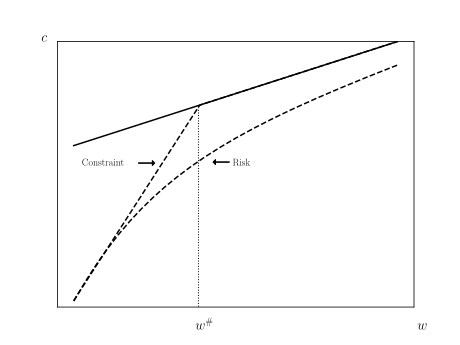
\includegraphics[width=.95\textwidth]{\FigDir/CounterclockwiseConcavifications}}
	\caption{Examples of Counterclockwise Concavifications}
	{\footnotesize \begin{singlespace} {\emph{Notes:} The solid line shows the linear consumption function in the case with no constraints and no risks. The two dashed line show the consumption function when we introduce a constraint and a risk, respectively. The introduction of a constraint is a counterclockwise concavification of the solid consumption function around $w^{\#}$, while the introduction of a risk is a counterclockwise concavification around $\infty$.}  \end{singlespace}}
	\label{fig:counterclockwise}
\end{figure}



%%%Further, the concept is strict in the sense that these properties hold with strict inequality for at least one $\wAlt < w^{\#}$. %(This is a generalization of the
%%%original situation considered in theorem~\ref{thm:CCToPrud} in the
%%%sense that the original proof can be thought of as a specialization of
%%%this setup in the case where $w^{\#}$ approaches infinity and
%%%where the initial consumption function is restricted to linearity).
%%%We will also need to define a sense in which $\hat{c}_{t}(w_{t})$ is a
%%%global counterclockwise concavification of $c_{t}(w_{t})$.
%%%\begin{defn}\label{defn:multcc} (Global Counterclockwise Concavification). \\
%%%	Function $\hat{c}_{t}(w_{t})$ is a global counterclockwise
%%%	concavification of $c_{t}(w_{t})$ if $\hat{c}_{t}(w_{t})$ can be
%%%	constructed from $c_{t}(w_{t})$ by a sequence of counterclockwise concavifications around a set of points $\vec{\wAlt}$.
%%%\end{defn}




\subsection{Consumption Concavity and Prudence}
The section above established all the tools necessary to show the relationship between consumption concavity and prudence.
%%%Our first result is that locally strictly greater consumption concavity implies that the value function also exhibits strictly greater absolute prudence at that point.
%%%\begin{theorem}\label{the:ccandprud}(Local Consumption Concavity and Prudence). \\
%%%	If $\hat{V}$ exhibits strictly greater CC than $V$ at point
%%%	$w$, then absolute prudence of $\hat{V}(w)$ is greater
%%%	than absolute prudence of $V(w)$.
%%%\end{theorem}
%%%
%%%\begin{proof} \citet{kimball:smallandlarge} shows that greater prudence can be defined as $\hat{V}'(w)$ being a convex function of
%%%	$V'(w).$ But since $V'(w) = u'(c(w))$
%%%	and $\hat{V}'(w) = u'(\hat{c}(w))$ for the same
%%%	monotonically downward sloping $u'$, greater CC of $\hat{V}$ than
%%%	$V$ at $w$ implies that $\hat{V}'(w)$ is a convex function of $V(w)$.
%%%\end{proof}
%%%Note that Theorem \ref{the:ccandprud} holds only locally. To say something about global properties, we need our concept of counterclockwise concavification. For the next two results,
Our method in this section is to compare prudence in a \textit{baseline} case where the consumption function is $c(w)$ to prudence in a \textit{modified} situation in which the consumption function $\hat{c}(w)$ is a counterclockwise concavification of the baseline consumption function.
%%%We proceed by analyzing each of the three cases: CRRA, CARA, and quadratic utility.

%%%\subsubsection{The CRRA Case}\label{subsubsec:CRRACase}
%%%\ifthenelse{\boolean{Outline}}{ %\ref{subsec:DefHARACCPrud}
%%%\immediate{\write18{echo "...."  CRRACase >> ./Index.txt}}}{}
%%%
%%%
%%%Our first baseline $c(w)$ will be the linear consumption
%%%function that arises under CRRA utility in the absence of labor income
%%%risk or constraints.\footnote{The analysis below goes through even if
%%%  there is rate-of-return risk in the problem, so long as the
%%%  rate-of-return risk is not modified when the labor income risk is
%%%  added.} Below  we show that imposing a
%%%constraint concavifies the consumption function.  Similarly, \citet{carroll&kimball:concavity} show that the addition of
%%%labor income risk renders the risk-modified consumption rule concave.
%%%In either case it is possible to show that as wealth approaches
%%%infinity the consumption rule in the modified situation
%%%$\hat{c}(w_t)$ approaches the consumption rule in the baseline
%%%situation.  When the experiment is the imposition of a liquidity
%%%constraint, $\hat{c}(w)$ approaches $c(w)$
%%%because as wealth approaches infinity the constraint becomes
%%%irrelevant because the probability that it will ever bind becomes
%%%zero.  When the treatment is the addition of labor income risk,
%%%$\hat{c}(w)$ approaches $c(w)$ because as wealth
%%%approaches infinity the portion of future consumption that the
%%%consumer plans on financing out of the uncertain labor income stream
%%%becomes vanishingly small.\footnote{Since in the CRRA case the
%%%  proportionate effect of risk on consumption depends on the {\it
%%%    square} of the standard deviation of the risk relative to wealth,
%%%  as this ratio gets small as wealth approaches infinity, the absolute
%%%  size of the effect of the risk in reducing consumption approaches
%%%  zero.} Formally, we can capture both the liquidity constraint and
%%%the precautionary saving cases with the assertion that
%%%\[
%%%\lim_{w\rightarrow \infty} \hat{c}(w)-c(w) = 0.
%%%\]

\begin{theorem}\label{thm:CCToPrud}  (Counterclockwise Concavification and Prudence). \\
	Consider an agent who has a utility function %of the HARA class \eqref{eq:HARA}
	with $u' > 0$, $u'' < 0$, $u''' \geq 0$, and non-increasing absolute prudence $-u'''/u''$. If $c(w)$ is concave and $\hat{c}(w)$ is a counterclockwise concavification of $c(w)$, then the value function associated with $\hat{c}(w)$ exhibits greater prudence than the value function associated with $c(w)$ for all $w$.
\end{theorem}
\noindent See Appendix \ref{app:CCToPrud} for the proof.
There are two channels through which a counterclockwise concavification heightens prudence. First, if the absolute prudence of the utility function is non-increasing, then the reduction in consumption and increase in MPC from the counterclockwise concavification make households more prudent. Second, the increase in consumption concavity from the counterclockwise concavification itself also heightens prudence. The channels operate separately, implying that a counterclockwise concavification heightens prudence \textit{even if absolute prudence is zero} as in the quadratic case.

Theorem \ref{thm:CCToPrud} only provides conditions for when the value function exhibits greater prudence, but not strictly greater prudence. In particular, the value function associated with $\hat{c}(w)$ will in some cases exhibit equal prudence for many values of $w$ and strictly greater prudence only for some values of $w$. In Corollary \ref{cor:ccandstrictprud}, we provide conditions for when the value function exhibits strictly greater prudence.

\begin{corollary} \label{cor:ccandstrictprud}(Counterclockwise Concavification and Strictly Greater Prudence).\\
	Consider an agent who has a utility function with $u' > 0$, $u'' < 0$, $u''' \geq 0$, and non-increasing absolute prudence $-u'''/u''$. If $c(w)$ is concave and $\hat{c}(w)$ is a counterclockwise concavification of $c(w)$, then the value function associated with $\hat{c}(w)$ exhibits strictly greater prudence than the value function associated with $c(w)$ at $w$ if the utility function satisfies $u''' > 0$ and $w < w^{\#}$ (the point of counterclockwise concavification) or the utility function is quadratic ($u''' = 0$) and $\frac{\hat{c}'(w)}{c'(w)}$ strictly declines at $w$.
\end{corollary}
\noindent See Appendix \ref{app:ccandstrictprud} for the proof. For prudent households ($u''' > 0$), the value function exhibits strictly greater prudence for all levels of wealth where the counterclockwise concavification affects consumption. This is a result of the fact that a reduction in consumption and higher marginal propensity to consume heighten prudence if the utility function has a positive third derivative and prudence is non-increasing. If the utility function instead is quadratic, the third derivative is zero and the absolute prudence of the utility function does not depend on the level of consumption or the marginal propensity to consume. In this case, the counterclockwise concavification only affects prudence at the kink points in the consumption function, i.e. where $\frac{\hat{c}'(w)}{c'(w)}$ strictly declines at $w$.



%%%\begin{theorem}
%%%	\noindent \textbf{Case I (CRRA utility):}
%%%	\begin{enumerate}
%%%	\item If optimal consumption in the baseline situation is described by a neoclassical consumption function $c_t(w_t)$ that is linear, while optimal behavior in the modified situation (indicated by a hat) is described by a concave neoclassical consumption function $\hat{c}_t(w_{t})$ and if $\displaystyle \lim_{w_{t} \rightarrow + \infty} \hat{c}_t(w_{t}) - c_t(w_{t}) = 0,$ then at any given level of wealth $w_{t}$ the value function in the modified situation exhibits greater absolute prudence than in the baseline situation.  Prudence at $w_t$ in the modified situation is strictly greater if and only if the modified consumption function is strictly concave at some wealth level at or above $w_{t}$.
%%%	\item If the optimal neoclassical consumption function in the baseline
%%%	situation $c_{t}(w_{t})$ is concave and $\hat{c}_{t}(w_{t})$ is a
%%%	counterclockwise concavification of $c_{t}(w_{t})$ around
%%%	$w^{\#}$, then the value function associated with
%%%	$\hat{c}_{t}(w_{t})$ exhibits greater prudence than the value
%%%	function associated with $c_{t}(w_{t})$.  Prudence at $w_{t}$ is
%%%	strictly greater in the modified situation than in the baseline
%%%	situation all levels of wealth $w_{t}$ below $w^{\#}$.
%%%	\end{enumerate}
%%%\textbf{Case II (CARA utility):} If the consumption function in the modified situation $\hat{c}_{t}(w_{t})$ is a counterclockwise concavification of the consumption function in the baseline situation and $\displaystyle \lim_{w_{t} \rightarrow + \infty}\hat{c}_t(w_{t}) - c_t(w_{t}) \leq 0$, then the value function in the modified situation has greater absolute prudence at $w_{t}$ than does the value function for baseline situation.  The inequality of prudence is strict if the modified consumption function is strictly concave at or above $w_{t}$.
%%%
%%%	\bigskip
%%%	\noindent \textbf{Case III (Quadratic utility):} Consider an agent who has a quadratic utility function in two
%%%	different situations. If the baseline situation has a consumption function that is concave over some range $w_{t}<\wAlt$ and the consumption function in the	modified situation is a counterclockwise concavification of
%%%	$c_{t}(w_{t}),$ prudence of $\hat{V}_{t}(w_{t})$ will be strictly greater than prudence of $V_{t}(w_{t})$ at points where
%%%	$\hat{c}_{t}'(w_{t})/c_{t}'(w_{t})$ strictly declines.
%%%\end{theorem}
%%%
%%%

%%%\begin{theorem} \label{thm:CCToPrud}
%%%  Consider an agent who has a utility function with $u'(c)> 0$,
%%%  $u''(c)<0$, $u'''(c) > 0$ and non-increasing absolute prudence
%%%  $-u'''(c)/u''(c)$ in two different situations.  If optimal
%%%  consumption in the baseline situation is described by a neoclassical
%%%  consumption function $c_t(w_t)$ that is linear, while optimal
%%%  behavior in the modified situation (indicated by a hat) is described
%%%  by a concave neoclassical consumption function $\hat{c}_t(w_{t})$
%%%  and if $\displaystyle \lim_{w_{t} \rightarrow + \infty}
%%%  \hat{c}_t(w_{t}) - c_t(w_{t}) = 0,$ then at any given level of
%%%  wealth $w_{t}$ the value function in the modified situation exhibits
%%%  greater absolute prudence than in the baseline situation.  Prudence
%%%  at $w_t$ in the modified situation is strictly greater if and only
%%%  if the modified consumption function is strictly concave at some
%%%  wealth level at or above $w_{t}$.
%%%\end{theorem}

%%%\begin{proof} By the envelope theorem, the marginal value of wealth is
%%%always equal to the marginal utility of consumption as long as it is
%%%possible to spend \textit{current} wealth for \textit{current} consumption.
%%%That is,
%%%\begin{eqnarray}
%%%    V'_t(w_t)     & = & u'(c_t(w_t))
%%%\\ \hat V'_t(w_t) & = & u'(\hat{c}_t(w_t)).
%%%\end{eqnarray}
%%%Differentiating each of these equations with respect to
%%%$w_t$,\footnote{Since $\hat{c}(w_t)$ is concave, it has left-hand and
%%%right-hand derivatives at every point, though the left-hand and
%%%right-hand derivatives may not be equal.  Equation
%%%(\ref{eq:hatvpp=uppcp}) should be interpreted accordingly as applying
%%%to left-hand and right-hand derivatives separately.  (Reading
%%%(\ref{eq:hatvpp=uppcp}) in this way implies that $\hat{c}'_t(w_t^-)
%%%\geq \hat{c}'_t(w_t^+)$; therefore $\hat{V}''(w_t^-) \leq \hat{V}''(w_t^+)$).}
%%%\begin{eqnarray}
%%%          V''_t(w_t) & = & u''(c_t(w_t)) c'_t(w_t)  \label{eq:vpp=uppcp}
%%%\\  \hat{V}''_t(w_t) & = & u''(\hat{c}_t(w_t)) \hat{c}'_t(w_t). \label{eq:hatvpp=uppcp}
%%%\end{eqnarray}
%%%
%%%Taking another derivative can run afoul of the possible discontinuity in
%%%$\hat{c}'_t(w_t)$ that we will show below can arise from liquidity constraints, but to establish intuition it is useful to consider
%%%first the case where $\hat{c}''_t(w_t)$ exists; we will then adapt the
%%%proof for the case where $\hat{c}''_t(w_t)$ does not exist.  For the
%%%baseline linear consumption function,
%%%\begin{eqnarray}
%%%V'''_t(w_t) & = & u'''(c_t(w_t)) [c'_t(w_t)]^2 + u''(c_{t}(w_{t}))[c_{t}''(w_{t})]
%%%\\ & = & u'''(c_t(w_t)) [c'_t(w_t)]^2,
%%%\end{eqnarray}
%%%where the second line follows because with a linear consumption
%%%function $c''_t(w_t) = 0$.  Thus,
%%%\[ \mbox{Absolute Prudence} = \frac{-V'''_t(w_t)}{V''_t(w_t)} =
%%%\left(\frac{-u'''(c_t(w_t))}{u''(c_t(w_t))}\right) c'_t(w_t).\]
%%%In the modified situation with a concave consumption function, where
%%%$\hat{c}''_t(w_t)$ exists,
%%%\begin{eqnarray}
%%%    \hat{V}'''_t(w_t) & = & u'''(\hat{c}_t(w_t)) [\hat{c}'_t(w_t)]^2 + u''(\hat{c}_{t}(w_{t}))[\hat{c}_{t}''(w_{t})]
%%%\\   -\frac{\hat{V}'''_t(w_t)}{\hat{V}''_t(w_t)}  & = & - \left(\frac{u'''(\hat{c}_t(w_t)) [\hat{c}'_t(w_t)]^2 + u''(\hat{c}_{t}(w_{t}))[\hat{c}_{t}''(w_{t})] }{u''(\hat{c}_t(w_t)) \hat{c}'_t(w_t)}\right)
%%%\\   -\frac{\hat{V}'''_t(w_t)}{\hat{V}''_t(w_t)}  & = &  \left(\frac{-u'''(\hat{c}_t(w_t))}{u''(\hat{c}_t(w_t))}\right)\hat{c}'_t(w_t) - \frac{\hat{c}''_t(w_t)}{\hat{c}'_t(w_t)}.
%%%\end{eqnarray}
%%%
%%%
%%%\ifthenelse{\boolean{Figures}}{
%%%\begin{figure}
%%% \centerline{\includegraphics[]{Math/CompareCFuncs.eps}}
%%%\ifthenelse{\boolean{FigFileNames}}{\centerline{\tiny CompareCFuncs.eps}}{}
%%% \caption{Consumption Functions in the Baseline and Modified Cases}
%%% \label{fig:CompareCFuncs}
%%%\end{figure}
%%%}
%%%
%%%As can be seen from Figure~\ref{fig:CompareCFuncs},\footnote{This
%%%  figure was generated using simulation programs written for
%%%  Carroll~\cite{carroll:atheorynberwp}; these programs are available
%%%  on Carroll's web page.  The parameterization is as follows.  The
%%%  coefficient of relative risk aversion is $\rho=2$, the time
%%%  preference factor is $\beta=0.95$, the gross interest factor is
%%%  $R=1.04$, the growth factor for permanent income is $G=1.01$.  The
%%%  stochastic process for transitory income for $\hat{c}(w)$ involves a
%%%  small probabilitly (0.005) that income will be zero; if it is not
%%%  zero, then the transitory shock is lognormally distributed with
%%%  standard deviation of 0.2.  Both rules reflect the limit as the
%%%  number of remaining periods of life approaches infinity.} the
%%%assumption that the two consumption functions converge asymptotically,
%%%$\displaystyle \lim_{w_t \rightarrow + \infty} \hat{c}_t(w_t) -
%%%c_t(w_t) = 0, $ together with the linearity of $c_t(w_t)$ and
%%%concavity of $\hat c_t(w_t)$, guarantees that the marginal propensity
%%%to consume is higher and the level of consumption lower in the
%%%modified situation, $\hat c'_t(w_t) \geq c'_t(w_t)$ and
%%%$\hat{c}_t(w_t) \leq c_t(w_t)$.  The inequalities are strict if there
%%%is any strictness to the concavity of $\hat{c}_t(\cdot)$ at any level
%%%of wealth above $w_t$.
%%%
%%%In conjunction with the assumption of non-increasing absolute prudence
%%%of the utility function, $\hat{c}_t(w_t) \leq c_t(w_t)$ implies that
%%%\begin{equation}
%%%\frac{-u'''(\hat{c}_t(w_t))}{u''(\hat{c}_t(w_t))} \geq \frac{-u'''(
%%%c_t(w_t))}{u''(c_t(w_t))}.
%%%\end{equation}
%%%
%%%Therefore, where $\hat{c}''_t(w_t)$ exists,
%%%\begin{eqnarray}
%%%-\frac{\hat{V}'''_t(w_t)}{\hat{V}''_t(w_t)} & = &
%%% \left(\frac{-u'''(\hat{c}_t(w_t))}{u''(\hat{c}_t(w_t))}\right)
%%%\hat{c}'_t(w_t) -
%%%\underbrace{\overbrace{\hat{c}''_t(w_t)}^{\leq 0}/\overbrace{\hat{c}'_t(w_t)}^{>0}}_{\leq 0} \label{eq:vhatprud} \\
%%%& \geq &
%%% \left(\frac{-u'''(c_t(w_t))}{u''(c_t(w_t))}\right) c'_t(w_t) \label{eq:prudence} \\ & = &
%%%-\frac{V'''_t(w_t)}{V''_t(w_t)}.
%%%\end{eqnarray}
%%%That is, concavity of $\hat{c}_{t}(w_{t})$ along with $\lim_{w_{t}
%%%\rightarrow \infty} c_{t}(w_{t})-\hat{c}_{t}(w_{t}) = 0$ implies
%%%that the absolute prudence of $\hat{V}_{t}(w_{t})$ is greater than the
%%%absolute prudence of $V_{t}(w_{t})$.
%%%
%%%Even when the absolute prudence of the utility function is constant,
%%%(\ref{eq:prudence}) is strict whenever either (1) $\hat{c}_t(\cdot)$
%%%is strictly concave at some level of wealth above $w_t$
%%%(because, with weak concavity everywhere, strict concavity anywhere
%%%above $w_{t}$ implies that $\hat{c}'_t(w_t) > c'_t(w_t)$); or (2)
%%%$\hat{c}_t(\cdot)$ is strictly concave exactly \textit{at} $w_t$ (because
%%%strict concavity at $w_{t}$ implies that $-\frac{\hat
%%%c''_t(w_t)}{\hat{c}'_t(w_t)}>0$).  Conversely, if
%%%$\hat{c}_t(\cdot)$ is linear at $w_t$ and all higher levels of wealth,
%%%(\ref{eq:prudence}) clearly holds with equality.  We can summarize by
%%%saying that the inequality (\ref{eq:prudence}) which expresses the
%%%result of the theorem is \textit{strict} if and only if
%%%$\hat{c}_t(\cdot)$ is strictly concave at or above $w_t$.
%%%
%%%What if $\hat{c}''_t(w_t)$ and $\hat{V}'''_t(w_t)$ do not exist?
%%%Informally, if nonexistence is caused by a constraint binding at
%%%$w_{t}$, the effect will be a discrete decline in the marginal propensity
%%%to consume at $w_{t}$, which can be thought of as $\hat{c}_{t}^{\prime\prime}(w_{t}) = -\infty$,
%%%implying positive infinite prudence at that point (see \eqref{eq:vhatprud}).
%%%Formally, if $\hat{c}_{t}^{\prime\prime}(w_{t})$ does not exist
%%%greater prudence of $\hat{V}_{t}$ than $V_{t}$ is defined as
%%%$\frac{\hat {V}''_t(w_t)}{V''_t(w_t)}$ being a decreasing function of
%%%$w_t$.  By (\ref{eq:vpp=uppcp}) and (\ref{eq:hatvpp=uppcp}),
%%%\begin{equation}
%%%\frac{\hat{V}''_t(w_t)}{V''_t(w_t)} \equiv
%%%\left(\frac{u''(\hat c_t(w_t))}{u''(c_t(w_t))} \right)
%%%\left(\frac{\hat{c}'_t(w_t)}{c'_t(w_t)}\right).  \label{eq:vppratios}
%%%\end{equation}
%%%
%%%The second factor, $\frac{\hat{c}'_t(w_t)}{c'_t(w_t)}$, is globally
%%%decreasing (see Figure~\ref{fig:CompareCFuncs}; it declines
%%%monotonically toward 1).  At any specific value of $w_t$ where
%%%$\hat{c}_t''(w_t)$ does not exist because the left and right hand
%%%values of $\hat{c}'_t$ are different, we say that $\hat{c}'_{t}$
%%%is decreasing if
%%%\begin{eqnarray}
%%%  \lim_{w^{-} \rightarrow w} \hat{c}'_t(w_t) & > & \lim_{w^{+} \rightarrow w} \hat{c}'_t(w_t).
%%%\end{eqnarray}
%%%
%%%As for the first factor, note that nonexistence of
%%%$\hat{V}'''_{t}(w_{t})$ and/or $\hat{c}_{t}''(w_{t})$ do not
%%%spring from nonexistence of either $u'''(c)$ or $\lim_{w \uparrow
%%%  w_t} \hat{c}_{t}'(w)$ (for our purposes, when the
%%%left and right derivatives of $\hat{c}_t(w_t)$ differ at a point, the
%%%relevant derivative is the one coming from the left; rather than carry
%%%around the cumbersome limit notation, read the following derivation as
%%%applying to the left derivative).  To discover whether $\frac{\hat
%%%  {V}''_t(w_t)}{V''_t(w_t)}$ is decreasing we can simply
%%%differentiate:
%%%\begin{eqnarray}
%%%     \frac{d}{d w_{t}}\left( \frac{u''(\hat{c}_t(w_{t}))}{ u''(c_t(w_{t}))}\right) &=& \frac{u'''(\hat{c}_{t}(w_{t}))\hat{c}_{t}'(w_{t})u''(c_{t}(w_{t}))-u''(\hat{c}_{t}(w_{t}))u'''(c_{t}(w_{t}))c'_{t}(w_{t})}{[u''(c_{t}(w_{t}))]^{2}}. \qquad \qquad
%%%\end{eqnarray}
%%%
%%%Since the denominator is always positive, this will be negative if the
%%%numerator is negative, i.e.  if
%%%\begin{eqnarray}
%%%    u'''(\hat{c}_{t}(w_{t}))u''(c_{t}(w_{t}))\hat{c}_{t}'(w_{t}) & \leq & u''(\hat{c}_{t}(w_{t}))u'''(c_{t}(w_{t}))c'_{t}(w_{t})
%%%\\  \left(\frac{u'''(\hat{c}_{t}(w_{t}))}{u''(\hat{c}_{t}(w_{t}))}\right)\hat{c}_{t}'(w_{t}) & \leq & \left(\frac{u'''(c_{t}(w_{t}))}{u''(c_{t}(w_{t}))}\right)c'_{t}(w_{t})
%%%\\  \underbrace{\left(\frac{-u'''(\hat{c}_{t}(w_{t}))}{u''(\hat{c}_{t}(w_{t}))}\right)}_{\mbox{\tiny Absolute prudence at $\hat{c}_{t}(w_{t})$}}\hat{c}_{t}'(w_{t}) & \geq & \underbrace{\left(\frac{-u'''(c_{t}(w_{t}))}{u''(c_{t}(w_{t}))}\right)}_{\mbox{\tiny Absolute prudence at $c_{t}(w_{t})$}} c'_{t}(w_{t}) \label{eq:prudcond} .
%%%\end{eqnarray}
%%%
%%%Recall that $\hat{c}_{t}(w_{t}) \leq c_{t}(w_{t})$ (see figure
%%%\ref{fig:CompareCFuncs}), so the assumption of non-increasing
%%%absolute prudence tells us that the absolute prudence term on the LHS
%%%of \eqref{eq:prudcond} is greater than that on the RHS. But by the
%%%assumption of concavity of $\hat{c}_{t}(w_{t})$ we also know that
%%%$\hat{c}'_{t}(w_{t}) \geq c'_{t}(w_{t})$.  Hence both terms on
%%%the LHS are greater than or equal to the corresponding terms on the
%%%RHS.  The inequality is strict at any point for which
%%%$\hat{c}_t'(w_t) > c_t'(w_t)$.
%%%
%%%Note finally that condition \eqref{eq:prudcond} is equivalent to
%%%our definition of property greater CC for consumption functions for
%%%which $c'(w_{t})$ and $\hat{c}'(w_{t})$ exist in the sense of
%%%left and right derivatives.
%%%
%%%Thus, combining all of the factors involved in comparing the prudence
%%%of $\hat{V}_{t}(w_{t})$ to the prudence of $V_{t}(w_{t})$, we have
%%%shown that the value function in the modified situation will exhibit
%%%strictly greater prudence at any given $w_{t}$ than the value function
%%%in the baseline situation if and only if $\hat{c}_t(w_{t})$ is
%%%strictly concave at $w_t$ or at some level of wealth above $w_t$.
%%%\end{proof}

%%%\subsubsection{Counterclockwise Concavification Causes a Strict Increase in Prudence} \label{subsubsec:MoreCCToMorePrud}

%%%\ifthenelse{\boolean{Outline}}{ %\ref{subsec:DefHARACCPrud}
%%%\immediate{\write18{echo "...."  MoreCCToMorePrud >> ./Index.txt}}}{}

%%%We assumed above that the baseline consumption function was linear.
%%%It will be useful for later purposes to have a slightly more general
%%%analysis.  The idea is to think of the consumption function in the
%%%modified situation as being a twisted version of the consumption
%%%function in the baseline situation, where the kind of twisting allowed
%%%is a progressively larger increase in the MPC as the level of wealth
%%%gets lower.  We call this a `counterclockwise' concavification, to
%%%capture the sense that at any specific level of wealth, we can think
%%%of the increase in the MPC at lower levels of wealth as being a
%%%counterclockwise rotation of the lower portion of the consumption
%%%function around that level of wealth.
%%%
%%%\begin{defn} Function $\hat{c}_{t}(w_{t})$ is a counterclockwise concavification of
%%%$c_{t}(w_{t})$ around $w^{\#}$ if the following conditions hold:
%%%\begin{enumerate}
%%%\item $\hat{c}_{t}(\wAlt) = c_{t}(\wAlt)$ for $\wAlt \geq w^{\#}$
%%%%\item $\lim_{\wAlt \downarrow w^{\#}}  \left(\frac{\hat{c}_{t}'(\wAlt)}{c_{t}'(\wAlt)}\right) = 1$
%%%\item $\lim_{\wAlt \uparrow w_{t}} \left(\frac{\hat{c}_{t}'(\wAlt)}{c_{t}'(\wAlt)}\right)$ is weakly decreasing in $w_{t}$ everywhere below $w^{\#}$
%%%\item $\lim_{\wAlt \uparrow w^{\#}} \left(\frac{\hat{c}_{t}'(\wAlt)}{c_{t}'(\wAlt)}\right)  \geq 1$
%%%\item If $\lim_{\wAlt \uparrow w^{\#}} \left(\frac{\hat{c}_{t}'(\wAlt)}{c_{t}'(\wAlt)}\right)  = 1$, then $\lim_{\wAlt \uparrow w^{\#}} \left(\frac{\hat{c}_{t}''(\wAlt)}{c_{t}''(\wAlt)}\right) > 1$
%%%\end{enumerate}
%%%\end{defn}
%%%where the limits using $\wAlt$ are necessary to allow for the
%%%possibility of discrete drops in the MPC at potential `kink points' in
%%%the two consumption functions.  (This is a generalization of the
%%%original situation considered in theorem~\ref{thm:CCToPrud} in the
%%%sense that the original proof can be thought of as a specialization of
%%%this setup in the case where $w^{\#}$ approaches infinity and
%%%where the initial consumption function is restricted to linearity).

%%%Given definition \ref{defn:cconcavification}, we have
%%%\begin{theorem}\label{thm:MoreCCToMorePrud}
%%%  Consider an agent who satisfies the conditions of
%%%  theorem~\ref{thm:CCToPrud} except that, rather than being linear,
%%%  the optimal neoclassical consumption function in the baseline
%%%  situation $c_{t}(w_{t})$ is concave.  If $\hat{c}_{t}(w_{t})$ is a
%%%  counterclockwise concavification of $c_{t}(w_{t})$ around
%%%  $w^{\#}$ then the value function associated with
%%%  $\hat{c}_{t}(w_{t})$ exhibits greater prudence than the value
%%%  function associated with $c_{t}(w_{t})$.  Prudence at $w_{t}$ is
%%%  strictly greater in the modified situation than in the baseline
%%%  situation all levels of wealth $w_{t}$ below $w^{\#}$.
%%%\end{theorem}

%%%\begin{proof} The proof is identical to the proof of
%%%theorem~\ref{thm:CCToPrud}, except where that proof demonstrates that
%%%$ \left(\frac{\hat{c}_{t}'(w_{t})}{c_{t}'(w_{t})}\right)$ is
%%%weakly decreasing for the setup described in the theorem; that
%%%requirement is now assumed directly.
%%%\end{proof}






%%%\subsubsection{The Exponential Case} \label{subsubsec:ExpCase}
%%%\ifthenelse{\boolean{Outline}}{ %\ref{subsec:DefHARACCPrud}
%%%\immediate{\write18{echo "...."  ExpCase >> ./Index.txt}}}{}


%%%The assumption $\displaystyle \lim_{w_{t} \rightarrow \infty}
%%%\hat{c}_{t}(w_{t} )-c_{t}(w_{t} ) = 0$ will be true if consumers have
%%%CRRA utility and if the difference between the baseline and the
%%%modified situations is the addition of either labor income risk or a
%%%liquidity constraint.  However, if the consumer's utility function is
%%%of the CARA form, a labor income risk simply shifts the entire
%%%consumption function down by an equal amount at all levels of $w_{t}$,
%%%and so the level of consumption in the modified case does not approach
%%%the level in the baseline case as wealth approaches infinity.  We
%%%therefore need a modified version of the theorem to apply in this
%%%case.
%%%
%%%\begin{corollary}\label{cor:expcase}
%%%  Consider an agent who has a utility function with $u'(c)> 0$,
%%%  $u''(c)<0$, $u'''(c) > 0$ and non-increasing absolute prudence
%%%  $-u'''(c)/u''(c)$ in two different situations.
%%%% MorePrud: The following is the new text from the version with concave baseline
%%%If the consumption function in
%%%    the modified situation $\hat{c}_{t}(w_{t})$ is a counterclockwise
%%%    concavification of the consumption function in the baseline
%%%    situation
%%%\begin{Private}\begin{comment} % MorePrud: The following is the old text from the version with a linear baseline
%%%If the baseline situation has a neoclassical consumption function $c_t(w_{t})$ that is linear, while the modified situation (indicated by a hat) has a concave neoclassical consumption function $\hat{c}_t(w_{t})$ and $\displaystyle \lim_{w_{t} \rightarrow + \infty} \hat{c}'_t(w_{t})/c'_t(w_{t}) =   1$
%%%\end{comment}\end{Private}
%%%and $\displaystyle \lim_{w_{t} \rightarrow + \infty}
%%%  \hat{c}_t(w_{t}) - c_t(w_{t}) \leq 0$, then the value function in
%%%  the modified situation has greater absolute prudence at $w_{t}$ than
%%%  does the value function for baseline situation.  The inequality of
%%%  prudence is strict if the modified consumption function is strictly
%%%  concave at or above $w_{t}$.
%%%\end{corollary}

%%%The proof of the corollary follows the proof of the main theorem,
%%%except where $\lim_{w_{t} \rightarrow +\infty}
%%%\hat{c}_{t}(w_{t})-c_{t}(w_{t}) = 0$ and concavity of
%%%$\hat{c}_{t}(w_{t})$ were used to demonstrate that
%%%$\hat{c}_{t}'(w_{t}) \geq c_{t}'(w_{t})$ and that
%%%$\hat{c}_{t}(w_{t}) \leq c_{t}(w_{t})$; here we assume
%%%both propositions.
%%%\begin{Private}\begin{comment} % MorePrud: The following is the old text from the version with a linear baseline
%%%the second, and the first follows from concavity of
%%%  $\hat{c}_{t}(w_{t})$, linearity of $c_{t}(w_{t})$, the assumption
%%%  that $\lim_{w_{t} \rightarrow \infty}
%%%  \hat{c}'(w_{t})/c'(w_{t})=1$, and the fact that $\lim_{w_t
%%%    \rightarrow \infty} \hat{c}_{t}(w_{t}) - c_{t}(w_{t}) \leq 0.$
%%%\end{comment}\end{Private}

%%%\subsubsection{The Quadratic Case} \label{subsubsec:QuadCase}
%%%\ifthenelse{\boolean{Outline}}{ %\ref{subsec:DefHARACCPrud}
%%%\immediate{\write18{echo "...."  QuadCase >> ./Index.txt}}}{}
%%%

%%%The quadratic case requires a somewhat different approach.  First, the
%%%limit $w_{t} \rightarrow \infty$ is not as meaningful, since it goes
%%%beyond the bliss point.  Second, since $u'''(\cdot)=0$, strict
%%%inequality between the prudence of $\hat{V}$ and the prudence of $V$
%%%will hold only \textit{at} those points where $\hat{c}_t(\cdot)$ is
%%%strictly concave.
%%%
%%%To gain intuition for the quadratic problem, consider the Euler
%%%equation in the second-to-last period of a lifetime that ends at $T$,
%%%under the assumption that there is no chance that wealth in period $T$
%%%will be greater than the bliss-point level of consumption:\footnote{If
%%%there is a chance that $w_{T}$ could exceed the bliss point, then the
%%%kink point in the period-$T$ consumption rule can impart concavity to
%%%the period-$T-1$ consumption rule.}
%%%\begin{eqnarray}
%%%        u'(c_{T-1}) & = & \Ex_{T-1}\left[\tilde{\beta}_{T}\tilde{R}_{T}u'(\tilde{R}_{T}(w_{T-1}-c_{T-1})+\tilde{y}_{T})\right]  \\
%%%        \alpha (\kappa-c_{T-1}) & = & \Ex_{T-1}\left\{\tilde{\beta}_{T}\tilde{R}_{T}\alpha\left(\kappa-\left[\tilde{R}_{T}(w_{T-1}-c_{T-1})+\tilde{y}_{T}\right]\right)\right\}  \\
%%%        c_{T-1} & = & \frac{\Ex_{T-1}[\tilde{\beta}_{T}\tilde{R}_{T}^{2}w_{T-1}]+\Ex_{T-1}[\tilde{\beta}_{T}\tilde{R}_{T}\tilde{y}_{T}]+\kappa(1-\Ex_{T-1}[\tilde{\beta}_{T}\tilde{R}_{T}])}{1+\Ex_{T-1}[\tilde{\beta}_{T}\tilde{R}_{T}^{2}]}. \label{eq:quadmpc}
%%%\end{eqnarray}
%%%
%%%This equation illustrates the well-known fact that in the quadratic
%%%case in the absence of liquidity constraints and rate-of-return risk,
%%%the solution exhibits certainty equivalence with respect to risks to
%%%labor income $y_{T}$.\footnote{An interesting subtlety is that even though the
%%%solution is linear in wealth, it does \textit{not} exhibit certainty
%%%equivalence with respect to rate-of-return risk, since the level of
%%%consumption is related to the expectation of the \textit{square} of the
%%%gross return, in a way that implies that an increase in rate-of-return
%%%risk increases the marginal propensity to consume.  Note also that
%%%interactions between rate-of-return risk and income risk can cause the
%%%consumption function to shift up or down by a potentially large
%%%amount.}
%%%
%%%Recall now from equation \eqref{eq:vppratios} that greater prudence of
%%%$\hat{V}_{t}(w_{t})$ than $V_{t}(w_{t})$ occurs if
%%%\begin{eqnarray}
%%%    \frac{\hat{V}''_t(w_t)}{V''_t(w_t)} & \equiv & \frac{u''(\hat c_t(w_t))}{u''(c_t(w_t))} \frac{\hat{c}'_t(w_t)}{c'_t(w_t)}
%%%\\  & = & \frac{\hat{c}'_t(w_t)}{c'_t(w_t)} \label{eq:cprimeratios}
%%%\end{eqnarray}
%%%is a decreasing function of $w_{t}$ (the second line follows because
%%%for quadratic utility $u''(c)$ is a constant).
%%%
%%%Thus, prudence of the value function can be increased in the quadratic
%%%case only by something that causes the MPC
%%%to decrease as wealth rises.  We will show below that in the
%%%quadratic case $\hat{c}'_{t}(w_{t})$ experiences a discrete decline
%%%at values of $w_t$ where a future liquidity constraint potentially
%%%begins to impinge on current consumption.  \begin{Private}\begin{comment}Note, however, that an increase in
%%%  rate-of-return risk, while it increases the level of the MPC
%%%  compared to the baseline case, does \textit{not} induce a {\it
%%%    declining} MPC in wealth: The MPC is higher everywhere, but
%%%  constant.  Thus, rate-of-return risk does not induce an increase in
%%%  prudence in the quadratic case because $u'''(c)=0$ for quadratic
%%%  utility functions (cf.  equation \eqref{eq:prudcond}).\end{comment}\end{Private}
%%%
%%%\begin{corollary}\label{cor:quadcase}
%%%  Consider an agent who has a quadratic utility function in two
%%%  different situations.
%%%% MorePrud: New text
%%%If the
%%%    baseline situation has a consumption function that is concave over
%%%    some range $w_{t}<\wAlt$ and the consumption function in the
%%%    modified situation is a counterclockwise concavification of
%%%    $c_{t}(w_{t}),$
%%%% MorePrud: Original text
%%%\begin{Private}\begin{comment}If the baseline situation has a consumption
%%%    function $c_t(w_{t})$ that is linear over some range
%%%    $w_{t}<\wAlt$, while the modified situation has consumption
%%%    function $\hat{c}_{t}(w_{t})$ that exhibits a declining marginal
%%%    propensity to consume for $w_{t}<\wAlt$,
%%%then prudence of
%%%\end{comment}\end{Private}
%%%  prudence of $\hat{V}_{t}(w_{t})$ will be strictly greater than prudence of
%%%  $V_{t}(w_{t})$ at points where
%%%  $\hat{c}_{t}'(w_{t})/c_{t}'(w_{t})$ strictly declines.
%%%\end{corollary}
%%%The proof is simply to note that equation $\eqref{eq:cprimeratios}$
%%%holds only at points where $\hat{c}'_{t}(w_{t})/c_{t}'(w_{t})$
%%%declines with $w_{t}$.

\end{verbatimwrite}\ifVerbatimWrite{\input{Sections/PrudAndCC}}{} %%% Private

\section{Recursive Propagation of Consumption Concavity}\label{sec:Aggregation} 

\begin{verbatimwrite}{Sections/Recursive} %%% Private
  
In section \ref{sec:PrudAndCC}, we provide conditions for when consumption concavity heightens prudence by comparing value functions and consumption functions at a specific point in time. In this section, we provide conditions guaranteeing that if the consumption function is concave in period $t+1$, it will be concave in period $t$ and earlier, whatever the source of that concavity may be.

\begin{theorem}\label{thm:recursive}(Recursive Propagation of Consumption Concavity). \\
	Consider an agent with a HARA utility function satisfying $u' > 0$, $u'' < 0$, $u''' \geq 0$ and non-increasing absolute prudence $-u'''/u''$. Assume that no liquidity constraint applies at the end of period $t$ and that the agent faces income risk $y_{t+1} \in [\underline{y},\bar{y}]$. If $V_{t+1}(w_{t+1})$ exhibits property consumption concavity for all $w_{t+1} \in [Rs_t + \underline{y}, Rs_t + \bar{y}]$, then $V_t(w_t)$ exhibits property consumption concavity at the level of wealth $w_t$ such that optimal consumption yields $s_t = w_t - c_t(w_t)$.

	\medskip
	If also $V_{t+1}(w_{t+1})$ exhibits property strict consumption concavity for at least one $w_{t+1} \in [Rs_t + \underline{y}, Rs_t + \bar{y}]$, then $V_t(w_t)$ exhibits property strict consumption concavity at the level of wealth $w_t$ where optimal consumption yields $s_t = w_t - c_t(w_t)$.
\end{theorem}
See Appendix \ref{app:recursive} for the proof. Theorem \ref{thm:recursive} presents conditions to ensure that the consumption function is concave today if the consumption function is concave in the future. The basic insight is that as long as the future consumption function is concave for all realization of $y_{t+1}$, then it is also concave today. Additionally, if the
the future consumption function is strictly concave for at least one realization of ${y}_{t+1}$, then the consumption function is strictly concave also today. %By combining the results in this section and the previous, we know that if the consumption function is strictly concave at some future time period and the conditions of Theorem \ref{thm:recursive} are satisfied, then the value function exhibits heightened prudence also today.


\end{verbatimwrite}\ifVerbatimWrite{\input{Sections/Recursive}}{} %%% Private

\section{Liquidity Constraints and Consumption Concavity}\label{sec:Precaution} 
\begin{verbatimwrite}{Sections/LCandCC} %%% Private

We now move on to the sources of consumption concavity. In our setting, there are two sources of consumption concavity: risk and constraints. The properties of consumption under risk have already been derived in \citet{carroll&kimball:concavity}. We therefore restrict our attention to showing how liquidity constraints make the consumption function concave. Once the relationship between liquidity constraints and consumption concavity is established, we use the results on consumption concavity and prudence to show under which conditions liquidity constraints increase prudence.
%But before we can start showing the effects of liquidity constraints on consumption, we have to establish some notation.

\subsection{Notation}
Throughout this paper, we are working with a finite horizon household with an horizon going from $0$ to $T$. A liquidity constraint is a constraint on wealth that binds at a specific time $t \in (0, T]$. We first define an ordered set to keep track of the liquidity constraints.
\begin{defn} (The Set of Liquidity Constraints). \\
	We define $\mathcal{T}$ as an ordered set of dates at which a relevant constraint exists. We define $\mathcal{T}[1]$ as the last period in which a constraint exists, and $\mathcal{T}[2]$ is the date of the last period before $\mathcal{T}[1]$ in which a constraint exists, and so on.
\end{defn}
For any $t \in [0, T)$, we define $c_{t,n}$ as the optimal consumption function in period $t$ assuming that the first $n$ constraints in $\mathcal{T}$ have been imposed. For example, $c_{t,0}(w)$ is the consumption function in period $t$ when no constraint (aside from the intertemporal budget constraint) has been imposed, $c_{t,1}(w)$ is the consumption function in period $t$ after the chronologically last constraint has been imposed, and so on. We define $\Omega_{t,n}, V_{t,n}$, and other functions correspondingly.

To have a distinct terminology for the effects of current-period and future-period constraints, we will restrict the use of the term `binds' to the potential effects of a constraint in the period in which it applies (`the constraint binds if wealth is less than ...') and will use the term `impinges' to describe the effect of a future constraint on current consumption. We can now define the concept of a kink point.
\begin{defn}(Kink Point). \\
	We define a kink point, $\wAlt_{t,n}$ as the level of wealth at which constraint $n$ stops binding (impinging) on time $t$ consumption.
\end{defn}
A kink point corresponds to a transition from a level of wealth where a current constraint binds or a future constraint impinges, to a level of wealth where that constraint no longer binds or impinges.



\subsection{Perfect Foresight Consumption with Liquidity Constraint}\label{subsec:Piecewise}

We first consider an initial situation in which a consumer is solving a perfect foresight optimization problem with a finite horizon that begins in period $t$ and ends in period $T$. The consumer begins with wealth $w_{t}$ and earns constant income ${y}$ in each period. Wealth accumulates according to $w_{t+1} = Rs_{t}+{y}$. We are interested in how this consumer's behavior in period $t$ changes from an initial situation with $n\geq 0$ constraints to a situation in which $n+1$ liquidity constraints has been imposed.

\begin{theorem}\label{thm:pfclc}(Perfect Foresight Consumption with Liquidity Constraints). \\
	Consider an agent who has a utility function with $u'> 0 $ and $u'' < 0$, faces constant income ${y}$, and is `absolutely impatient' (by which we mean $\beta R < 1$). Assume that the agent faces a set $\mathcal{T}$ of $N$ relevant constraints. Then $c_{t,n+1}(w)$ is a counterclockwise concavification of $c_{t,n}(w)$ around $\wAlt_{t,n+1}$ for all $n \leq N-1$
%%%	\begin{enumerate}
%%%		\item $c_{t,n+1}(w) < c_{t,n}(w)$ for $w <\wAlt_{t,n+1}$ and $c_{t,n+1}(w) = c_{t,n}(w)$ for $w \geq \wAlt_{t,n+1}$.
%%%		\item $c_{t,n+1}'(w) > c_{t,n}'(w)$ for $w <\wAlt_{t,n+1}$ and $c_{t,n+1}'(w) = c_{t,n}'(w)$ for $w \geq \wAlt_{t,n+1}$.
%%%		\item $c_{t,n+1}(w)$ is a counterclockwise concavification of $c_{t,n}(w)$ around $\wAlt_{t,n+1}$.
%%%	\end{enumerate}
\end{theorem}

See Appendix \ref{app:pfclc} for the proof. Theorem \ref{thm:pfclc} shows that when we have an ordered set of constraints, $\mathcal{T}$, the introduction of the next constraint in the set represents a counterclockwise concavification of the consumption function. Note that constraint $n+1$ is always at a date prior to the set of the $n$ first constraints. From the proof of Theorem \ref{thm:pfclc}, we also know the shape of the perfect foresight consumption function with liquidity constraints:

\begin{corollary}(Piecewise Linear Consumption Function). \\
	Consider an agent who has a utility function with $u'> 0$ and $u'' < 0$, faces constant income ${y}$, and is absolutely impatient. Assume that the agent faces a set $\mathcal{T}$ of $N$ relevant constraints. When $n \leq N$ constraints have been imposed, $c_{t,n}(w)$ is a piecewise linear increasing concave function with kink points at successively larger values of wealth at which future constraints stop impinging on current consumption.
\end{corollary}

Since the consumption function is piecewise linear, the new consumption function, $c_{t,n+1}(w)$ is not necessarily strictly more concave than $c_{t,n}(w)$ for all $w$. This is where the concept of counterclockwise concavification is useful. Even though $c_{t,n+1}(w)$ is not strictly more concave than $c_{t,n}(w)$ everywhere, it is a counterclockwise concavification and we apply Theorem \ref{thm:CCToPrud} to derive the consequences of imposing one more constraint on prudence.

\begin{theorem}\label{thm:lcip} (Liquidity Constraints Increase Prudence). \\
	Consider an agent in period $t$ who has a utility function with $u' > 0$, $u'' < 0$, $u''' \geq 0$ and non-increasing absolute prudence $-u'''/u''$, faces constant income ${y}$, and is impatient, $\beta R < 1$. Assume that the agent faces a set $\mathcal{T}$ of $N$ relevant constraints. When $n \leq N-1$ constraints have been imposed, the imposition of constraint $n+1$ strictly increases absolute prudence of the agent's value function if $u''' > 0$ and $w_t < \wAlt_{t,n+1}$ or if $u''' = 0$ and $\frac{c'_{t,n+1}}{c'_{t,n}}$ strictly declines at $w$.
%%%	Then the successive imposition of each of the first $\mathcal{R}_{\tau}(w)$ constraints in $\mathcal{T}$ (strictly) increases absolute prudence of the agent's value function in period $\tau$ at wealth $w$. Imposition of any remaining constraints beyond constraint number $\mathcal{R}_{\tau}(w)$ has no effect on the absolute prudence of the value function at $w$ in period $\tau$.
\end{theorem}
\begin{proof}
	By Theorem \ref{thm:pfclc}, the imposition of constraint $n+1$ constitutes a counterclockwise concavification of $c_{t,n}(w)$. By Theorem \ref{thm:CCToPrud} and Corollary \ref{cor:ccandstrictprud}, such a concavification strictly increases absolute prudence of the value function for the cases in Corollary \ref{cor:ccandstrictprud}.
\end{proof}

Theorem \ref{thm:lcip} is the main result in the current section: the introduction of the next liquidity constraint increases absolute prudence of the value function. In the subsequent discussions, we consider cases where we relax the assumptions underlying Theorem \ref{thm:lcip}. We first consider the case where we add an extra constraint to the set of relevant constraints. Next, we consider the cases with time-varying deterministic income, general constraints, and no assumption on time discounting.






\subsection{Increasing the Number of Constraints}
\label{subsec:IncreaseNumConstr}

In the previous section, we analyzed a case where there was a preordained set
of constraints $\mathcal{T}$ which were applied sequentially.  We now examine how behavior will be modified if we add a new date to the set of dates at which the consumer is constrained.

Call the new set of dates $\hat{\mathcal{T}}$ with $N+1$ constraints (one more constraint than before), and call the consumption rules corresponding to the new set of dates
$\hat{c}_{t,1}$ through $\hat{c}_{t,N+1}$. Now call $m$ the
number of constraints in $\mathcal{T}$ at dates strictly
greater than $\hat{\tau}$.  Then note that that $\hat{c}_{\hat{\tau},m} =
c_{\hat{\tau},m}$, because at dates after the date at which the new constraint (number $m+1$) is
imposed, consumption is the same as in the absence of the new constraint.
Now recall that imposition of the constraint at $\hat{\tau}$ causes a counterclockwise concavification of the consumption function around a new kink point, $\wAlt_{\hat{\tau},m+1}$. That is, $\hat{c}_{\hat{\tau},m+1}$ is a counterclockwise concavification of $\hat{c}_{\hat{\tau},m} = c_{\hat{\tau},m}$.

The most interesting observation, however, is that behavior under
constraints $\hat{\mathcal{T}}$ in periods strictly before
$\hat{\tau}$ \textit{cannot} be described as a counterclockwise
concavification of behavior under $\mathcal{T}$.  The reason
is that the values of wealth at which the earlier constraints caused
kink points in the consumption functions before period $\hat{\tau}$ will not generally correspond to kink points once the extra constraint has been added.

\hypertarget{CurrConstrHidesFutKink}{}

\begin{figure}[ht]
{\centering 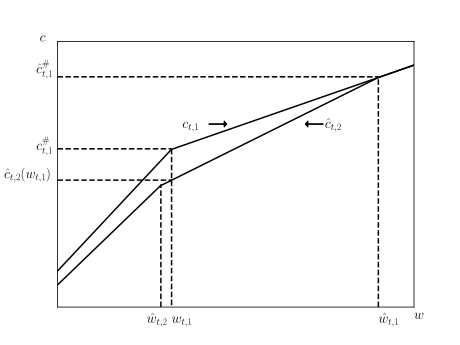
\includegraphics[width=.95\textwidth]{\FigDir/CurrConstrHidesFutKink}}
\caption{How a future constraint can `hide' a current kink}
\footnotesize {\emph{Notes:} $c_{t,1}$ is the original consumption function with one constraint that induces a kink point at $\omega_{t,1}$. $\hat{c}_{t,2}$ is the modified consumption function in where we have introduced one new constraint. The two constraints affect $\hat{c}_{t,2}$ through two kink points: $\hat{\omega}_{t,1}$ and $\hat{\omega}_{t,2}$. Since we introduced the new constraint at a later point in time than the current existing constraint, the future constraint affects the position of the kink induced by the current constraint and the modified consumption function $\hat{c}_{t,2}$ is not a counterclockwise concavification of ${c}_{t,1}$.}
\label{fig:LCtHidesLCtpn}
\end{figure}

We present an example in Figure~\ref{fig:LCtHidesLCtpn}. The original $\mathcal{T}$ contains only a single constraint, at the end of period $t+1$, inducing a kink point at $\wAlt_{t,1}$ in the consumption rule $c_{t,1}$. The expanded set of constraints, $\hat{\mathcal{T}}$, adds one constraint at period $t+2$. $\hat{\mathcal{T}}$ induces two kink points in the updated consumption rule $\hat{c}_{t,2}$, at $\hat{\wAlt}_{t,1}$ and $\hat{\wAlt}_{t,2}$.  It is true that imposition of the new constraint causes consumption to be lower than before at every level of wealth below $\hat{\wAlt}_{t,1}$.  However, this does not imply higher prudence of the value function at every $w <\hat{\wAlt}_{t,1}$.  In particular, note that the original consumption function is strictly concave at $w = \wAlt_{t,1}$, while the new consumption function is linear at $\wAlt_{t,1}$, so prudence can be greater before than after imposition of the new constraint at this particular level of wealth.

The intuition is simple: At levels of initial wealth below $\hat{\wAlt}_{t,1}$, the consumer had been planning to end period $t+2$ with negative wealth. With the new constraint, the old plan of ending up with negative wealth is no longer feasible and the consumer will save more for any given level of current wealth below $\hat{\wAlt}_{t,1}$, including $\wAlt_{t,1}$. But the reason $\wAlt_{t,1}$ was a kink point in the initial situation was that it was the level of wealth where consumption would have been equal to wealth in period $t+1$. Now, because of the extra savings induced by the constraint in $t+2$, the larger savings induced by wealth $\wAlt_{t,1}$ implies that the period $t+1$ constraint will no longer bind for a consumer who begins period $t$ with wealth $\wAlt_{t,1}$. In other words, at wealth $\wAlt_{t,1}$ the extra savings induced by the new constraint `hides' the original constraint and prevents it from being relevant any more at $\wAlt_{t,1}$.

Notice, however, that all constraints that existed in $\mathcal{T}$ will remain relevant at \textit{some} level of wealth under $\hat{\mathcal{T}}$ even after the new constraint is imposed - they just induce kink points at different levels of wealth than before, e.g. the first constraint causes a kink at $\hat{\wAlt}_{t,1}$ rather than at $\wAlt_{t,1}$.

\subsection{A More General Analysis}
\label{subsubsec:MoreGenConstr}

We now want to allow time variation in the level of income,
${y}_{t},$ and in the location of the liquidity constraint
(e.g$.$ a constraint in period $t$ might require the consumer to
end period $t$ with savings $s_{t}$ greater than $\sConst$ where
$\sConst$ is a negative number).  We also drop the restriction that
$\beta R < 1$, allowing the consumer to want to have consumption growth over time.

Under these more general circumstances, a constraint imposed in a
given period can render constraints in either earlier or later periods
irrelevant.  For example, consider a CRRA utility consumer with
$\beta R=1$ who earns income of 1 in each
period, but who is required to arrive at the end of period $T-2$ with
savings of 5.  Then a constraint that requires savings to be greater
than zero at the end of period $T-3$ will have no effect because
%%%withan income of only 1 and a CRRA utility function that requires positive
%%%consumption,
the consumer is required by the constraint in period
$T-2$ to end period $T-3$ with savings greater than 4.

%%%Also, a
%%%constraint that requires the consumer to end period $T-1$ with
%%%positive net worth will also not have any significance for behavior in
%%%periods prior to $T-2$, because any consumer who satisfies the $T-2$
%%%constraint will optimally choose to have positive savings in period
%%%$T-1$ anyway.

Formally, consider now imposing the first constraint, which applies in
period $\tau < T$.  The simplest case, analyzed before, was a
constraint that requires the minimum level of end-of-period wealth
to be $s_{\tau} \geq 0$.  Here we generalize this to $s_{\tau} \geq
\sConst_{\tau,2}$ where in principle we can allow borrowing by choosing
$\sConst$ to be a negative number.  Now for constraint $2$ calculate the kink points for prior periods from
\begin{eqnarray}
  \label{eq:5}
  u'(c_{\tau,2}^{\#}) & = & R\beta u'(c_{\tau+1,1}(R\sConst_{\tau,1}+{y}_{t+1}))
\\ \wAlt_{\tau,2} & = & (V_{\tau,1}')^{-1}(u'(c_{\tau,2}^{\#})).
\end{eqnarray}
In addition, for constraint $2$ recursively calculate
\begin{eqnarray}
\underline{\sConst}_{\tau,2} & = & (\sConst_{\tau+1,2}-{y}_{\tau+1,2}+\underline{c})/R  \label{eq:cgt0}
\end{eqnarray}
where $\underline{c}$ is the lowest value of consumption permitted
by the model (independent of constraints).\footnote{For example, CRRA utility
is well defined only on the positive real numbers, so for a CRRA
utility consumer $\underline{c}=0$.  In other cases, for example with exponential or quadratic
cases, there is nothing to prevent consumption of $-\infty$, so for
those models $\underline{c}=-\infty$, unless there is a desire to
restrict the model to positive values of consumption, in which case
the $c\geq 0$ constraint will be implemented through the use
of \eqref{eq:cgt0}.}

Now assume that the first $n$ constraints in $\mathcal{T}$
have been imposed, and consider imposing constraint number $n+1$,
which we assume applies in period $\tau$.  The first thing to check is
whether constraint number $n+1$ is relevant given the already-imposed
set of constraints.  This is simple: A constraint that requires
$s_{\tau} \geq \sConst_{\tau,n+1}$ will be irrelevant if $\min_{i}
[\underline{\sConst}_{\tau,i}] \leq \sConst_{\tau,n+1}$.  If the
constraint is irrelevant then the analysis proceeds simply by dropping
this constraint and renumbering the constraints in
$\mathcal{T}$ so that the former constraint $n+2$ becomes
constraint $n+1$, $n+3$ becomes $n+2$, and so on.

Now consider the other possible problem: That constraint number $n+1$
imposed in period $\tau$ will render irrelevant some of the
constraints that have already been imposed.  This too is simple to
check: It will be true if the proposed $\sConst_{\tau,n+1} \geq
\sConst_{\tau,i}$ for any $i \leq n$.  The fix is again simple:
Counting down from $i=n$, find the smallest value of $i$ for which
$\sConst_{\tau,n+1} \geq \sConst_{\tau,i}$.  Then we know that
constraint $n+1$ has rendered constraints $i$ through $n$ irrelevant.
The solution is to drop these constraints from $\mathcal{T}$
and start the analysis over again with the modified
$\mathcal{T}$.

If this set of procedures is followed until the chronologically
earliest relevant constraint has been imposed, the result will be a
$\mathcal{T}$ that contains a set of constraints that can be
analyzed as in the simpler case.  In particular, proceeding from the
final $\mathcal{T}[1]$ through $\mathcal{T}[N]$, the imposition of each successive
constraint in $\mathcal{T}$ now causes a counterclockwise
concavification of the consumption function around successively lower
values of wealth as progressively earlier constraints are applied and
the result is again a piecewise linear and strictly concave consumption function with the number of kink points equal to the number of constraints that are relevant at any feasible level of wealth in period $t$.

The preceding discussion thus establishes the following result:

\begin{theorem}\label{thm:lcip2} (Liquidity Constraints Increase Prudence). \\
	Consider an agent in period $t$ who has a utility function with $u' > 0$, $u'' < 0$, $u''' \geq 0$, and non-increasing absolute prudence $-u'''/u''$. Assume that the agent faces a set $\mathcal{T}$ of $N$ relevant constraints. When $n \leq N-1$ constraints have been imposed, the imposition of constraint $n+1$ strictly increases absolute prudence of the agent's value function if the utility function satisfies $u''' > 0$ and $w_t < \wAlt_{t,n+1}$ or if $u''' = 0$ and $\frac{c'_{t,n+1}}{c'_{t,n}}$ strictly declines at $w$.
	%	Then the successive imposition of each of the first $\mathcal{R}_{\tau}(w)$ constraints in $\mathcal{T}_{t}$ (strictly) increases absolute prudence of the agent's value function in period $\tau$ at wealth $w$. Imposition of any remaining constraints beyond constraint number $\mathcal{R}_{\tau}(w)$ has no effect on the absolute prudence of the value function at $w$ in period $\tau$.
\end{theorem}

Theorem \ref{thm:lcip2} is a generalization of Theorem \ref{thm:lcip}. Even if we relax the assumptions that income is constant and the agent is impatient, the imposition of an extra constraint increases absolute prudence of the value function as long as we are careful when we select the set $\mathcal{T}$ of relevant constraints.

Finally, consider adding a new constraint to the problem and call the new set of constraints $\hat{\mathcal{T}}$.  Suppose the new constraint applies in period $\hat{\tau}$.  Then the analysis of the new situation will be like the analysis of an added constraint in the simpler case in section \ref{subsec:IncreaseNumConstr} if the new constraint is relevant given the constraints that apply after period $\hat{\tau}$ and the new constraint does not render any of those later constraints irrelevant. If the new constraint fails either of these tests, the analysis of $\hat{\mathcal{T}}$ can proceed from the ground up as described above.

%%%\subsection{Liquidity Constraints and Prudence}
%%%\label{subsec:SolveConstrCompare4Cases}

%%%\ifthenelse{\boolean{Outline}}{
%%%\immediate{\write18{echo "-" SolveConstrCompare4Cases >> ./Index.txt}}}{}


%%%\subsubsection{When and Where Do Liquidity Constraints Increase Prudence?}
%%%\label{subsubsec:ConstrRaisesPrud}

%%%\ifthenelse{\boolean{Outline}}{
%%%\write18{echo "...." ConstrRaisesPrud >> ./Index.txt}}{}



%%%Having determined the effects of constraints on the shape of the
%%%perfect foresight consumption function, we are now in position to
%%%discuss the effect of constraints on prudence at a given level of
%%%wealth.
%%%
%%%\begin{defn} \label{defn:relconstr} (Number of Relevant Constraints). \\  Consider an agent subject to a given set of constraints $\mathcal{T}$.  In period $\tau \leq T$, for an agent with wealth $w$, define the number of relevant constraints $\mathcal{R}_{\tau}(w)$ as $i$ where $i$ is the index on the smallest value of $\wAlt_{\tau,i}$ strictly greater than $w$. That is, if $\wAlt_{\tau,i} > w > \wAlt_{\tau,i+1}$ then the consumer with wealth $w$ in period $\tau$ faces $i$ relevant constraints. If $w > \wAlt_{\tau,1}$ then we say that a consumer with wealth $w$ in period $\tau$ faces no relevant constraints.
%%%\end{defn}
%%%


\begin{Private}
  \begin{comment} % This is not necessary given the later exposition
Now define $\mathcal{A}_{t,n}$ as the set of values of $w_{t}$ at
which absolute prudence of the value function is greater in the
presence of the first $n$ constraints than in the absence of any constraint
(other than the IBC).  Application of lemma~\ref{lemma:CCExpCRRA}
then tells us that for exponential or CRRA utility,
\begin{eqnarray}
    \mathcal{A}_{t,k_{t}} & = & \{w | w \leq \wAlt_{t,2}\},
\end{eqnarray}
while lemma~\ref{lemma:quadkinks} tells us that in the quadratic
utility case $\mathcal{A}_{t,k_{t}}$ is simply the set of values of
wealth at which a kink point exists.
\end{comment}
\end{Private}

\end{verbatimwrite}\ifVerbatimWrite{\input{Sections/LCandCC}}{} %%% Private

%%%\ifthenelse{\boolean{StandAlone}}{\end{document}}{}

\section{Liquidity Constraints and Precautionary Saving}
\label{sec:ConstrRisksCPPandPS}

\begin{verbatimwrite}{Sections/LCandPS} %%% Private
  In the three previous sections, we have derived the relationships between liquidity constraints, consumption concavity, and prudence. It is now time to be explicit about the last step: the relationship between liquidity constraints and precautionary saving. We first explain the relationship between the precautionary premium and absolute prudence. In the next subsection, we use this result to show how the introduction of an additional constraint induces households to increase precautionary saving when they face a current risk. Next, we explain why the result cannot be generalized to the cases with risks in different time periods or earlier constraints. We end this section by showing our most general result on liquidity constraints and precautionary saving: The introduction of a risk has a greater precautionary effect on consumption in the presence of all future risks and constraints than in the absence of any future risks or constraints.

\subsection{Notation}\label{subsec:PrudAndCPP}

We begin by defining two marginal value functions $V'(w)$ and $\hat{V}'(w)$ which are convex, downward sloping, and continuous in wealth, $w$. We consider a risk $\zeta$ with support $[\underline{\zeta},\bar{\zeta}]$, and follow \citet{kimball:smallandlarge} by defining the Compensating Precautionary Premia (CPP) as the values $\kappa$ and $\hat{\kappa}$ such that
\begin{eqnarray}
V'(0) & = & \Ex[V'(\zeta + \kappa)] \label{eq:mudef}
\\ \hat{V}'(0) & = & \Ex[\hat{V}'(\zeta + \hat{\kappa})] \label{eq:checkmudef}.
\end{eqnarray}
The CPP can be interpreted as the additional resources an agent requires to be indifferent between accepting the risk and not accepting the risk. The relevant part of \citet{pratt:smallandlarge}'s Theorem 1 as reinterpreted using \citet{kimball:smallandlarge}'s Lemma (p. 57) can be restated as
\begin{lemma}\label{lemma:kimpratt}
	Let $A(w)$ and $\hat{A}(w)$ be absolute prudence of the
	value functions $V$ and $\hat{V}$ respectively at
	$w$,\footnote{A small technicality:
		Absolute prudence of value functions is infinite at kink points in
		the consumption function, so if both $c(w)$ and $\hat{c}(w)$ had a
		kink point at exactly the same $w$ but the amount by which the
		slope declined were different, the comparison of prudence would not
		yield a well-defined answer.  Under these circumstances we will
		say that $\hat{A}(w) > A(w)$ if the decline in the MPC is
		greater for $\hat{c}$ at $w$ than for $w$. } and let $\kappa$
	and $\hat{\kappa}$ be the respective compensating precautionary
	premia associated with imposition of a given risk
	$\zeta$ as per \eqref{eq:mudef} and \eqref{eq:checkmudef}.  % Define the  interval $\zeta = (\underline{\zeta},\overline{\zeta})$.
	Then the following conditions are equivalent:%, either with the bracketed material omitted, or with the bracketed material replacing the material immediately prior to the bracket:
	\begin{enumerate}
		\item $\hat{A}(\zeta+\kappa) \geq A(\zeta+\kappa)$ for all $\zeta \in [\underline{\zeta},\bar{\zeta}]$ and $\hat{A}(\zeta+\kappa) > A(\zeta+\kappa)$ for at least one [no] point $\zeta \in [\underline{\zeta},\bar{\zeta}]$.
		\item $\hat{\kappa} > [=] \kappa$ with repect to the same risk $\zeta \in [\underline{\zeta},\bar{\zeta}]$.

%%%		The Compensating Precautionary Premium (CPP) for marginal value
%%%		function $\hat{\mu}$ with respect to risk $\zeta$ is strictly
%%%		greater than [exactly equal to] the CPP for marginal value function $\mu$ with respect to the risk $\zeta$; that is, $\hat{\kappa} > [=] \kappa$.
	\end{enumerate}
\end{lemma}

Note finally that precautionary premia are not equivalent to precautionary saving effects because precautionary premia apply at a given level of consumption, while precautionary saving applies at a given level of wealth.


%%%\subsection{Some Definitions}\label{subsubsec:Constr1RaisesPS}
%%%
%%%\ifthenelse{\boolean{Outline}}{
%%%\immediate{\write18{echo "...." Constr1RaisesPS >> ./Index.txt}}}{}

We now take up the question of how the introduction of a risk
$\zeta_{t+1}$ that will be realized between period $t$ and $t+1$ affects consumption in period $t$ in the presence and in the absence of a subsequent constraint.  To simplify the discussion, consider a consumer for whom $\beta=R=1$, with mean income ${y}$ in $t+1$.

Assume that the realization of the risk $\zeta_{t+1}$ will be some value $\zeta$ with support [$\underline{\zeta}$,$\bar{\zeta}$], and signify a decision rule that takes account of the presence of the immediate risk by a $\sim$.  Thus, the perfect foresight unconstrained consumption function is $c_{t,0}(w)$, the perfect foresight consumption function in the presence of the future constraint is $c_{t,1}(w)$, the consumption function with no constraints but with the risk is $\tilde{c}_{t,0}(w)$ and the consumption function with both risk and constraint is $\tilde{c}_{t,1}(w),$ and similarly for the other functions. We now define two wealth levels that describe the subsets where constraint $n+1$ affects households at time $t$. The wealth limits corresponds to the levels of wealth where liquidity constraint $n+1$ never binds (1) and always binds (2) for a consumer facing income risk.

\begin{defn}(Wealth Limits).
	\begin{enumerate}
		\item ${\underline{\wAlt}}_{t,n+1}$ is the level of wealth such that an agent who faces risk $\zeta_{t+1}$ and $n+1$ constraints save so little that constraint $n+1$ will always bind in period $t+1$, defined as
	\begin{eqnarray}
	{\underline{\wAlt}}_{t,n+1} & = & \left(\tilde{V}_{t,n+1}'\right)^{-1}(\tilde{\Omega}_{t,n+1}^{\prime}(\wAlt_{t+1,n+1}-({y}+\bar{\zeta}))).
	\end{eqnarray}

	How to read these limits: $\wAlt_{t+1,n+1}$ is the level of wealth at which constraint $n+1$ starts binding in period $t+1$. $\wAlt_{t+1,n+1} - ({y} + \bar{\zeta})$ is then the level of wealth that ensures that constraint $n+1$ binds in period $t+1$ even with the best possible draw, $\bar{\zeta}$.

%%%	\item $\bar{\wAlt}_{t,n+1}$ is the level of wealth such that a perfect foresight agent who faces $n+1$ constraints save enough to guarantee that constraint $n+1$ never binds in period $t+1$, defined as
%%%	\begin{eqnarray}
%%%	\bar{\wAlt}_{t,n+1} & = & \breve{w}_{t,n+1}(\tilde{\Omega}_{t,n+1}^{\prime}(\wAlt_{t+1,n+1}-(\bar{y}+\underline{\zeta}))) \label{eq:omegabar}
%%%	\end{eqnarray}
%%%	\item $\underline{\wAlt}_{t,n+1}$ is the level of wealth such that a perfect foresight agent who faces $n+1$ constraints save so little that constraint $n+1$ will always bind in period $t+1$, defined as
%%%	\begin{eqnarray}
%%%	\underline{\wAlt}_{t,n+1} & = & \breve{w}_{t,n+1}(\tilde{\Omega}_{t,n+1}^{\prime}(\wAlt_{t+1,n+1}-(\bar{y}+\bar{\zeta}))),
%%%	\end{eqnarray}

	\item ${\bar{\wAlt}}_{t,n+1}$ is the level of wealth such that an agent who faces risk $\zeta_{t+1}$ and $n+1$ constraints save enough to guarantee that constraint $n+1$ will never bind in period $t+1$, defined as
	\begin{eqnarray}
	{\bar{\wAlt}}_{t,n+1} & = & \left(\tilde{V}_{t,n+1}'\right)^{-1}(\tilde{\Omega}_{t,n+1}^{\prime}(\wAlt_{t+1,n+1}-({y}+\underline{\zeta}))) \label{eq:tildeomegabar}
	\end{eqnarray}

	\end{enumerate}
      \end{defn}
%%% They can be ordered in the following way, $\tilde{\underline{\wAlt}}_{t,n+1} \leq \underline{\wAlt}_{t,n+1}\leq \tilde{\bar{\wAlt}}_{t,n+1} \leq \bar{\wAlt}_{t,n+1}$, which will cover all cases we go through in the upcoming proofs.
%%%Note that all wealth limits are defined with the end-of-period marginal value function of the consumer facing constraints and risk.

%%%The two perfect foresight wealth limits thus describe behavior as if the household facing income risk experiences the worst possible income realization and the best possible income realization, respectively.

%%%We further introduce a short-hand notation to facilitate readability in the proofs.
%%%
%%%\begin{defn}
%%%	For a perfect foresight agent with fixed wealth, $\mathbf{w}$, we define
%%%\begin{eqnarray*}
%%%\mathbf{c}_{t,n} & = &  c_{t,n}(\mathbf{w}),
%%%\\  \mathbf{s}_{t,n} & = & \mathbf{w}-c_{t,n}(\mathbf{w})=s_{t,n}(\mathbf{w})
%%%%\\  \mathbf{c}_{t,2}  & = &  c_{t,2}(\mathbf{w}),
%%%%\\  \mathbf{s}_{t,2} & = & \mathbf{w}-c_{t,2}(\mathbf{w})=s_{t,2}(\mathbf{w})
%%%\\  c(\zeta) & = & c_{t+1,n}(\mathbf{s}_{t,n}+\bar{y}+\zeta)   \label{eq:cdef}
%%%\\ \hat{c}(\zeta) & = & c_{t+1,n+1}(\mathbf{s}_{t,n+1}+\bar{y}+\zeta). \label{eq:hatcdef}
%%%\end{eqnarray*}
%%%\end{defn}

%%%In words, $\tilde{\bar{\wAlt}}_{t,1}$ is the level of wealth
%%%such that a constrained optimizing consumer with this amount of
%%%wealth facing shock $\zeta_{t+1}$ will save enough to guarantee that
%%%even under the worst possible realization of the shock, wealth next
%%%period will be greater than the level $\wAlt_{t+1,1}$ at which
%%%the constraint would bind, while
%%%$\tilde{\underline{\wAlt}}_{t,1}$ is the level of wealth such that the
%%%constrained consumer facing the risk would save so little that he will
%%%be constrained next period even under the best possible draw of $\zeta$.
%%%Similarly, define
%%%\begin{eqnarray}
%%%\bar{\wAlt}_{t,1} & = & \breve{w}_{t,1}(\tilde{\Omega}_{t,0}^{\prime}(\wAlt_{t+1,1}-(\bar{y}+\underline{\zeta}))) \label{eq:omegabar}
%%%\\ \underline{\wAlt}_{t,1} & = & \breve{w}_{t,1}(\tilde{\Omega}_{t,1}^{\prime}(\wAlt_{t+1,1}-(\bar{y}+\bar{\zeta}))),
%%%\end{eqnarray}
%%%which are the levels of wealth for the perfect foresight consumers
%%%that correspond to the same levels of consumption as are generated
%%%by $\tilde{\bar{\wAlt}}_{t,1}$ and $\tilde{\underline{\wAlt}}_{t,1}$ for the
%%%risk-bearing consumers.

We must be careful to check that $\wAlt_{t+1,n+1}-({y}+\underline{\zeta})$ is inside the realm of feasible values of $s_{t}$, in the sense of values that permit the consumer to guarantee that future levels of consumption will be within the permissible range (e.g. positive for consumers with CRRA utility). If this is not true for some level of wealth, then any constraint that binds at or below that level of wealth is irrelevant, because the restriction on wealth imposed by the risk is more stringent than the restriction imposed by the constraint.


\subsection{Precautionary Saving with Liquidity Constraints}

We are now in the position to analyze the relationship between precautionary saving and liquidity constraints. Our first result regards the effect of an additional constraint on the precautionary saving of a household facing risk between period $t$ and $t+1$.

\begin{theorem}\label{thm:riskandconstraints} (Precautionary Saving with Liquidity Constraints). \\
	Consider an agent who has a utility function with $u'> 0$, $u''< 0$, $u''' > 0$%$u''' \geq 0$
	, and non-increasing absolute prudence $-u'''/u''$, and that faces the risk, $\zeta_{t+1}$. Assume that the agent faces a set $\mathcal{T}$ of N relevant constraints and $n \leq N-1$. Then
	%the introduction of the risk $\zeta_{t+1}$ has a larger precautionary effect on the level of  consumption (induces more precautionary saving) for a consumer for whom there is a positive probability that the constraint $\mathcal{T}_{t}[1]$ will bind than for a consumer who will never be constrained before the end of his horizon. That is,
	\begin{equation}
	c_{t,n+1}(w) - \tilde{c}_{t,n+1}(w) \geq c_{t,n}(w)-\tilde{c}_{t,n}(w), \label{eq:ineq}
	\end{equation}
	and the inequality is strict if $w_t < \bar{\wAlt}_{t,n+1}$.
\end{theorem}

See Appendix \ref{app:riskandconstraints} for the proof. Theorem \ref{thm:riskandconstraints} shows that the introduction of the next constraint induces the agent to reduce consumption in response to an immediate risk. Theorem \ref{thm:riskandconstraints} can be generalized to period $s < t$ if there is no risk or constraint between period $s$ and $t$. We just have to define $\bar{\wAlt}_{s,n+1}$ as the wealth level at which the agent will arrive in the beginning of period $t$ with wealth $\bar{\wAlt}_{t,n+1}$.

To illustrate the result in Theorem \ref{thm:riskandconstraints}, Figure~\ref{fig:SolveConstrCompare4Cases} shows an example of optimal consumption rules in period $t$ under different combinations of an immediate risk (realized between $t$ and $t+1$) and a future constraint (applying between periods $t+1$ and $t+2$).%\footnote{Specifically, this depicts optimal behavior in period $T-2$ of a model in which there is a symmetric two-point mean zero shock that may apply between periods $T-2$ and $T-1$.  If the shock were distributed continuously, the change in slope for the constrained consumer facing the risk would be continuous.  }
\hypertarget{ConsWithWithoutConstrAndRisk}{}
\begin{figure}[ht]
	{\centering
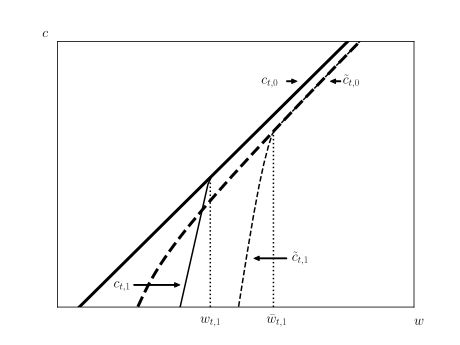
\includegraphics[width=.95\textwidth]{\FigDir/ConsWithWithoutConstrAndRisk}}

\caption{Consumption Functions with and without a Constraint and a Risk}
{\footnotesize \begin{singlespace} {\emph{Notes:} $c_{t,0}$ is the consumption function with no constraint and no risk, $\tilde{c}_{t,0}$ is the consumption function with no constraint and a risk that is realized between period $t$ and $t+1$, $c_{t,0}$ is the consumption function with one constraint in period $t+1$ and no risk, and $c_{t,0}$ is the consumption function with one constraint in period $t+1$ and a risk that is realized between period $t$ and $t+1$. The figure illustrates that the vertical distance between $c_{t,1}$ and $\tilde{c}_{t,1}$ is always greater than the vertical distance between $c_{t,0}$ and $\tilde{c}_{t,0}$ for $w < \bar{\omega}_{t,1}$. }  \end{singlespace}}
\label{fig:SolveConstrCompare4Cases}
\end{figure}
The darker loci reflect behavior of consumers who do not face the
future constraint, and the dashed loci reflect behavior of consumers
who \textit{do} face the immediate risk.  As expected, for levels of
wealth above $\wAlt_{t,1}$ where the future constraint
stops impinging on current behavior for perfect foresight consumers,
behavior of the constrained and unconstrained perfect foresight
consumers is the same. Similarly, $\tilde{c}_{t,1}(w_{t}) =
\tilde{c}_{t,0}(w_{t})$ for levels of wealth above ${\bar{\wAlt}}_{t,1}$
beyond which the probability of the future constraint binding is zero.
And for both constrained and unconstrained consumers, the introduction
of the risk reduces the level of consumption (the dashed loci are
below their solid counterparts). The importance of Theorem \ref{thm:riskandconstraints} in this context is that for levels of wealth below ${\bar{\wAlt}}_{t,1}$, the vertical distance between the solid and the dashed loci is greater for the constrained (thin line) than for the unconstrained (thick line) consumers, because of the interaction between the liquidity constraint and the precautionary motive.


%%%Thus, we can state a more general version of
%%%lemma~\ref{lemma:SolveConstrCompare4Cases},
%%%\input lemmaSolveConstrCompare4CasesMoreGen

%%%Finally, if there are no constraints that could apply, or risks that
%%%could be realized, between period $s < t$ and period $t$, it is
%%%simple to extend this to period $s$; we state this final
%%%version as a theorem,
%%%\begin{theorem}\label{thm:SolveConstrCompare4Cases}
%%%  Consider a consumer in period $s<t$ facing a set of liquidity
%%%  constraints $\mathcal{T}_{s} = \mathcal{T}_{t}$, and a
%%%  risk $\zeta_{t+1}$ that will be realized between the end of period $t$
%%%  and the beginning of period $t+1$.  The introduction of the risk
%%%  $\zeta_{t+1}$ has a larger precautionary effect on the level of
%%%  consumption (induces more precautionary saving) in period $s$ for a
%%%  consumer who faces the first $n+1$ liquidity constraints in
%%%  $\mathcal{T}_{s}$ than for a consumer who faces only the first
%%%  $n$ constraints.  That is,
%%%\begin{equation}
%%%  c_{s,n+1}(w_s) - \tilde{c}_{s,n+1}(w_s) \geq c_{s,n}(w_s)-\tilde{c}_{s,n}(w_s), \label{eq:nineqs}
%%%\end{equation}
%%%and the inequality is strict at levels of wealth
%%%$\tilde{\underline{\wAlt}}_{s,n+1} < w < \tilde{\bar{\wAlt}}_{s,n+1}$, where
%%%$\tilde{\underline{\wAlt}}_{s,n+1}$ (resp. $\tilde{\bar{\wAlt}}_{s,n+1}$) is the
%%%level of wealth such that a consumer in period $s$ with wealth
%%%$w_{s}=\tilde{\underline{\wAlt}}_{s,n+1}$ (resp.
%%%$w_{s}=\tilde{\bar{\wAlt}}_{s,n+1}$) will arrive at the beginning of period
%%%$t$ with wealth $\tilde{\underline{\wAlt}}_{t,n+1}$ (resp.
%%%$\tilde{\bar{\wAlt}}_{t,n+1}$).  For the exponential and power utility cases,
%%%the inequality is also strict for $w_{s} \leq
%%%\tilde{\underline{\wAlt}}_{s,n+1}$, while in the quadratic utility case \eqref{eq:nineqs}
%%%holds with equality for $w_{s} \leq
%%%\tilde{\underline{\wAlt}}_{s,n+1}.$
%%%\end{theorem}
%%%
%%%In intuitive terms, this theorem says that the precautionary saving induced
%%%by the introduction of the risk $\zeta_{t+1}$ is greater for the consumer
%%%facing $n+1$ constraints than for the consumer facing $n$ constraints
%%%at levels of wealth at which there is some probability that the $n+1$'th
%%%constraint will actually bind.
%%%
%%%The easiest way to see that the theorem holds (given the lemma) is to
%%%realize that in an unconstrained perfect foresight model behavior in
%%%period $s<t$ can be reformulated to combine multiple periods into one.
%%%Thus, for example, for CRRA utility, consumption two periods earlier
%%%can be obtained via the Euler equation from consumption one period
%%%earlier, and so on.  This means that the foregoing logic can be
%%%directly reinterpreted with appropriate substitutions of $s$ for $t$
%%%and appropriate reformulation of the dynamic budget constraint.


\subsection{A More General Result?}
The results in Theorem \ref{thm:riskandconstraints} is limited to the effects of an additional constraint when a household faces income risk that is realized between period $t$ and $t+1$. We could hope to find a more general result where precautionary saving increases if we for example impose an immediate constraint or an earlier risk, or generally multiple constraints or risks. However, it turns out that the answer is "not necessary" to all these possible scenarios. In this subsection, we argue for why we cannot derive more general results.

%%%\subsubsection{Earlier Risks and Constraints}\label{subsubsec:EarlierRisks}

%%%\ifthenelse{\boolean{Outline}}{
%%%\immediate{\write18{echo "...." EarlierRisks >> ./Index.txt}}}{}



 To examine these results, we need to develop a last bit of notation.  We define, $c_{t,n}^{m}$, as the consumption function in period $t$ assuming that the first $n$ constraints and the first $m$ risks have been imposed, counting risks, like constraints, backwards from period $T$.  Thus, relating our new notation to our previous usage, $c_{t,n}^{0}=c_{t,n}$ because 0 risks have been imposed. All other functions are defined correspondingly, e.g. $\Omega_{t,n}^{m}$ is the end-of-period-$t$ value function assuming the first $n$ constraints and $m$ risks have been imposed. We will continue to use the notation $\tilde{c}_{t,n}$ to designate the effects of imposition of a single immediate risk (realized between periods $t$ and $t+1$).

%%%Finally, we need to introduce a counter that keeps track of how many future risks exist beyond a given date, analogous to our $k_{t}$ counter that tells how many constraints exist after period $t$.  Call the risk-counter $q_{t}$.

Suppose now there are $m$ future risks that will be realized between $t$ and $T$. One might hope to show that the precautionary effect of imposing all risks in the presence of all constraints would be greater than the effect of imposing all risks in the absence of any
constraints:
\begin{equation}
  c_{t,n}^{0}(w) - c_{t,n}^{m}(w) \geq c_{t,0}^{0}(w) - c_{t,0}^{m}(w).\label{eq:nottrue}
\end{equation}
Such a hope, however, would be in vain.  In fact, we will now show that even the considerably weaker condition, involving only the single risk $\zeta_{t+1}$ and all constraints, $c_{t,n}^{0}(w) - c_{t,n}^{1}(w) \geq c_{t,0}^{0}(w) - c_{t,0}^{1}(w),$ can fail to hold for some $w$.


\subsubsection{An Immediate Constraint}\label{subsubsec:ImmediateConstr}


Consider a situation in which $n$ constraints applies in between $t$ and $T$.
%%%$\mathcal{T}_{t}[k_{t}]=T-t$; that
%%%is, the chronologically earliest constraint in $\mathcal{T}_{t}$
%%%applies at the end of period $t$.
Since $c_{t,n-1}$ designates the consumption rule that will be optimal prior to imposing the period-$t$ constraint, the consumption rule imposing all
constraints will be
%%%\begin{eqnarray}
%%%  c^{1}_{t,k_{t}}(w) & = & \min[c^{1}_{t,k_{t+1}}(w),w].
%%%\end{eqnarray}
\begin{eqnarray}
c_{t,n}(w) & = & \min[c_{t,n-1}(w),w].
\end{eqnarray}
Now define the level of wealth below which the period $t$ constraint binds for a consumer not facing the risk as ${\wAlt}_{t,n}.$ For values of wealth $w \geq {\wAlt}_{t,n},$ analysis of the effects of the risk is identical to analysis in the previous subsection where the first $n-1$ constraints were imposed. For levels of wealth $w < {\wAlt}_{t,n}$, we have $c^{1}_{t,n}(w) = c_{t,n}(w)=w$ (for the simple $c \leq w$
constraint; a corresponding point applies to the more sophisticated form of constraint); that is, for consumers with wealth below ${\wAlt}_{t,n}$, the introduction of the risk in period $t+1$ has no effect on consumption in $t$, because for these levels of wealth the constraint at the end of $t$ has the effect of `hiding' the
risk from view (they were constrained before the risk was imposed and remain constrained afterwards). Thus for households for whom inequality \eqref{eq:ineq} in Theorem \ref{thm:riskandconstraints} holds strictly in the absence of the constraint at $t$, at levels of wealth below ${\wAlt}_{t,n}$, the precautionary effect of the risk is wiped out.
%%% (For quadratic consumers, precautionary saving is zero for wealth below $\underline{\wAlt}^{1}_{t,N}$ both before and after the risk is imposed).

\begin{Private}
  \begin{comment} % This point is not really necessary; the objective here is to illustrate the point that with a constraint it is possible that the risk does nothing
  Finally, consider levels of wealth $\underline{\wAlt}^{1}_{t,k_{t}} < w <
  \wAlt_{t,k_{t}}.$ Since
  Theorem~\ref{thm:SolveConstrCompare4Cases} holds as a strict
  inequality for exponential and CRRA consumers at $w=\wAlt_{t,k_{t}}$
  but fails at $w=\underline{\wAlt}^{1}_{t,k_{t}}$ because the unconstrained
  consumer has positive precautionary saving but the constrained one
  does not, there will be some intermediate value of wealth at which
  the the proposition just stops holding (since both consumption
  functions are continuous, the intermediate value Theorem applies).
\end{comment}
\end{Private}

\subsubsection{An Earlier Risk}\label{subsubsec:AnEarlierRisk}


Consider now the question of how the addition of a risk $\zeta_{t}$ that will be realized between periods $t-1$ and $t$ affects the consumption function at the beginning of period $t-1$, in the absence of any constraint at the beginning of period $t$.

The question at hand is then whether we can say that
\begin{eqnarray}
  \label{eq:earlierrisk}
  c_{t-1,0}^{1}(w)-c_{t-1,0}^{2}(w) & \geq & c_{t-1,0}^0(w)-c^{1}_{t-1,0}(w);
\end{eqnarray}
that is, does the introduction of the risk $\zeta_{t}$ have a greater precautionary effect on consumption in the presence of the subsequent risk $\zeta_{t+1}$ than in its absence?

The answer again is ``not necessarily.''  To see why, we present an example in Appendix \ref{app:similar} of a CRRA utility problem in which in a certain limit the introduction of a risk produced an effect on the consumption function that is indistinguishable from the effect of a liquidity constraint.  If the risk $\zeta_{t}$ is of this liquidity-constraint-indistinguishable form, then the logic of the previous subsection clearly applies: For some levels of wealth, the introduction of the risk at $t$ can `hide' the precautionary effect of any risks at $t+1$ or later.

\subsection{What Can Be Said?}\label{subsubsec:WhatCanBeSaid}



It might seem that the previous subsection implies that little useful can be said about the precautionary effects of introducing a new risk in the presence of preexisting constraints and risks. It turns out, however, that there is at least one useful result.

\begin{theorem}\label{thm:CCandPS}
	Consider an agent who has a utility function with $u'> 0$, $u''< 0$, $u''' > 0$, and non-increasing absolute prudence $-u'''/u''$. Then the introduction of a risk $\zeta_{t+1}$ has a greater precautionary effect on level $t$ consumption in the presence of all future risks and constraints than in the absence of any future risks and constraints, i.e.
	\begin{eqnarray}
	c_{t,n}^{m-1}(w) - c_{t,n}^{m}(w) & > & c_{t,0}^0(w)-c^{1}_{t,0}(w) \label{eq:whatcanbesaid}
	\end{eqnarray}
	%the introduction of the risk $\zeta_{\tau+1}$ has a larger (precautionary) effect on the level of period-$\tau$ consumption in the presence of all future risks and constraints than in absence of any future risks and constraints
	at levels of period-$t$ wealth $w$ such that in the absence of the new risk the consumer is not constrained in the current period $(c_{t,n}^{m-1}(w) > w)$ and in the presence of the risk there is a positive probability that some future constraint will bind.
%%% 	\begin{enumerate}
%%% 		\item if utility is quadratic, there is some future constraint such that the probability that it binds depends on the value of $\zeta_{t+1}$ that is realized.
%%% 		\item if utility is exponential, there is a positive probability that some future constraint will bind.
%%% 		\item if utility is CRRA, there is a positive probability that some future constraint will bind, or the initial situation is one in which there is some nondegenerate future risk.
%%% 	\end{enumerate}
\end{theorem}

Appendix \ref{app:CCandPS} presents the proof. It seems to us that a fair summary of this theorem is that in most circumstances the presence of future constraints and risks does increase the amount of precautionary saving induced by the introduction of a given new risk.  The primary circumstance under which this should not be expected is for levels of wealth at which the consumer was constrained even in the absence of the new risk. There is no guarantee that the new risk will produce a sufficiently intense precautionary saving motive to move the initially-constrained consumer off his constraint.  If it does, the effect will be precautionary, but it is possible that no effect will occur.

\end{verbatimwrite}\ifVerbatimWrite{\input{Sections/LCandPS}}{} %%% Private

\section{Conclusion}

The central message of this paper is that the effects of precautionary saving and of liquidity constraints are very similar to each other, because the introduction of either a liquidity constraints or of a risk induce counterclockwise concavifications of the consumption function. This increase in concavity increases prudence and induces households to save more for precautionary reasons. 

In addition, we provide an explanation of the apparently contradictory results that have emerged from simulation studies, which have sometimes seemed to indicate that constraints intensify precautionary saving motives, and sometimes have found constraints and precautionary behavior to be substitutes. The insight here is that the outcome depends on whether the introduction of a constraint or risk hides any previous constraints or risks. If the new constraint or risks does not hide existing constraints or risks, it intensifies the precautionary saving motive. If it hides any existing constraints or risks, it might weaken the precautionary saving motive.  

%%% Our results may have important applications even beyond the 
%%% traditional consumption/saving problem in which the results were 
%%% derived.  The precautionary-saving effect of liquidity constraints may 
%%% apply in many circumstances where a decision-maker faces the 
%%% possibility of future liquidity constraints which raise the 
%%% marginal value of an extra dollar of cash.  Thus, firms that are not 
%%% currently liquidity constrained may engage in precautionary saving if 
%%% they believe there is some risk that constraints may bind in the 
%%% future.  Governments that worry about whether they will always be able 
%%% to borrow on international markets may engage in precautionary saving 
%%% even in periods when they are unconstrained.  The logic could even 
%%% apply to central banks charged with the responsibility of maintaining 
%%% stable exchange rate regimes; the possibility of a run on the currency 
%%% might induce `precautionary' holdings of international reserves that 
%%% are larger than a risk-neutral central bank would hold.  Of course, 
%%% these are all ideas that have appeared, at least informally and 
%%% sometimes formally, in the relevant literatures.  But this 
%%% paper provides a general logic which can be applied to clarify 
%%% precisely when and why one should expect such effects to emerge.

\bibliography{LiqConstr,economics}

\vfill\eject
\appendix


%%% \section{Proof of Theorem \ref{thm:riskandconstraints}}
%%%\subfile{Sections/Proofs}
%%%\end{onehalfspace}

\begin{verbatimwrite}{Sections/Proofs} %%% Private
  
\section{Proof of Lemma \ref{lem:counterclockwise}} \label{app:counterclockwise}
\begin{proof} First, condition 2 and 4 in Definition \ref{defn:cconcavification} implies that $\hat{c}'(w) > c'(w)$ for $w = w^{\#} - \epsilon$ for a small $\epsilon > 0$. Condition 3 then ensures that $\lim_{\upsilon \uparrow w} \hat{c}'(\upsilon) > \lim_{\upsilon \uparrow w} c'(\upsilon)$ holds for all $w \leq w^{\#}-\epsilon$ (equivalently $w < w^{\#}$). Second, condition 1 and the fact that $\lim_{\upsilon \uparrow w} \hat{c}'(\upsilon) > \lim_{\upsilon \uparrow w} c'(\upsilon)$ for $w < w^{\#}$ implies that $\lim_{\upsilon \uparrow w} \hat{c}(\upsilon) < \lim_{\upsilon \uparrow w}c(\upsilon)$ for $w < w^{\#}$. Third, condition 2 in Definition \ref{defn:cconcavification} implies that $$\lim_{\upsilon \uparrow w}\hat{c}''(\upsilon) \leq \lim_{\upsilon \uparrow w} c''(\upsilon)\frac{\hat{c}'(\upsilon)}{c'(\upsilon)}$$ for $w < w^{\#}$. Then $$\lim_{\upsilon \uparrow w} \hat{c}''(\upsilon) \leq \lim_{\upsilon \uparrow w} c''(\upsilon)$$ since $\lim_{\upsilon \uparrow w}\hat{c}'(\upsilon) > \lim_{\upsilon \uparrow w} c'(\upsilon)$ for $w < w^{\#}$. Note that the inequality is not strict since $c''(\upsilon)$ could be 0.  
\end{proof}



\section{Proof of Theorem \ref{thm:CCToPrud}} \label{app:CCToPrud}
\begin{proof}
	By the envelope theorem, we know that 
	\[ V'(w) = u'(c(w))\]
	Differentiating with respect to $w$ yields\footnote{Since $c(w)$ is concave, it has left-hand and right-hand derivatives at every point, though the left-hand and right-hand derivatives may not be equal. Equation \eqref{eq:diff2} should be interpreted as applying the left-hand and right-hand derivatives separately. (Reading \eqref{eq:diff2} in this way implies that $c'(w^-) \geq c'(w^+)$; therefore $V''(w^-) \leq V''(w^+)$).}
	\begin{equation}\label{eq:diff2}
	V''(w) = u''(c(w))c'(w)
	\end{equation}
	Taking another derivative can run afoul of the possible discontinuity in $c'(w)$ that we will show below can arise from liquidity constraints. We therefore consider two cases: (i) $c''(w)$ exists and (ii) $c''(w)$ does not exist. 
	
	\bigskip
	\noindent \textbf{\textit{Case I:}} ($c''(w)$ exists).\\
	In the case where $c''(w)$ exists, we can take another derivative
	\[V'''(w) = u'''(c(w))[c'(w)]^2 + u''(c(w))c''(w)\]
	Absolute prudence of the value function is thus defined as
	\begin{align}-\frac{V'''(w)}{V''(w)} &= -\frac{u'''(c(w))[c'(w)]^2 + u''(c(w))c''(w)}{u''(c(w))c'(w)} \nonumber \\
	-\frac{V'''(w)}{V''(w)} &= -\frac{u'''(c(w))}{u''(c(w))}c'(w) - \frac{c''(w)}{c'(w)}\label{eq:absprudence}\end{align}
	From the assumption that $\hat{c}(w)$ is a counterclockwise concavification of $c(w)$, we know from Lemma \ref{lem:counterclockwise} that  $\hat{c}(w) \leq c(w)$ and $\hat{c}'(w) \geq c'(w)$. Furthermore, since $-\frac{u'''(c(w))}{u''(c(w))}$ is non-increasing, we know that $-\frac{u'''(\hat{c}(w))}{u''(\hat{c}(w))} \geq -\frac{u'''(c(w))}{u''(c(w))}$. As a result, $-\frac{u'''(\hat{c}(w))}{u''(\hat{c}(w))}\hat{c}'(w) \geq -\frac{u'''(c(w))}{u''(c(w))}c'(w)$. 
	
	The second part of the absolute prudence expression, $-\frac{c''(w)}{c'(w)}$, is a measure of the curvature of the consumption function. Since the consumption function is concave, it is then a measure of the degree of concavity. Formally, if we have two functions, $f(x)$ and $g(x)$, that both are increasing and concave functions, then the concave transformation $g(f(x))$ always has more curvature.\footnote{To see this, calculate \[-\frac{\frac{d^2}{dx^2} g(f(x))}{\frac{d}{dx}g(f(x))} = - \frac{g''f'}{g'} - \frac{f''}{f'} \geq - \frac{f''}{f'}\] where the inequality holds since $g' \geq 0$ and $g'' \leq 0$.} A counterclockwise concavification is an example of such a $g$. Hence, $-\frac{\hat{c}''(w)}{\hat{c}'(w)} \geq -\frac{c''(w)}{c'(w)}$. Then
	\begin{align*}
	-\frac{\hat{V}'''(w)}{\hat{V}''(w)} &= -\frac{u'''(\hat{c}(w))}{u''(\hat{c}(w))}\hat{c}'(w) - \frac{\hat{c}''(w)}{\hat{c}'(w)} \\ 
	&\geq -\frac{u'''(c(w))}{u''(c(w))}c'(w) - \frac{c''(w)}{c'(w)} = -\frac{V'''(w)}{V''(w)}
	\end{align*}
%%%	Even when absolute prudence of the utility function is constant, the inequality is strict whenever $\hat{c}$ is strictly more concave at some level of wealth at or above $w$ since with weak concavity everywhere, strictly more concave anywhere above $w$ implies that $\hat{c}'(w) > c'(w)$. 
	
	\bigskip
	\noindent \textbf{\textit{Case II:}} ($c''(w)$ does not exist).\\
	Informally, if nonexistence is caused by a constraint binding at $w$, the effect will be a discrete decline in the marginal propensity to consume at $w$, which can be thought of as $c''(w) = -\infty$, implying positive infinite prudence at that point (see \eqref{eq:absprudence}). Formally, if $c''(w)$ does not exist, greater prudence of $\hat{V}$ than $V$ is defined as $\frac{\hat{V}''(w)}{V''(w)}$ being a decreasing function of $w$. This is defined as
	\[\frac{\hat{V}''(w)}{V''(w)} \equiv 
	\left(\frac{u''(\hat c(w))}{u''(c(w))} \right)
	\left(\frac{\hat{c}'(w)}{c'(w)}\right)\]
	The second factor, $\frac{\hat{c}'(w)}{c'(w)}$, is weakly decreasing in $w$ by the assumption of counterclockwise concavity. At any specific value of $w$ where
	$\hat{c}''(w)$ does not exist because the left and right hand
	values of $\hat{c}'$ are different, we say that $\hat{c}'$
	is decreasing if
	\begin{eqnarray}
	\lim_{w^{-} \rightarrow w} \hat{c}'(w) & > & \lim_{w^{+} \rightarrow w} \hat{c}'(w).
	\end{eqnarray}
	
	As for the first factor, note that nonexistence of
	$\hat{V}'''(w)$ and/or $\hat{c}''(w)$ do not
	spring from nonexistence of either $u'''(c)$ or $\lim_{w \uparrow
		w} \hat{c}'(w)$ (for our purposes, when the
	left and right derivatives of $\hat{c}(w)$ differ at a point, the
	relevant derivative is the one coming from the left; rather than carry
	around the cumbersome limit notation, read the following derivation as
	applying to the left derivative).  To discover whether $\frac{\hat
		{V}''(w)}{V''(w)}$ is decreasing we can simply
	differentiate:
	\begin{align*}
	\frac{d}{d w}\left( \frac{u''(\hat{c}(w))}{ u''(c(w))}\right) &=& \frac{u'''(\hat{c}(w))\hat{c}'(w)u''(c(w))-u''(\hat{c}(w))u'''(c(w))c'(w)}{[u''(c(w))]^{2}}. \qquad \qquad
	\end{align*}
	
	Since the denominator is always positive, this will be negative if the 
	numerator is negative, i.e.  if
	\begin{align}
	u'''(\hat{c}(w))u''(c(w))\hat{c}'(w) & \leq  u''(\hat{c}(w))u'''(c(w))c'(w) \nonumber
	\\  \frac{u'''(\hat{c}(w))}{u''(\hat{c}(w))}\hat{c}'(w) & \leq  \frac{u'''(c(w))}{u''(c(w))}c'(w) \nonumber
	\\  -\frac{u'''(\hat{c}(w))}{u''(\hat{c}(w))}\hat{c}'(w) & \geq  -\frac{u'''(c(w))}{u''(c(w))} c'(w) \label{eq:prudcond} .
	\end{align}
	
	Recall from Lemma \ref{lem:counterclockwise} that $\hat{c}'(w) \geq c'(w)$ and $\hat{c}(w) \leq c(w)$ so non-increasing absolute prudence of the utility function ensures that $-\frac{u'''(\hat{c}(w))}{u''(\hat{c}(w))} \geq  -\frac{u'''(c(w))}{u''(c(w))}$. Hence both terms on the LHS are greater than or equal to the corresponding terms on the RHS of equation \eqref{eq:prudcond}. 
	% The inequality is strict at any point for which $\hat{c}'(w) > c'(w)$.
	
	%Note finally that condition \eqref{eq:prudcond} is equivalent to
	%our definition of property greater CC for consumption functions for
	%which $c'(w)$ and $\hat{c}'(w)$ exist in the sense of
	%left and right derivatives. 
	%
	%Thus, combining all of the factors involved in comparing the prudence
	%of $\hat{V}(w)$ to the prudence of $V(w)$, we have
	%shown that the value function in the modified situation will exhibit
	%strictly greater prudence at any given $w$ than the value function
	%in the baseline situation if and only if $\hat{c}(w)$ is
	%strictly concave at $w$ or at some level of wealth above $w$.
	
\end{proof}



\section{Proof of Corollary \ref{cor:ccandstrictprud}} \label{app:ccandstrictprud}
\begin{proof}
	We prove each statement in Corollary \ref{cor:ccandstrictprud} separately. 
	
	\bigskip
	\noindent \textbf{\textit{Case I:}} ($ u ''' > 0$). \\
	If $u''' > 0$, a counterclockwise concavification around $w^{\#}$ implies that $\hat{c}(w) < c(w)$ and $\hat{c}'(w) > c'(w)$ for all $w < w^{\#}$. Then \[-\frac{u'''(\hat{c}(w))}{u''(\hat{c}(w)}\hat{c}'(w) > -\frac{u'''({c}(w))}{u''({c}(w))}{c}'(w) \text{ for } w < w^{\#} \]
	Since we know that \[-\frac{\hat{c}''(w)}{\hat{c}'(w)} \geq -\frac{{c}''(w)}{{c}'(w)} \text{ for } w < w^{\#}\]
	from the proof of Theorem \ref{thm:CCToPrud}, we know that
	\begin{align*}- \frac{\hat{V}'''(w)}{\hat{V}''(w)} &= -\frac{u'''(\hat{c}(w))}{u''(\hat{c}(w)}\hat{c}'(w) - \frac{\hat{c}''(w)}{\hat{c}'(w)}
	\\
	& > -\frac{u'''({c}(w))}{u''({c}(w))}{c}'(w) - \frac{{c}''(w)}{{c}'(w)} = - \frac{{V}'''(w)}{{V}''(w)} \text{ for } w < w^{\#}
	\end{align*}
	
	\bigskip
	\noindent \textbf{\textit{Case II:}} ($u''' = 0$). \\
	The quadratic case requires a different approach. Note first that the conditions in Corollary \ref{cor:ccandstrictprud} hold only below the bliss point for quadratic utility. In addition, since $u'''(\cdot) = 0$, strict inequality between the prudence of $\hat{V}$ and the prudence of $V$ hold only at those points where $\hat{c}(\cdot)$ is strictly concave. 
	
	Recall from the proof of Theorem \ref{thm:CCToPrud} that greater prudence of $\hat{V}(w)$ than $V(w)$ occurs if  $\frac{\hat{V}''(w)}{V''(w)}$ is decreasing in $w$. In the quadratic case
	\begin{equation}
	\frac{\hat{V}''(w)}{V''(w)} = \frac{u''(\hat{c}(w))}{u''(c(w))} \frac{\hat{c}'(w)}{c'(w)} = \frac{\hat{c}'(w)}{c'(w)}
	\end{equation}
	where the second equality follows since $u''(\cdot)$ is constant with quadratic utility. Thus, prudence is strictly greater in the modified case only if $ \frac{\hat{c}'(w)}{c'(w)}$ strictly declines in $w$.
\end{proof}

\section{Proof of Theorem \ref{thm:recursive}}\label{app:recursive}

\begin{proof}
	First, to facilitate readability of the proof, we assume that $R = \beta = 1$ with no loss of generality. Our goal is to prove that $V(w_t) \in CC$ if $V_{t+1}(s_t + {y}_{t+1}) \in CC$ for all realization of ${y}_{t+1}$. The proof proceeds in two steps. First, we show that property CC is preserved through the expectation operator (vertical aggregation),
	\[\Omega(s_t) = \Ex_t[V_{t+1}(s_t + {y}_{t+1})] \in CC,\]
	whenever $V_{t+1}(s_t + {y}_{t+1}) \in CC$ for all realization of ${y}_{t+1}$. Second, we show that property CC is preserved through the value function operator (horizontal aggregation),
	\[V(w_t) = \max_{s} u(c_t(w_t - s)) + \Omega(s) \in CC, \]
	whenever $\Omega(s) \in CC$. Throughout the proof, the first order condition holds with equality since no liquidity constraint applies at the end of period $t$. 
	
	\bigskip
	\noindent \textbf{Step 1: Vertical aggregation} \\ 
	%%%%%%%%%%%%%%%%%%%%%%%%%%%%%%%%%%%%%%%%%%%%%%%%%%%%%%%%
	\noindent We show that consumption concavity is preserved under vertical aggregation for three cases of the HARA utility function with $u''' \geq 0$ ($a \geq -1$) and non-increasing absolute prudence ($a \notin (-1,0)$). The three cases are
	\begin{equation}\label{eq:HARAmu}u'(c) = \begin{cases} \left(ac + b\right)^{-1/a} & a > 0 \text{ (CRRA)} \\
	e^{-c/b} & a = 0 \text{ (CARA)}\\
	ac + b & a = -1 \text{ (Quadratic)}\end{cases} \end{equation}
	
	\bigskip
	\noindent \textbf{Case I ($a > 0$, CRRA).} 	We will show that concavity is preserved under vertical aggregation for $c^{-1/a}$ to avoid clutter, but the results hold for all affine transformations, $ac + b$, with strictly positive $a$. Concavity of $c_{t+1}(s_t + \chi{y}_{t+1})$ implies that
	\begin{equation}c_{t+1}(s_t + {y}_{t+1}) \geq pc_{t+1}(s_1 + {y}_{t+1}) + (1-p) c_{t+1}(s_2 + {y}_{t+1}) \label{eq:vert_crra_conc}\end{equation}
	for all ${y}_{t+1} \in [\underline{y},\bar{y}]$ if $s_t = ps_1 + (1-p)s_2$ with $p \in [0,1]$. Since this holds for all ${y}_{t+1}$, we know that
	\[\left\{\Ex_t\left[c_{t+1}(s_t + \chi{y}_{t+1})^{-\frac{1}{a}}\right]\right\}^{-a} \geq \left\{\Ex_t\left[\left\{pc_{t+1}(s_1 + \chi{y}_{t+1}) + (1-p) c_{t+1}(s_2 + \chi{y}_{t+1})\right\}^{-\frac{1}{a}}\right]\right\}^{-a}\]
	
	By Minkowski's inequality, we know that for $a > 0$ $(a > -1, a \neq 0)$
	\[\left\{\Ex[(u + v)^{-\frac{1}{a}}]\right\}^{-a} \geq \left\{\Ex[u^{-\frac{1}{a}}]\right\}^{-a} + \left\{\Ex[v^{-\frac{1}{a}}]\right\}^{-a}\]
	if $u\geq 0$ and $v\geq 0$. Thus
	\begin{align*}
	&\left\{ \Ex_t \left[\left\{pc_{t+1}(s_1 + \chi{y}_{t+1}) + (1-p) c_{t+1}(s_2 + \chi{y}_{t+1})\right\}^{-\frac{1}{a}}\right]\right\}^{-a} \\ & \geq \left\{ \Ex_t \left[\left\{pc_{t+1}(s_1 + \chi{y}_{t+1})\right\}^{-\frac{1}{a}}\right]\right\}^{-a} + \left\{ \Ex_t \left[\left\{(1-p) c_{t+1}(s_2 + \chi{y}_{t+1})\right\}^{-\frac{1}{a}}\right]\right\}^{-a} \\
	& = p\left\{ \Ex_t \left[\left\{c_{t+1}(s_1 + \chi{y}_{t+1})\right\}^{-\frac{1}{a}}\right]\right\}^{-a} +(1-p) \left\{ \Ex_t \left[\left\{ c_{t+1}(s_2 + \chi{y}_{t+1})\right\}^{-\frac{1}{a}}\right]\right\}^{-a} \\ & = p(\Omega'(s_1))^{-a} + (1-p)(\Omega'(s_2))^{-a}
	\end{align*}
	which implies that 
	\[ (\Omega'(s_t))^{-a} \geq p(\Omega'(s_1))^{-a} + (1-p)(\Omega'(s_2))^{-a}\]
		
%%%	is strict unless
%%%	$c_{t+1}(s_{2}+\chi{y}_{t+1})/c_{t+1}(s_{1}+\tilde{y}_{t+1})$ is a constant for all realizations of $\tilde{y}_{t+1}$.  But for this to be true for any $s_{1}$ and $s_{2}$ it must be the case that
%%%	\begin{align*}
%%%	\left(\frac{d}{d s_{2}}\right)\left(\frac{c_{t+1}(s_{2}+\tilde{y}_{t+1})}{c_{t+1}(s_{1}+\tilde{y}_{t+1})}\right) \Bigg\vert_{s_2 = s_1} & = & \left(\frac{c_{t+1}^{'}(s_{1}+\tilde{y}_{t+1})}{c_{t+1}(s_{1}+\chi{y}_{t+1})}\right) = \nu
%%%	\end{align*}
%%%	for some constant $\nu$. However, this is only true if the consumption function is $c_{t+1}(w) = \exp(\nu w)$, which is not true.
	Thus, defining
	$\chi_{t}(s_{t}) = \{\Omega_{t}^{'}(s_{t})\}^{-a}$, we get
	\begin{align*}
	\chi_{t}(s_{t}) \geq p \chi_{t}(s_{1}) + (1-p) \chi_{t}(s_{2})
	\end{align*}
	for all $s_{t}$, where the inequality is strict if $c_{t+1}$ is strictly concave for at least one realization of ${y}_{t+1}$.
	
	\bigskip
	\noindent \textbf{Case II ($a = 0$, CARA)}. For the exponential case, property CC holds at $s_{t}$ if 
	\begin{eqnarray*}
	\exp(-\chi_{t}(s_{t})/b) & = & \Ex_{t}[ \exp(-c_{t+1}(s_{t}+{y}_{t+1})/b)]
	\end{eqnarray*}
	for some $\chi_{t}(s_{t})$ which is strictly concave at $s_{t}$. We set $b = 1$ to reduce clutter, but results hold for $b \neq 1$. Consider first a case where $c_{t+1}$ is linear over the range of possible values of $s_{t}+{y}_{t+1}$, then 
	\begin{eqnarray}
	\chi_{t}(s_{t}) & = & -\log \Ex_{t}[e^{-c_{t+1}(s_{t}+{y}_{t+1})}] \nonumber 
	\\& = & -\log \Ex_{t}[e^{-(c_{t+1}(s_{t}+\bar{y})+({y}_{t+1}-\bar{y})c_{t+1}^{'})}] \nonumber
	\\ & = & c_{t+1}(s_{t}+\bar{y}) - \log \Ex_{t}[e^{-({y}_{t+1}-\bar{y}) c_{t+1}^{'}}] \label{eq:expcdrops}
	\end{eqnarray}
	which is linear in $s_{t}$ since the second term is a constant.  
	
	Now consider a value of $s_{t}$ for which $c_{t+1}(s_{t}+{y}_{t+1})$ is strictly concave for at least one realization of ${y}_{t+1}$. Global weak concavity of $c_{t+1}$ tells us that for every ${y}_{t+1}$
	\begin{eqnarray}
	-c_{t+1}(s_{t}+{y}_{t+1}) & \leq & -((1-p)c_{t+1}(s_1+{y}_{t+1})+pc_{t+1}(s_{2}+{y}_{t+1})) \nonumber
	\\ \Ex_{t}[e^{-c_{t+1}(s_{t}+{y}_{t+1})}] & \leq & \Ex_{t}[e^{-((1-p)c_{t+1}(s_1+{y}_{t+1})+pc_{t+1}(s_{2}+{y}_{t+1}))}]. \label{eq:expconc}
	\end{eqnarray}
	
	Meanwhile, the arithmetic-geometric mean inequality states that for
	positive $u$ and $v$, if $\bar u = \Ex_t [ u]$ and $\bar v = \Ex_t [ v]$, then
	\begin{equation*}
	\Ex_t\left[( u/\bar u)^p ( v/\bar v)^{1-p}\right] 
	\leq \Ex_t \left[p ( u/\bar u)+(1-p)( v/\bar v)\right] = 1, 
	\end{equation*}
	implying that 
	\begin{equation*}
	\Ex_t [ u^p  v^{1-p}] \leq \bar u^p \bar v^{1-p}, 
	\end{equation*}
	where the expression holds with equality only if $v$ is proportional to $u$.  Substituting in $u= e^{-c_{t+1}(s_1 + {y}_{t+1})}$ and $v = e^{-c_{t+1}(s_2 + {y}_{t+1})}$, this means that
	\begin{eqnarray*}
	\Ex_t [e^{-p c_{t+1}(s_1 + {y}_{t+1}) - (1-p)c_{t+1}(s_2 + {y}_{t+1})}] & \leq &
	\left\{ \Ex_t  [e^{- c_{t+1}(s_1 + {y}_{t+1})} ] \right\}^p \left\{ \Ex_t  [e^{- c_{t+1}(s_2 + {y}_{t+1})} ] \right\}^{1-p}
	\end{eqnarray*}
	and we can substitute for the LHS from \eqref{eq:expconc}, obtaining
	\begin{eqnarray}
	\Ex_{t}[e^{-c_{t+1}(s_{t}+{y}_{t+1})}] & \leq &
	\left\{ \Ex_t  [e^{- c_{t+1}(s_1 + {y}_{t+1})} ] \right\}^p 	\left\{ \Ex_t  [e^{- c_{t+1}(s_2 + {y}_{t+1})} ] \right\}^{1-p} \nonumber
	\\ 
	\log \Ex_{t}[e^{-c_{t+1}(s_{t}+{y}_{t+1})}] &\leq &
	p \log \Ex_t  [e^{-c_{t+1}(s_1 + {y}_{t+1})} ] 
	+ (1-p) \log \Ex_t  [e^{-c_{t+1}(s_2 + {y}_{t+1})} ]  \label{eq:expineq2} 
	\end{eqnarray}
	which holds with equality only when
	$e^{-c_{t+1}(s_{1}+{y}_{t+1})}/e^{-c_{t+1}(s_{2}+{y}_{t+1})}$ is a constant. This will only happen if
	$c_{t+1}(s_{1}+{y}_{t+1})-c_{t+1}(s_{2}+{y}_{t+1})$ is constant, which (given that the MPC is strictly positive everywhere) requires
	$c_{t+1}(s_{t}+{y}_{t+1})$ to be linear for ${y}_{t+1} \in
	(\underline{y},\bar{y})$. Hence, 
	\begin{eqnarray*}
	\chi_{t}(s_t) & \geq & p \chi_{t}(s_{1}) + (1-p) \chi_{t}(s_{2}).
	\end{eqnarray*}
	where the inequality is strict for an $s_{t}$ from which $c_{t+1}$ is strictly concave for some realization of ${y}_{t+1}$.
	
	
	
%%%	Thus, in the exponential case, $\mathcal{S}_{t}$ includes any value of $s_{t}$ from which, for some point $w \in \mathcal{W}_{t+1}$, there is positive probability of arriving at a $w_{t+1} > w$ and a positive 	probability of arriving at a $w_{t+1} < w$. Formally,
%%%	\begin{equation}
%%%	\mathcal{S}_{t} =
%%%	\{s | s+\bar{y}+\zeta \in \mathcal{W}_{t+1} \}
%%%	\end{equation}
%%%	for some $\zeta \in [\underline{\zeta},\bar{\zeta}] $.  In words,
%%%	$\mathcal{S}_{t}$ is the set of values of $s$ from which the outcome
%%%	of the risk affects which side of $w$ the consumer ends up on for some
%%%	$w \in \mathcal{W}_{t+1},$ or from which there is a positive
%%%	probability of ending up exactly at
%%%	some $w \in \mathcal{W}_{t+1}$.
%%%	
	
	\bigskip
	\noindent \textbf{Case III ($a = -1$, Quadratic)}.
	In the quadratic case, linearity of marginal utility implies that
	\begin{eqnarray*}
	u'(\chi_{t}(s_{t})) & = & \Ex_{t}[u'(c_{t+1}(s_{t}+{y}_{t+1}))]
	\\   \chi_{t}(s_{t}) & = & \Ex_{t}[c_{t+1}(s_{t}+{y}_{t+1})]
	\end{eqnarray*}
	so $\chi_{t}$ is simply the weighted sum of a set of
	concave functions where the weights correspond to the probabilities of the various possible outcomes for ${y}_{t+1}$. The sum of concave functions
	is itself concave. And if additionally the consumption function is strictly concave at any point, the weighted sum is also strictly concave.
	
%%%	\bigskip
%%%	\noindent \textbf{Conclusion}.
%%%	Hence, we conclude that 
%%%	\begin{eqnarray*}
%%%		\chi_{t}(s_t) & \geq & p \chi_{t}(s_{1}) + (1-p) \chi_{t}(s_{2}).
%%%	\end{eqnarray*}
%%%	for all HARA utility functions with $u''' \geq 0$, and non-increasing absolute prudence. In addition, the inequality is strict for all values of $s_{t}$ where $c_{t+1}$ is strictly concave for at least one realization of ${y}_{t+1}$.
	
	
	
	
	
	%%%%%%%%%%%%%%%%%%%%%%%%%%%%%%%%%%%%%%%%%%%%%%%%%%%%%%%%%
	%%
	%%Assume that $V_{t+1}(w_{t+1}) \in CC$ for all $w_{t+1} \in [s_t + \underline{y}, s_t + \bar{y}_{t+1}]$. By the envelope theorem, we know that 
	%%\begin{align*}
	%%	u'(\chi(s_t)) &= \Omega'(s_t) \\ &= \Ex_t[V_{t+1}'(s_t + \tilde{y}_{t+1})] \\
	%%%	&= \int_{\underline{y}}^{\bar{y}_{t+1}} V'_{t+1} (s_t + y_t) dy \\
	%%%		& =
	%%%	V'_{t+1}(s_t + E(\tilde{y}_{t+1}) - \psi(s_t, \tilde{y}_{t+1})) \\ 
	%%%&= \int_{\underline{y}}^{\bar{y}_{t+1}}u'({c}_{t+1}(s_t + y_t))dy
	%%& = \Ex_t[u'(c_{t+1}(s_t + \tilde{y}_{t+1}))] 
	%%\end{align*}
	%%where $\psi(s_t + \tilde{y}_{t+1})$ is the equivalent precautionary premium with $\partial_s \psi(s_t,\tilde{y}_{t+1}) \leq 0$ since the utility function satisfies non-increasing absolute prudence $-u'''/u''$ \citep{kimball:smallandlarge}. %  $\partial_{ss} \psi(s_t,\tilde{y}_{t+1})\geq 0$ since $u''' \geq 0$. 
	%%Now since $u'$ is the same, we know that
	%%\[\chi(s_t) = (u')^{-1} \int_{\underline{y}}^{\bar{y}_{t+1}}u({c}_{t+1})dy = \int_{\underline{y}}^{\bar{y}_{t+1}}{c}_{t+1}(s_t + y_t)dy > 0\]
	%%since the integral is a sum. 
	%%From the envelope theorem, we also know that
	%%\begin{align}
	%%	u''(\chi(s_t))\chi'(s_t) =& \Ex_t[ u''(c_{t+1}){c}_{t+1}'(s_t + y_t )]  \nonumber \\
	%%	\chi'(s_t) =& \frac{\Ex_t[ u''(c_{t+1}){c}_{t+1}'(s_t + y_t )]}{u''(\chi(s_t))} > 0 
	%%	\end{align}
	%%	\begin{align}
	%%	u'''(\chi(s_t))\chi'(s_t)^2 + u''(\chi(s_t))\chi''(s_t) =& \Ex_t[ u'''(c_{t+1}){c}_{t+1}'(s_t + y_t)^2 + u''(c_{t+1}){c}_{t+1}''(s_t + y_t)]  \label{eq:VertConcave}
	%%\end{align}
	%%so $\chi(s_t)$ inherits all properties from ${c}_{t+1}$. Hence, $\Omega(s_t)$ has property CC when $V_{t+1}(w_{t+1})$ has property CC. 
	
	%%then 
	%%\[\Omega_t''(s_t) = \Ex_t [u''(c_{t+1})c_{t+1}'] < 0\]
	%%and
	%%\begin{equation}\Omega_t'''(s_t) = \Ex_t [u'''(c_{t+1})c_{t+1}'^2 + u''(c_{t+1})c_{t+1}''] \geq 0\label{eq:recursive1}\end{equation}
	%%since $u'> 0$, $u'' < 0$, and $u''' \geq 0$. 
	%%
	%%From the first order condition, we know that the consumption function corresponding to the expected value function is implicitly defined as 
	%%\[u'(\chi(s_t)) = \Omega'(s_t)\]
	%%Note that $\chi(s_t) \neq c_{t+1}(w_{t+1})$ since $\chi(s_t)$ is the consumption function corresponding to the expected value function (as if the future was certain). Differentiate both sides with respect to $s_t$ and obtain
	%%\[u''(\chi(s_t))\chi'(s_t) = \Omega''(s_t) \]
	%%Since $\Omega''(s_t) < 0$ and $u''(\chi(s_t)) < 0$, we have
	%%\[\chi'(s_t) = \frac{\Omega''(s_t)}{u''(\chi(s_t))} > 0\]
	%%and
	%%\begin{align} \chi''(s_t) &= \frac{\Omega'''(s_t)}{u''(\chi(s_t))} -\frac{\Omega''(s_t)u'''(\chi(s_t))\chi'(s_t)}{u''(\chi(s_t))^2}  \nonumber\\
	%%& = \frac{\Omega'''(s_t)-u'''(\chi(s_t))\chi'(s_t)^2}{u''(\chi(s_t))} \nonumber\\
	%%& = \frac{\Ex_t [u'''(c_{t+1})c_{t+1}'^2] -u'''(\chi(s_t))\chi'(s_t)^2 + \Ex_t[u''(c_{t+1})c_{t+1}'']}{u''(\chi(s_t))} \leq 0 \label{eq:recursive2}\end{align}
	%%As a result, $\chi(s_t)$ is concave so $\Omega(s_t)$ exhibits property $CC$ at point $s_t$. 
	%%
	%%[THIS IS NOT CORRECT; WE CANNOT MAKE SURE THAT $\Ex_t [u'''(c_{t+1})c_{t+1}'^2] \geq u'''(\chi(s_t))\chi'(s_t)^2$ OR EQUIVALENTLY $\Ex_t [u'''(c_{t+1})]\Ex_t[c_{t+1}'^2] \geq u'''(\chi(s_t))\chi'(s_t)^2$ SINCE THE COVARIANCE IS POSITIVE].
	
	\bigskip
	\noindent \textbf{Step 2: Horizontal aggregation:} \\
	We now proceed with horizontal aggregation, namely how concavity is preserved through the value function operation. Assume that $\Omega_t(s_t) \in CC$ at point $s_t$, then the first order condition implies that
	\[\Omega_t'(s_t) = u'(\chi_t(s_t))\]
	for some monotonically increasing $\chi_t(s_t)$ that satisfies
	\begin{align}
	\chi_t(ps_1 + (1-p)s_2) \geq p\chi_t(s_1) + (1-p)\chi_t(s_2) \label{eq:hor_conc}
	\end{align}
	for any $0 < p < 1$, and $s_1 < s_t < s_2$. % ($|s_2 - s_1|< \delta$ for any $\delta > 0$). 
	
	In addition, we know that the first order condition holds with equality such that $\Omega_t'(s_t) = u'(c_t(w_t)) = u'(\chi_t(s_t))$ which implies that $s_t = \chi_t^{-1}(c_t)$. Using this equation, we get
	\begin{align*}
	\chi_t(ps_1 + (1-p)s_2) &\geq p\chi_t(s_1) + (1-p)\chi_t(s_2) \\
	ps_1 + (1-p)s_2 &\geq \chi_t^{-1}(p\chi_t(s_1) + (1-p)\chi_t(s_2)) \\
	p\chi_t^{-1}(c_1) + (1-p)\chi_t^{-1}(c_2) &\geq \chi_t^{-1}(pc_1 + (1-p)c_2)
	\end{align*}
	which implies that $\chi_t^{-1}$ is a convex function. 
	
	Use the budget constraint to define
	\begin{align*}
	w_t &= s_t + c_t \\ 
	\wAlt(c_t) & = \chi^{-1}(c_t) + c_t
	\end{align*} 
	Now, since $\chi_t^{-1}$ is a convex function, and $\wAlt(c_t)$ is the sum of a convex and a linear function, it is also a convex function satisfying
	\begin{align}
	p\wAlt(c_1) + (1-p)\wAlt(c_2) &\geq \wAlt(pc_1 + (1-p)c_2) \nonumber \\
	\wAlt^{-1}(p\wAlt(c_1) + (1-p)\wAlt(c_2)) &\geq pc_1 + (1-p)c_2 \nonumber \\
	c(pw_1 + (1-p)w_2) &\geq pc(w_1) + (1-p)c(w_2) \label{eq:hor_conc2}
	\end{align} 
	so $c$ is concave.
	
	\bigskip
	\noindent \textbf{Strict Consumption Concavity.}
	When $V_{t+1}(w_{t+1})$ exhibits property strict consumption concavity for at least one $w_{t+1} \in [Rs_t + \underline{y}, Rs_t + \bar{y}]$, we know that $\chi_t(s_t)$ also exhibit property strict consumption concavity from the proof of vertical aggregation. Subsequently, equation \eqref{eq:hor_conc} holds with strict inequality, and this strict inequality goes through the proof of horizontal aggregation, implying that equation \eqref{eq:hor_conc2} holds with strict inequality. Hence, $c_t(w_t)$ is strictly concave if $c_{t+1}(s_t + {y}_{t+1})$ is concave for all realizations of ${y}_{t+1}$ and strictly concave for at least one realization of ${y}_{t+1}$. 
\end{proof}


\section{Proof of Theorem \ref{thm:pfclc}}\label{app:pfclc}
	We prove Theorem \ref{thm:pfclc} by induction in two steps. First, we show that all results in Theorem \ref{thm:pfclc} hold when we add the first constraint. The second step is then to show that the results hold when we go from $n$ to $n+1$ constraints. 
%%%	We prove Theorem \ref{thm:pfclc} by induction and proceed in three steps. First, we prove an auxiliary result that the MPC declines with horizon. Second, we show that all results in Theorem \ref{thm:pfclc} hold when we add the first constraint. The third step is then to show that the results hold when we add the $n+1$'th constraints. 
	
	
	\begin{lemma}\textit{$(c_{t}' < c_{t+1}')$} \\
		Consider an agent who has a utility function with $u' > 0$ and $u'' < 0$, faces constant income, is impatient $\beta R < 1$, and has a finite life. Then $c_{t}' < c_{t+1}'$.
	\end{lemma}
	
	\begin{proof}
	The marginal propensity to consume in period $t$ can be obtained from the MPC in period $t+1$ from the Euler equation
	\begin{eqnarray*}
		u'(c_{t}(w_{t})) & =  & \beta R u'(c_{t+1}(R(w_{t}-c_{t}(w_{t}))+{y})).
	\end{eqnarray*}
	Differentiating both sides with respect to $w_{t}$ and omitting arguments to reduce
	clutter we obtain
	\begin{eqnarray*}
		u^{\prime\prime}(c_{t})c_{t}^{\prime} & =  & \beta R u^{\prime\prime}(c_{t+1})c_{t+1}^{\prime}R(1-c_{t}^{\prime}) \nonumber
		\\ \nonumber (u^{\prime\prime}(c_{t}) + \beta R u^{\prime\prime}(c_{t+1})c_{t+1}^{\prime}R)c_{t}^{\prime} & = & \beta R u^{\prime\prime}(c_{t+1})Rc_{t+1}^{\prime}
		\\ \frac{c_{t+1}^{\prime}}{c_{t}^{\prime}}   & = & \frac{u^{\prime\prime}(c_{t}) + \beta R u^{\prime\prime}(c_{t+1})c_{t+1}^{\prime}R}{\beta R u^{\prime\prime}(c_{t+1})R} \label{eq:mpcPF} \\
		\frac{c_{t+1}^{\prime}}{c_{t}^{\prime}}   & = & \frac{u^{\prime\prime}(c_{t})}{\beta R u^{\prime\prime}(c_{t+1})R} + c_{t+1}^{\prime} %\\ \frac{c_{t+1}^{\prime}}{c_{t}^{\prime}} & > &  1 
	\end{eqnarray*}
	Since $\beta R < 1$ ensures that $c_{t} > c_{t+1}$, we know that
	\[\frac{u^{\prime\prime}(c_{t})}{\beta R u^{\prime\prime}(c_{t+1})R} \geq  \frac{u^{\prime\prime}(c_{t+1})}{\beta R u^{\prime\prime}(c_{t+1})R} = \frac{1}{\beta R R} > \frac{1}{R}\]
	Furthermore, we know that
	\[c_{t}^{\prime} \geq \frac{R-1}{R}\]
	since $\frac{R-1}{R}$ is the MPC for an infinitely-lived agent with $\beta R = 1$. Hence, 
	\[\frac{c_{t+1}^{\prime}}{c_{t}^{\prime}} = \left(\frac{u^{\prime\prime}(c_{t})}{\beta R u^{\prime\prime}(c_{t+1})R} + c_{t}^{\prime} \right) > \frac{1}{R} + \frac{R-1}{R} = 1\]
	and it follows that $c_{t}^{\prime} <  c_{t+1}^{\prime}$.
	\end{proof}

%%%	The next step is to prove that the properties in Theorem \ref{thm:pfclc} hold when we go from no constraint to one constraint. 
	
	\begin{lemma}\label{lem:pfclc}(Consumption with one Liquidity Constraint). \\
		Consider an agent who has a utility function with $u'> 0 $ and $u'' < 0$, faces constant income, ${y}$, and is impatient, $\beta R < 1$. Assume that the agent faces a set $\mathcal{T}$ of one relevant constraint. Then $c_{t,1}(w)$ is a counterclockwise concavification of $c_{t,0}(w)$ around $\wAlt_{t,1}$.
%%%		\begin{enumerate}
%%%			\item $c_{t,1}(w) < c_{t,0}(w)$ for $w <\wAlt_{t,1}$ and $c_{t,1}(w) = c_{t,0}(w)$ for $w \geq \wAlt_{t,1}$.
%%%			\item $c_{t,1}'(w) > c_{t,0}'(w)$ for $w <\wAlt_{t,1}$ and $c_{t,1}'(w) = c_{t,0}'(w)$ for $w \geq \wAlt_{t,1}$.	
%%%			\item $c_{t,1}(w)$ is a counterclockwise concavification of $c_{t,0}(w)$ around $\wAlt_{t,1}$. 
%%%		\end{enumerate} 
	\end{lemma}
	
	
	\begin{proof}
	Define $\tau = \mathcal{T}[1]$, the time period of the constraint. Note first that consumption is unaffected by the constraint for all periods after $\tau$, i.e. $c_{\tau+k,1}=c_{\tau+k,0}$ for any $k > 0$. For period $\tau$ 	we can calculate the level of consumption at which the constraint binds by realizing that a consumer for whom the constraint binds will save nothing, and that the maximum amount of consumption at which the
	constraint binds will satisfy the Euler equation (only points where the constraint is strictly binding violate the Euler equation; the	point on the cusp does not). Thus, we define $c_{\tau,1}^{\#}$ as the level of consumption in period $\tau$ at which the constraint stops binding, we have
	\begin{eqnarray*}
		\label{eq:ctau1}
		u'(c_{\tau,1}^{\#})   & = & \beta R u'(c_{\tau+1,0}({y}))
		\\   c_{\tau,1}^{\#}       & = & (u')^{-1}\left(\beta R u'(c_{\tau+1,0}({y}))\right),
	\end{eqnarray*}
	and the level of wealth at which the constraint stops binding can be obtained from
	\begin{eqnarray}
	\label{eq:omegaFromc}
	\wAlt_{\tau,1} & = & \left(V'_{\tau,1}\right)^{-1}(u'(c_{\tau,1}^{\#}))  .
	\end{eqnarray}
	
	Below this level of wealth, we have $c_{\tau,1}(w) = w$ so the MPC is
	one, while above it we have $c_{\tau,1}(w) = c_{\tau,0}(w)$ where the MPC equals the constant MPC for an
	unconstrained perfect foresight optimization problem with a horizon of
	$T-\tau$. Thus, $c_{\tau,1}$ satisfies our definition of a
	counterclockwise concavification of $c_{\tau,0}$ around
	$\wAlt_{\tau,1}$.  
	
	Further, we can obtain the value of period $\tau-1$ consumption at which the period
	$\tau$ constraint stops impinging on period $\tau-1$ behavior from
	\begin{eqnarray*}
		u'(c_{\tau-1,1}^{\#})   & = & \beta R u'(c_{\tau,1}^{\#}) \label{eq:ctaum1}
	\end{eqnarray*}
	and we can obtain $\wAlt_{\tau-1,1}$ via the analogue to
	\eqref{eq:omegaFromc}.  Iteration generates the remaining
	$c_{.,1}^{\#}$ and $\wAlt_{.,1}$ values back to period $t$. 
	
	%Further, if the constraint impinges on consumption in the periods prior to $\tau$, it must increase saving and reduce consumption. Thus, in each period before $\tau+1$, the consumption function $c_{.,1}$ generated by imposition of the constraint constitutes a counterclockwise concavification of the unconstrained consumption function around the kink point $\wAlt_{.,1}$. 
	
Now consider the behavior of a consumer in period $\tau-1$ with a level of wealth $w<\wAlt_{\tau-1,1}$.  This consumer knows he will be constrained and will spend all of his resources next period, so at $w$ his behavior will be identical to the behavior of a consumer whose entire horizon ends at time $\tau$.  As shown in step I, the MPC always declines with horizon. The MPC for this consumer is therefore strictly greater than the MPC of the unconstrained consumer whose horizon ends at $T > \tau$.  Thus, in each period before $\tau+1$, the consumption function $c_{.,1}$ generated by imposition of the constraint constitutes a counterclockwise concavification of the unconstrained consumption function around the kink point $\wAlt_{.,1}$. 
	\end{proof}
	
	We have now shown the results in Theorem \ref{thm:pfclc} for $n = 0$. The last step is to show that they also hold for $n+1$ when it holds strictly for $n$. Consider imposing the $n+1$'th constraint and suppose for concreteness that it applies at the end of period $\tau$. It will stop binding at a level of consumption defined by
$$u'(c_{\tau,n+1}^{\#}) = \beta R u'(c_{\tau+1,n}({y})) = RBu'(y)$$ 
where the second equatility follows because a consumer with total resources $y$, constant income, and $\beta R < 1$ will be constrained. But note that by definition of $c^{\#}_{\tau,n}$, we obtain
	$$	u'(c_{\tau,n}^{\#})  =  (R \beta)^{\mathcal{T}[n]-\tau} u'({y})  <  R \beta u'({y}) = u'(c_{\tau,n+1}^{\#})$$
	where $\mathcal{T}[n]-\tau$ denotes the time remaining to the $n$'th constraint. Then, from the assumption of decreasing marginal utility, we know that
	\begin{eqnarray*}
		c_{\tau,n}^{\#} & \geq & c_{\tau,n+1}^{\#}.
	\end{eqnarray*}
	This means that the constraint is relevant: The pre-existing constraint $n$ does not force the consumer to do so much saving in period $\tau$ that the $n+1$'th constraint fails to bind.
	
	The prior-period levels of consumption and wealth at which constraint $n+1$ stops impinging on consumption can again be calculated recursively from
	\begin{eqnarray*}
		u'(c_{\tau,n+1}^{\#}) & = & R\beta u'(c_{\tau+1,n}({y}))
		\\  \wAlt_{\tau,n+1} & = & \left(V'_{\tau,n}\right)^{-1}(u'(c_{\tau,n+1}^{\#})).
	\end{eqnarray*}
%%%Once again, if the constraint impinges on consumption in the periods prior to $\tau$, it must increase saving and thus reduce consumption. Thus, in each period before $\tau+1$, the consumption function $c_{.,n+1}$ generated by imposition of the constraint constitutes a counterclockwise concavification of $c_{.,n}$ around the kink point $\wAlt_{.,1}$.


	Furthermore, once again we can think of the constraint as terminating
	the horizon of a finite-horizon consumer in an earlier period than it
	is terminated for the less-constrained consumer, with the implication
	that the MPC below $\wAlt_{\tau,n+1}$ is strictly greater than the MPC
	above $\wAlt_{\tau,n+1}$.  Thus, the consumption function $c_{\tau,n+1}$
	constitutes a counterclockwise concavification of the consumption
	function $c_{\tau,n}$ around the kink point $\wAlt_{\tau,n+1}$.


\section{Proof of Theorem \ref{thm:riskandconstraints}}\label{app:riskandconstraints}

\begin{proof}
We prove Theorem \ref{thm:riskandconstraints} by induction. We first show that it holds when we introduce the first constraint, before we show that it holds when we introduce constraint number $n+1$ when $n$ constraints already hold. 

%%%Before proving the theorem, we introduce a short-hand notation to facilitate readability in the proofs.
%%%\begin{defn}
%%%	For a perfect foresight agent with fixed wealth, $\mathbf{w}$, we define
%%%\begin{eqnarray*}
%%%\mathbf{c}_{t,n} & = &  c_{t,n}(\mathbf{w}),
%%%\\  \mathbf{s}_{t,n} & = & \mathbf{w}-c_{t,n}(\mathbf{w})=s_{t,n}(\mathbf{w})
%%%%\\  \mathbf{c}_{t,2}  & = &  c_{t,2}(\mathbf{w}),
%%%%\\  \mathbf{s}_{t,2} & = & \mathbf{w}-c_{t,2}(\mathbf{w})=s_{t,2}(\mathbf{w})
%%%\\  c(\zeta) & = & c_{t+1,n}(\mathbf{s}_{t,n}+{y}+\zeta)   \label{eq:cdef}
%%%\\ \hat{c}(\zeta) & = & c_{t+1,n+1}(\mathbf{s}_{t,n+1}+{y}+\zeta). \label{eq:gravecdef}
%%%\end{eqnarray*}
%%%\end{defn}
%%%
%%%
%%%\subsection*{The first constraint}
%%%In this part, we prove that Theorem \ref{thm:riskandconstraints} holds if we go from no constraints to one constraint. 
%%%
\begin{lemma}(Precautionary Saving with one Liquidity Constraint). \label{lem:pslc}\\
	Consider an agent who has a utility function with $u'> 0$, $u''< 0$, $u''' > 0$, and non-increasing absolute prudence $-u'''/u''$. Then 
	\begin{equation}
	c_{t,1}(w) - \tilde{c}_{t,1}(w) \geq c_{t,0}(w)-\tilde{c}_{t,0}(w), \label{eq:ineq2}
	\end{equation}
	and the inequality is strict if $w_t < \bar{\wAlt}_{t,1}$.
\end{lemma}


Our proof proceeds by constructing behavior of consumers facing the
risk from the behavior of the perfect foresight consumers.  We consider matters from the perspective of some level of wealth ${w}$ for the perfect foresight consumers.  Because the same marginal utility function $u'$ applies to all four consumption rules, the Compensating Precautionary Premia associated with the introduction of the risk $\zeta_{t+1}$, $\kappa_{t,0}$ and $\kappa_{t,1}$, must satisfy
\begin{eqnarray}
 c_{t,0}({w}) & = & \tilde{c}_{t,0}({w}+\kappa_{t,0}) \label{eq:hateqtildehat2}
\\ c_{t,1}({w}) & = & \tilde{c}_{t,1}({w}+\kappa_{t,1}). \label{eq:hateqtildehat}\end{eqnarray}
Define the amounts of precautionary saving induced by the risk $\zeta_{t+1}$ at an arbitrary level of wealth $w$ in the two cases as
\begin{eqnarray}
  \psi_{t,0}(w) & = & c_{t,0}(w)-\tilde{c}_{t,0}(w)
\\   \psi_{t,1}(w) & = & c_{t,1}(w)-\tilde{c}_{t,1}(w)
\end{eqnarray}
where the mnemonic is that the first two letters of the Greek letter psi stand
for {\bf p}recautionary {\bf s}aving.

We can rewrite \eqref{eq:hateqtildehat} (resp. \eqref{eq:hateqtildehat2}) as
\begin{eqnarray*}
c_{t,1}({w}+\kappa_{t,1})+\int_{{w}+\kappa_{t,1}}^{{w}} c_{t,1}^{\prime}(\upsilon) d\upsilon & = & \tilde{c}_{t,1}({w}+\kappa_{t,1})
\\ %\psi_{t,2}({w}+\kappa_{t,2}) \equiv 
c_{t,1}({w}+\kappa_{t,1})-\tilde{c}_{t,1}({w}+\kappa_{t,1}) & = & 
\int^{{w}+\kappa_{t,1}}_{{w}} c_{t,1}^{\prime}(\upsilon) d\upsilon = \psi_{t,1}({w}+\kappa_{t,1})
\\ %\psi_{t,1}({w}+\kappa_{t,1}) \equiv 
c_{t,0}({w}+\kappa_{t,0})-\tilde{c}_{t,0}({w}+\kappa_{t,0})
& = & 
\int^{{w}+\kappa_{t,0}}_{{w}} c_{t,0}^{\prime}(\upsilon) d\upsilon  = \psi_{t,0}({w}+\kappa_{t,0})
\end{eqnarray*}
and 
\begin{eqnarray}
 \psi_{t,0}({w}+\kappa_{t,1}) & = & 
 \psi_{t,0}({w}+\kappa_{t,0}) - \int^{{w}+\kappa_{t,1}}_{{w}+\kappa_{t,0}} (\tilde{c}_{t,0}^{\prime}(\upsilon)-c_{t,0}^{\prime}(\upsilon)) d\upsilon \nonumber
\end{eqnarray}
so the difference between precautionary saving for the constrained and 
unconstrained consumers at ${w}+\kappa_{t,1}$ is 
\begin{align}
\psi_{t,1}&({w}+\kappa_{t,1}) - \psi_{t,0}({w}+\kappa_{t,1}) = \nonumber\\ &=\int_{{w}}^{{w}+\kappa_{t,0}} (c_{t,1}^{\prime}(\upsilon)-c_{t,0}^{\prime}(\upsilon))d\upsilon+\int^{{w}+\kappa_{t,1}}_{{w}+\kappa_{t,0}} \left(c_{t,1}^{\prime}(\upsilon)+(\tilde{c}_{t,0}^{\prime}(\upsilon)-c_{t,0}^{\prime}(\upsilon)) \right) d\upsilon \nonumber \\
&= \int_{{w}}^{{w}+\kappa_{t,1}}
(c_{t,1}^{\prime}(\upsilon)-c_{t,0}^{\prime}(\upsilon))d\upsilon +\int^{{w}+\kappa_{t,1}}_{{w}+\kappa_{t,0}}
\tilde{c}_{t,0}^{\prime}(\upsilon) d\upsilon \label{eq:psidiffint}
\end{align}


If we can show that \eqref{eq:psidiffint} is a positive
number for all feasible levels of ${w}$ satisfying ${w} < {\bar{\wAlt}}_{t,1}$, then we have proven Lemma \ref{lem:pslc}. In particular, we know that the marginal propensity to consume is always strictly positive and that $\kappa_{t,1} \geq \kappa_{t,0} \geq 0$\footnote{Since we know that liquidity constraints increase prudence (Theorem \ref{thm:lcip}) and that prudence results in a positive precautionary premium (Lemma \ref{lemma:kimpratt}).} so to prove that \eqref{eq:psidiffint} is strictly positive, we need to show one of the following sufficient conditions:
\begin{enumerate}
	\item $\kappa_{t,1} > 0$ or $\kappa_{t,0} > 0$, and $c_{t,1}'(\upsilon) > c_{t,0}'(\upsilon)$
	\item $\kappa_{t,1} > \kappa_{t,0}$
\end{enumerate}
%%%\noindent We will now proceed by showing the result for two cases of utility functions. 

%%%\begin{enumerate}
	%\item $u''' > 0$.\\
	Now, since $u'''>0$, we know that $\kappa_{t,0} > 0$ from Jensen's inequality. The first integral in \eqref{eq:psidiffint} is therefore strictly positive as long as $c_{t,1}' > c_{t,0}'$, which is true for ${w} < \wAlt_{t,1}$ (Theorem \ref{thm:pfclc}). 
	
	For ${w} \geq \wAlt_{t,1}$, we know that $c_{t,1}' = c_{t,0}'$ so the first integral in \eqref{eq:psidiffint} is always zero. For the second integral in \eqref{eq:psidiffint} to be strictly positive, we need to show that $\kappa_{t,1} > \kappa_{t,0}$. Recall first the definition of $\kappa_{t,0}$ and $\kappa_{t,1}$:
	\begin{eqnarray*}
		u'({c}_{t,0}) & = & \Ex_{t}[u'(c(\kappa_{t,0}+\zeta))]
		\\  u'({c}_{t,1}) & = & \Ex_{t}[u'(\hat{c}(\kappa_{t,1}+\zeta))],
	\end{eqnarray*}
	where the two consumption functions are defined as
	\begin{eqnarray}
	c(\kappa_{t,0}+\zeta) & = & c_{t+1,0}(\overbrace{{s}_{t,0}}^{={s}_{t,1}}+{y}+\kappa_{t,0}+\zeta) \label{eq:cnoconstr}
	\\  \hat{c}(\kappa_{t,1}+\zeta) & = & c_{t+1,1}({s}_{t,1}+{y}+\kappa_{t,1}+\zeta)\label{eq:gravecnoconstr}.
	\end{eqnarray}
	Now recall that Lemma~\ref{lemma:kimpratt} tells us that if absolute prudence of $u'(c(\kappa_{t,0}+\zeta))$ is identical to absolute prudence of $u'(\hat{c}(\kappa_{t,1}+\zeta))$ for every realization 	of $\zeta$, then $\kappa_{t,0}=\kappa_{t,1}$. This can only be true if $w_{t+1} \geq \wAlt_{t+1,1}$ for all possible realizations of $\zeta \in (\underline{\zeta}, \bar{\zeta})$. We defined this limit as $w_{t+1} \geq {\bar{\wAlt}}_{t+1,1}$. We therefore know that $\kappa_{t,1}  = \kappa_{t,0}$ if ${w} \geq {\bar{\wAlt}}_{t+1,1}$ and $\kappa_{t,1} > \kappa_{t,0}$ if ${w} < {\bar{\wAlt}}_{t+1,1}$. Equation \eqref{eq:psidiffint} is therefore strictly positive if ${w} < {\bar{\wAlt}}_{t+1,1}$ and we have proven Lemma \ref{lem:pslc}.
	
%%%	We can conclude that for $u''' > 0$, \eqref{eq:psidiffint} is strictly positive if $\mathbf{w} < \tilde{\bar{\wAlt}}_{t+1,1}$.
	
%%%	\item $u''' = 0$ (quadratic). \\
%%%	This is straightforward. When $u''' = 0$, we know that there is no precautionary saving when the household is unconstrained, so we have $c_{t,0} = \tilde{c}_{t,0}$. It then only remains to show that $c_{t,1} > \tilde{c}_{t,1}$.  
	
%%%	When $u''' = 0$, we know that $\kappa_{t,0} = 0$. Further, we know that $c_{t,1}' > c_{t,0}'$ for $\mathbf{w} < \wAlt_{t,1}$ so the first integral in \eqref{eq:psidiffint} is strictly positive if $\kappa_{t,1} > 0$ and $\mathbf{w} < \wAlt_{t,1}$. At the same time, the second integral in \eqref{eq:psidiffint} is strictly positive if $\kappa_{t,1} > \kappa_{t,0} = 0$. We therefore know that \eqref{eq:psidiffint} is strictly positive whenever $\kappa_{t,1} > 0$. 
%%%	
%%%	[Show that $\kappa_{t,1} > 0$ for $\tilde{\underline{w}}_{t,1} \geq \mathbf{w} \geq \tilde{\bar{w}}_{t,1}$ using the 'contradiction' argument from previous version]
	
%%%	
%%%	\item $\mathbf{w} < \wAlt_{t,1}$. \\
%%%	In this case, the constraint always binds for the perfect foresight consumer, so we know that $c_{t,1}' > c_{t,0}'$ from Theorem \ref{thm:pfclc}. To show that \eqref{eq:psidiffint} is strictly positive, we only need to show that $\kappa_{t,1} > 0$ or $\kappa_{t,0} > 0$. However, we know that for households with convex marginal utility ($u''' > 0$), the compensating precautionary premia is positive.  
%%%	
%%%	
%%%	
%%%	
%%%	
%%%	\item $\mathbf{w} \geq \bar{\wAlt}_{t,1}$. \\ % or $(w > \tilde{\bar{\wAlt}}_{t,1})$}
%%%	Recall that $\bar{\wAlt}_{t,1}$ is defined as the level of wealth
%%%corresponding, for a perfect foresight consumer, to the value of
%%%consumption at which, for the consumer facing both risk and
%%%constraint, the probability of the constraint binding reaches zero.
%%%Obviously, then, for $\mathbf{w}>\bar{\wAlt}_{t,1}$, for the consumer
%%%facing both risk and constraint, the constraint does not affect
%%%consumption because the probability that it will bind is zero. We
%%%present the proof of this proposition because it previews techniques that will be less
%%%transparent in the more complicated cases.
%%%
%%%Note first that for such a $\mathbf{w},c_{t,0}^{\prime}(w)=c_{t,1}^{\prime}(w)$ for all $w >\mathbf{w}$, so the first integral in \eqref{eq:psidiffint} is zero.
%%%
%%%The second integral will be zero if $\kappa_{t,0}=\kappa_{t,1}.$ The
%%%compensating precautionary premia are defined from
%%%\begin{eqnarray*}
%%%  u'(\mathbf{c}_{t,0}) & = & \Ex_{t}[u'(c(\kappa_{t,0}+\zeta))]
%%%\\  u'(\mathbf{c}_{t,1}) & = & \Ex_{t}[u'(\hat{c}(\kappa_{t,1}+\zeta))],
%%%\end{eqnarray*}
%%%but for $\mathbf{w} \geq \bar{\wAlt}_{t,1}$ we have
%%%$\mathbf{c}_{t,0}=\mathbf{c}{t,1}$ so the LHS's of these two
%%%equations are the same. The consumption functions on the RHS are defined as
%%%\begin{eqnarray}
%%%  c(\kappa_{t,1}+\zeta) & = & c_{t+1,0}(\overbrace{\mathbf{s}_{t,0}}^{=\mathbf{s}_{t,1}}+\bar{y}+\kappa_{t,1}+\zeta) \label{eq:cnoconstr}
%%%\\  \hat{c}(\kappa_{t,1}+\zeta) & = & c_{t+1,1}(\mathbf{s}_{t,1}+\bar{y}+\kappa_{t,1}+\zeta)\label{eq:gravecnoconstr}.
%%%\end{eqnarray}
%%%
%%%Now recall that Lemma~\ref{lemma:kimpratt} tells us that if absolute
%%%prudence of $u'(c(\kappa_{t,1}+\zeta))$ is identical to absolute
%%%prudence of $u'(\hat{c}(\kappa_{t,1}+\zeta))$ for every realization
%%%of $\zeta$ then $\kappa_{t,0}=\kappa_{t,1}$.  But we defined
%%%$\bar{\wAlt}_{t,1}$ as the lowest level of wealth for which $w_{t+1}
%%%= \mathbf{s}_{t,1}+\bar{y}+\kappa_{t,1}+\zeta \geq \wAlt_{t+1,1}$
%%%which means that the constraint cannot bind for any realization $\zeta
%%%\in (\underline{\zeta},\bar{\zeta}),$ which means that
%%%$c_{t+1,0}(w_{t+1}) = c_{t+1,1}(w_{t+1})$ for all $\zeta$, which means
%%%that the RHS of~\eqref{eq:cnoconstr} and \eqref{eq:gravecnoconstr} are
%%%identical for all $\zeta$, implying identical absolute prudence of
%%%$u'(c(\kappa_{t,1}+\zeta))$ and $u'(\hat{c}(\kappa_{t,1}+\zeta))$
%%%for all $\zeta$.  Thus by lemma~\ref{lemma:kimpratt},
%%%$\kappa_{t,0}=\kappa_{t,1}$.  
%%%
%%%
%%%Therefore, as expected, for consumers who are rich enough that the
%%%constraint could not possibly bind, the presence or absence of the
%%%constraint makes no difference to the magnitude of precautionary
%%%saving.
%%%
%%%\begin{figure}
%%%\includegraphics[width=6.3in]{Math/LiquidBlowup.eps}
%%%\ifthenelse{\boolean{FigFileNames}}{\centerline{\tiny LiquidBlowup}}
%%%
%%%\caption{Interaction of a Liquidity Constraint and Precautionary Saving}
%%%\label{fig:LiquidBlowup}
%%%\end{figure}
%%%
%%%\item $\wAlt_{t,1} \leq \mathbf{w} < \bar{\wAlt}_{t,1}$
%%%Next consider $\mathbf{w}$ such that $\wAlt_{t,1} \leq \mathbf{w} <
%%%\bar{\wAlt}_{t,1}$; that is, a level of $\mathbf{w}$ corresponding to
%%%a level of consumption at which the future constraint will not bind
%%%for the perfect foresight constrained consumer, but will bind with
%%%positive probability for the constrained consumer facing the risk.
%%%(The specific case of $\mathbf{w} = \wAlt_{t,1}$ is depicted in
%%%figure~\ref{fig:LiquidBlowup}, which magnifies the upper part of
%%%figure~\ref{fig:SolveConstrCompare4Cases}.  In the figure, the
%%%ubiquitous $t$ subscripts have been dropped to reduce clutter).  At
%%%these levels of wealth, since the constraint does not bind for the
%%%constrained perfect foresight consumer, the MPC's for the constrained
%%%and unconstrained perfect foresight consumers are identical, so the
%%%first integral in \eqref{eq:psidiffint} is zero.  And since
%%%$c_{t,1}^{\prime}(\upsilon) > 0$, the second integral will certainly
%%%be positive if $\tilde{c}_{t,0}^{\prime}(\upsilon) \geq
%%%c_{t,0}^{\prime}(\upsilon)$.  For both quadratic and exponential
%%%unconstrained consumers, the introduction of a risk has no effect on
%%%the marginal propensity to consume (for quadratic, the risk has no
%%%effect on consumption; for exponential, the level drops but the MPC
%%%remains the same), so for these consumers
%%%this term is zero.  For CRRA consumers, Carroll and
%%%Kimball~\cite{carroll&kimball:concavity} show that at a given
%%%$\upsilon$ the MPC is higher in the presence than in the absence of
%%%uncertainty, $\tilde{c}_{t,0}(\upsilon)^{\prime}>c_{t,0}^{\prime}(\upsilon)$.  Thus the
%%%whole second integral will be strictly positive so long as the upper
%%%limit of integration exceeds the lower limit, which will be true so
%%%long as $\kappa_{t,1} > \kappa_{t,0}$.  We will prove this by showing
%%%that assuming $\kappa_{t,1} \leq \kappa_{t,0}$ leads to the conclusion
%%%that $\kappa_{t,1}>\kappa_{t,0}$.
%%%
%%%Now define $\cancel{\zeta}_{t+1,n}^{m}$ (read $\cancel{\zeta}$ as `cancel $\zeta$') as the
%%%value of $\zeta$ such that
%%%\begin{eqnarray}
%%%  \mathbf{s}_{t,n}+\bar{y}+\kappa_{t,n}+\zeta & = & \wAlt_{t+1,m}.
%%%\end{eqnarray}
%%%In words, $\cancel{\zeta}_{t+1,n}^{m}$ is the value of $\zeta$ that
%%%`cancels' the values of $\mathbf{s}_{t,n}$, $\bar{y}$, and
%%%$\kappa_{t,n}$ relative to the $m$'th constraint in the sense that
%%%given the values of these variables, a draw of $\zeta =
%%%\cancel{\zeta}_{t+1,n}^{m}$ restores wealth to exactly the value at
%%%which constraint $m$ stops binding.
%%%
%%%In this case where $\mathbf{w} \geq \wAlt_{t,1}$,
%%%$\mathbf{s}_{t,0}=\mathbf{s}_{t,1}$.  Now assume
%%%$\kappa_{t,1}=\kappa_{t,0}.$ In this case
%%%$c_{t+1,1}(\mathbf{s}_{t,1}+\bar{y}+\kappa_{t,1}+\zeta)$ and
%%%$c_{t+1,0}(\mathbf{s}_{t,0}+\bar{y}+\kappa_{t,0}+\zeta)$ are 
%%%identical for $\zeta > \cancel{\zeta}_{t+1,1}^{2}$ while 
%%%for $\zeta \leq \cancel{\zeta}_{t+1,1}^{2}$ the MPC of $c_{t+1,1}$
%%%exceeds that of $c_{t+1,0}$, which means by the arguments in
%%%section~\ref{subsubsec:MoreCCToMorePrud} that absolute prudence of
%%%$\hat{c}(\kappa_{t,0}+\zeta)$ exceeds absolute prudence of
%%%$c(\kappa_{t,0}+\zeta)$ for some $\zeta \in
%%%(\underline{\zeta},\bar{\zeta})$, which by application of
%%%lemma~\ref{lemma:kimpratt} gives us the required result that
%%%$\kappa_{t,1} > \kappa_{t,0}$.  This is a contradiction of our
%%%assumption that $\kappa_{t,1} = \kappa_{t,0}$; we can similarly rule
%%%out $\kappa_{t,1}<\kappa_{t,0}$, leaving $\kappa_{t,1}>\kappa_{t,0}$
%%%as the only possibility.  We will use a similar argument repeatedly in
%%%what follows; for short, we will call this the `contradiction'
%%%argument.
%%%
%%%
%%%
%%%\item $\mathbf{w} < \underline{\wAlt}_{t,1}$
%%%For $\mathbf{w} < \underline{\wAlt}_{t,1}$, the perfect foresight consumer
%%%subject to the constraint will anticipate (with certainty) being
%%%constrained in period $t+1$, and so the appropriate level of
%%%consumption will be lower than for the unconstrained consumer.
%%%However, for both constrained and unconstrained perfect foresight
%%%consumers the Euler equation will hold between periods $t$ and $t+1$,
%%%\begin{eqnarray}
%%%u'(\mathbf{c}_{t,0}) & = & u'(c_{t+1,0}(\mathbf{s}_{t,0}+\bar{y})) \label{eq:eulerpf1}
%%%\\ u'(\mathbf{c}_{t,1}) & = & u'( c_{t+1,1}(\mathbf{s}_{t,1}+\bar{y}) \label{eq:eulerpf2}
%%%),
%%%\end{eqnarray}
%%%and strict monotonicity of $u'$ implies that\footnote{If we were to
%%%  relax the assumption $R\beta_{t+1}=1$ the levels of
%%%  consumption satisfying the Euler equations would differ for
%%%  different utility specifications; this has no substantive
%%%  implications but would considerably complicate the exposition.}
%%%\begin{eqnarray}
%%%\mathbf{c}_{t,0} & = & c_{t+1,0}(\mathbf{s}_{t,0}+\bar{y}) \label{eq:cpfzZero1}
%%%\\ \mathbf{c}_{t,1} & = & c_{t+1,1}(\mathbf{s}_{t,1}+\bar{y}) \label{eq:cpfzZero2}
%%%.
%%%\end{eqnarray}
%%%
%%%Linearity of the constrained consumption rule 
%%%below the point at which the constraint impinges means that
%%%\begin{eqnarray}
%%%  \mathbf{c}_{t,1} & = & \mathbf{c}_{t,0}-(\wAlt_{t,1}-\mathbf{w})(c_{t,1}^{\prime}-c_{t,0}^{\prime}) \label{eq:c2Fromc1}.
%%%\end{eqnarray}
%%%
%%%The compensating precautionary premium for the unconstrained consumer
%%%is defined implicitly from
%%%\begin{eqnarray}
%%%  u'(\mathbf{c}_{t,0}) & = & \Ex_{t}[u'(
%%%c_{t+1,0}(\mathbf{s}_{t,0}+\bar{y}+\kappa_{t,0}+\zeta)
%%%)]  \label{eq:CPPform},
%%%\end{eqnarray}
%%%but the linearity of the unconstrained consumption rule in $t+1$ means that 
%%%\begin{eqnarray}
%%%c_{t+1,0}(\mathbf{s}_{t,0}+\bar{y}+\kappa_{t,0}+\zeta)
%%%& = & c_{t+1,0}(\mathbf{s}_{t,0}+\bar{y})+(\kappa_{t,0}+\zeta)c_{t+1,0}^{\prime}
%%%\\ & = & \mathbf{c}_{t,0}+(\kappa_{t,0}+\zeta)c_{t+1,0}^{\prime}, \label{eq:clin}
%%%\end{eqnarray}
%%%so \eqref{eq:CPPform} can be rewritten \begin{eqnarray}   u'(\mathbf{c}_{t,0}) & = & \Ex_{t}[u'(\mathbf{c}_{t,0} +(\kappa_{t,0}+\zeta)c_{t+1,0}^{\prime})].\end{eqnarray}
%%%
%%%For the constrained consumer we can similarly write 
%%%\begin{equation}
%%%c_{t+1,1}(\mathbf{s}_{t,1}+\bar{y}+\kappa_{t,1}+\zeta) = 
%%%\begin{cases}
%%%\mathbf{c}_{t,1} + (\kappa_{t,1}+\zeta)c_{t+1,1}^{\prime} & ~\mbox{for $\zeta < \cancel{\zeta}_{t+1,1}^{2}$} \\ 
%%%c_{t+1,1}^{\#} + (\zeta-\cancel{\zeta}_{t+1,1}^{2})c_{t+1,0}^{\prime} & ~\mbox{for $
%%%\zeta \geq \cancel{\zeta}_{t+1,1}^{2}$}
%%%\end{cases} \label{eq:ccheckpiecewisemod}
%%%\end{equation}
%%%so if we define $\pi$ as the probability of a draw of
%%%$\zeta < \cancel{\zeta}_{t+1,1}^{2}$ and
%%%$\Ex_{t}[\bullet_{t+1} |<]$ (resp. $\Ex_{t}[\bullet_{t+1} |\geq]$) as the
%%%expectation of $\bullet_{t+1}$ conditional on a draw of $\zeta$ below
%%%(resp. weakly above) $\cancel{\zeta}_{t+1,1}^{2}$, we can
%%%write the implicit equation for the CPP $\kappa_{t,1}$ as
%%%\begin{multline}
%%%  u'(\mathbf{c}_{t,1})  = \pi \Ex_{t}[u'(\mathbf{c}_{t,1}+(\kappa_{t,1}+\zeta) c_{t+1,1}^{\prime})|<]
%%%\\ +(1-\pi)\Ex_{t}[u'(c_{t+1,1}^{\#}+(\zeta-\cancel{\zeta}_{t+1,1}^{2})c_{t+1,0}^{\prime})|\geq ] .   \label{eq:partform}
%%%\end{multline}
%%%
%%%The next two sections use this formula to consider separately the cases
%%%where wealth is so low that the constraint always binds, and where the
%%%constraint might or might not bind.
%%%
%%%\item $\mathbf{w} < \tilde{\underline{\wAlt}}_{t,1}$
%%%If $\mathbf{w}$ is so low that the constraint next period is certain to
%%%bind for the constrained consumer facing the risk, then $\pi = 1$ and the RHS of \eqref{eq:ccheckpiecewisemod} reduces to
%%%\begin{eqnarray}
%%%\mathbf{c}_{t,1}+(\kappa_{t,1}+\zeta) c_{t+1,1}^{\prime} & = & \mathbf{c}_{t,0}+(\kappa_{t,1}+\zeta) c_{t+1,1}^{\prime}+(\wAlt_{t,1}-\mathbf{w})(c_{t,1}^{\prime}-c_{t,0}^{\prime}) 
%%%%\\ & = & \mathbf{c}_{t,1}+(\kappa_{t,1}+\zeta) c_{t+1,2}^{\prime}+(\wAlt_{t,2}-\mathbf{w})(c_{t,2}^{\prime}-c_{t,1}^{\prime})+(\kappa_{t,2}-\kappa_{t,1})c_{t+1,2}^{\prime} \nonumber \\ 
%%%\label{eq:ccheckbind}.
%%%\end{eqnarray}
%%%
%%%Now we can restate our earlier result \eqref{eq:prudcond} for the
%%%current context: If $P(\bullet)$ is absolute prudence of the \textit{utility} 
%%%function at consumption $\bullet$, then absolute prudence of the \textit{value
%%%function} associated with the consumption function $\hat{c}(z)$ is
%%%greater than absolute prudence of the value function associated with
%%%$c(z)$ at $z$ if
%%%\begin{eqnarray}
%%%  P(\hat{c}(z)) \hat{c}^{\prime}(z) & > & P(c(z)) c^{\prime}(z) \label{eq:prudcond2}.
%%%\end{eqnarray}
%%%Lemma~\ref{lemma:kimpratt} then tells us that $\hat{\kappa} = \kappa_{t,1} >
%%%\kappa_{t,0} = \kappa$ if
%%%\begin{eqnarray}
%%%  P(\hat{c}(\kappa_{t,0}+\zeta)) \hat{c}^{\prime}(\kappa_{t,0}+\zeta) & \geq & P(c(\kappa_{t,0}+\zeta)) c^{\prime}(\kappa_{t,0}+\zeta) \label{eq:prudcond3}
%%%\end{eqnarray}
%%%for all $\zeta \in (\underline{\zeta},\bar{\zeta})$ and
%%%\eqref{eq:prudcond3} is a strict inequality for some $\zeta \in
%%%(\underline{\zeta},\bar{\zeta})$.
%%%
%%%For exponential utility, absolute prudence is constant, so
%%%\eqref{eq:prudcond3} reduces to
%%%\begin{eqnarray}
%%%c_{t+1,1}^{\prime}(\mathbf{s}_{t,1}+\bar{y}+\kappa_{t,0}+\zeta) & \geq & c_{t+1,0}^{\prime}(\mathbf{s}_{t,0}+\bar{y}+\kappa_{t,0}+\zeta) \label{eq:prudcond3exp}.
%%%\end{eqnarray}
%%%
%%%Now we apply the `contradiction' argument. Assume
%%%$\kappa_{t,1}=\kappa_{t,0}.$ In this case the LHS of
%%%\eqref{eq:prudcond3exp} is constant at $c_{t+1,1}^{\prime}$ (by the
%%%definition of $\mathbf{w}<\underline{\wAlt}_{t,1}$); the RHS is
%%%constant at $c_{t+1,0}^{\prime} < c_{t+1,1}^{\prime}$, so the
%%%condition is satisfied everywhere, and so by
%%%lemma~\ref{lemma:kimpratt} $\kappa_{t,1}>\kappa_{t,0},$ which is the
%%%contradiction; the contradiction also holds if we assume
%%%$\kappa_{t,1}<\kappa_{t,0}$, leaving $\kappa_{t,1}>\kappa_{t,0}$ as
%%%the only possibility.
%%%
%%%For CRRA utility, absolute prudence at $c$ is $(\rho+1)/c$, so
%%%\eqref{eq:prudcond3} becomes
%%%\begin{eqnarray}
%%%\left(\frac
%%%{\hat{c}^{\prime}(\kappa_{t,0}+\zeta)}
%%%{c^{\prime}(\kappa_{t,0}+\zeta)}
%%%\right) 
%%% & \geq & 
%%%  \left(\frac
%%%{\hat{c}(\kappa_{t,0}+\zeta)}
%%%{c(\kappa_{t,0}+\zeta) }
%%%\right) . \label{eq:prudcondCRRA2}
%%%\end{eqnarray}
%%%
%%%Again assuming $\kappa_{t,1}=\kappa_{t,0}$ and recognizing that for
%%%the values of $\mathbf{w}$ under consideration the MPC's are constant,
%%%\eqref{eq:prudcondCRRA2} translates to a requirement that
%%%\begin{eqnarray}
%%%   \left(\frac{c_{t+1,1}^{\prime}}{
%%%c_{t+1,0}^{\prime}
%%%}\right) & \geq &
%%%\left(\frac{
%%%c_{t+1,1}(\mathbf{s}_{t,1}+\bar{y}+\kappa_{t,0}+\zeta)
%%%}{
%%%c_{t+1,0}(\mathbf{s}_{t,0}+\bar{y}+\kappa_{t,0}+\zeta)
%%%}\right). \label{eq:wltbot0}
%%%\end{eqnarray}
%%%
%%%Substituting \eqref{eq:ccheckbind} and \eqref{eq:clin} for the levels
%%%of consumption on the RHS, this becomes
%%%\begin{eqnarray}
%%%   \left(\frac{c_{t+1,1}^{\prime}}{
%%%c_{t+1,0}^{\prime}
%%%}\right) & \geq &
%%%\left(\frac{
%%%\mathbf{c}_{t,0}+(\kappa_{t,0}+\zeta)c_{t+1,1}^{\prime}+(\wAlt_{t,1}-\mathbf{w})(c_{t,1}^{\prime}-c_{t,0}^{\prime})
%%%}{
%%%\mathbf{c}_{t,0}+(\kappa_{t,0}+\zeta)c_{t+1,0}^{\prime}
%%%}\right)  \label{eq:crracond} .
%%%\end{eqnarray}
%%%
%%%The RHS of \eqref{eq:crracond} takes its maximum value
%%%at $\mathbf{w}=\wAlt_{t,1}$, so if the inequality is satisfied there
%%%it will be satisfied for all other values of
%%%$\mathbf{w}<\wAlt_{t,1}$.  Thus, a sufficient condition is that
%%%\begin{eqnarray}
%%%   \left(\frac{c_{t+1,1}^{\prime}}{
%%%c_{t+1,0}^{\prime}
%%%}\right) & \geq & \left(\frac{
%%%\mathbf{c}_{t,0}+(\kappa_{t,1}+\zeta)c_{t+1,1}^{\prime}
%%%}{
%%%\mathbf{c}_{t,0}+(\kappa_{t,1}+\zeta)c_{t+1,0}^{\prime}
%%%}\right)  \label{eq:wltbot1}
%%%\\ \left(\mathbf{c}_{t,0}+(\kappa_{t,1}+\zeta)c_{t+1,0}^{\prime}\right)c_{t+1,1}^{\prime}
%%%& \geq &
%%%\left(\mathbf{c}_{t,0}+(\kappa_{t,1}+\zeta)c_{t+1,1}^{\prime}\right)
%%%c_{t+1,0}^{\prime}
%%%\\ c_{t+1,1}^{\prime} & \geq & c_{t+1,0}^{\prime} \label{eq:wltbot2}
%%%\end{eqnarray}
%%%which holds as a strict inequality.  Again we have shown
%%%$\kappa_{t,1}>\kappa_{t,0}$ after assuming
%%%$\kappa_{t,1}=\kappa_{t,0}$, and again the same result can be shown if
%%%we assume $\kappa_{t,1}<\kappa_{t,0},$ leaving
%%%$\kappa_{t,1}>\kappa_{t,0}$ as the only possibility.
%%%
%%%For quadratic utility, there are no kink points in next period's
%%%consumption function for $\mathbf{w} < \underline{\wAlt}_{t,1}$, so
%%%absolute prudence is zero everywhere and $\kappa = \hat{\kappa} =
%%%\kappa_{t,1} = \kappa_{t,0} = 0$.  Note that in the quadratic case the
%%%fact that $\kappa$ is zero implies that
%%%$\underline{\wAlt}_{t,1}=\tilde{\underline{\wAlt}}_{t,1}$, thus
%%%justifying the claim in lemma~\ref{lemma:SolveConstrCompare4Cases}
%%%that for $w<\tilde{\underline{\wAlt}}_{t,1}$ the size of precautionary
%%%saving in response to $\zeta_{t+1}$ is the same for the constrained as
%%%for the unconstrained consumer (zero in both cases).
%%%
%%%
%%%
%%%\item $\underline{\wAlt}_{t,1} < \mathbf{w} < \tilde{\bar{\wAlt}}_{t,1}$
%%%Now consider intermediate values of wealth for which the perfect
%%%foresight constrained consumer saves more than the perfect foresight
%%%unconstrained consumer, and for which there is a chance that the
%%%constraint will not bind for the constrained consumer facing the risk.
%%%
%%%For exponential utility, the question boils down to whether the
%%%prudence condition~\eqref{eq:prudcond3exp} holds weakly everywhere and
%%%strictly somewhere, which again reduces to whether
%%%\begin{eqnarray}
%%%  c_{t+1,1}^{\prime}(\mathbf{s}_{t,1}+\bar{y}+\kappa_{t,1}+\zeta) & > &  
%%%  c_{t+1,0}^{\prime}(\mathbf{s}_{t,0}+\bar{y}+\kappa_{t,0}+\zeta) \label{eq:prudcondexppart}
%%%\end{eqnarray}
%%%for some $\zeta \in (\underline{\zeta},\bar{\zeta})$.  As usual
%%%assuming $\kappa_{t,1}=\kappa_{t,0},$ note that we are considering
%%%values of $\zeta$ for which the constraint strictly binds for
%%%$\underline{\zeta} < \zeta \leq \cancel{\zeta}_{t+1,1}^{2} < \bar{\zeta}$,
%%%so \eqref{eq:prudcondexppart} does indeed hold strictly somewhere, and
%%%since it holds weakly for $\zeta > \cancel{\zeta}_{t+1,1}^{2},$
%%%lemma~\ref{lemma:kimpratt} gives us $\kappa_{t,1}>\kappa_{t,0}$ 
%%%by the contradiction argument.
%%%
%%%The CRRA case is considerably more difficult.  Define $c(z)$ and
%%%$\hat{c}(z)$ as in \eqref{eq:cdef}-\eqref{eq:gravecdef}, and
%%%restate~\eqref{eq:CPPform} and~\eqref{eq:partform} as
%%%\begin{eqnarray}
%%%  \mathbf{c}_{t,0}^{-\rho} & =& \Ex[(c(\kappa_{t,0}+\zeta))^{-\rho}] \label{eq:cppplain}
%%%\\  \mathbf{c}_{t,1}^{-\rho} & =& \Ex[(\hat{c}(\kappa_{t,1}+\zeta))^{-\rho}] \label{eq:cppgrave}.
%%%\end{eqnarray}
%%%
%%%Define
%%%\begin{eqnarray}
%%%  \nu & = & \mathbf{c}_{t,1}/\mathbf{c}_{t,0} \label{eq:nudef}
%%%\end{eqnarray}
%%%which is strictly less than one by the assumption $\mathbf{w} < \wAlt_{t,1}$,
%%%and note that both sides of \eqref{eq:cppplain} can be multiplied by $\nu^{-\rho}$
%%%to produce
%%%\begin{eqnarray}
%%%  \mathbf{c}_{t,1}^{-\rho} & =& \Ex[(\nu c(\kappa_{t,0}+\zeta))^{-\rho}] \label{eq:cppplain2}.
%%%\end{eqnarray}
%%%
%%%Now define
%%%\begin{eqnarray}
%%% \Gamma & = & 
%%%\left(\frac{
%%%c_{t+1,1}^{\#}
%%%}{
%%%\nu c(\wAlt_{t+1,1}-(\bar{y}+\mathbf{s}_{t,1}))}
%%%\right)
%%%\\ & = & \left(\frac{
%%%c_{t+1,1}^{\#}
%%%}{
%%%\nu c(\wAlt_{t+1,1}-(\bar{y}+\mathbf{s}_{t,0}+(\mathbf{s}_{t,1}-\mathbf{s}_{t,0})))}
%%%\right)  \label{eq:gammadef}
%%%\\ & = & \left(\frac{
%%%c_{t+1,1}^{\#}
%%%}{
%%%\left(c(\wAlt_{t+1,1}-(\bar{y}+\mathbf{s}_{t,0}))-(\mathbf{s}_{t,1}-\mathbf{s}_{t,0})c_{t+1,0}^{\prime}\right)\nu}
%%%\right)
%%%\\ & = & \left(\frac{
%%%c_{t+1,1}^{\#}
%%%}{
%%%\left(c_{t+1,1}^{\#}-(\mathbf{s}_{t,1}-\mathbf{s}_{t,0})c_{t+1,0}^{\prime}\right)\nu}
%%%\right)
%%%\end{eqnarray}
%%%and note that since $\mathbf{s}_{t,1}>\mathbf{s}_{t,0}$ we have $\Gamma \nu > 1$.
%%%
%%%Finally, defining
%%%\begin{eqnarray}
%%%\cancel{z}_{t+1,n}^{m} & = & \kappa_{t,n}+\cancel{\zeta}_{t+1,n}^{m}
%%%\end{eqnarray}
%%%construct
%%%\begin{equation}
%%%  \check{c}(z) = 
%%%\begin{cases}
%%%\mathbf{c}_{t,1}+z c_{t+1,1}^{\prime} & 
%%%\mbox{if $z < \cancel{z}_{t+1,1}$}
%%%\\ c_{t+1,1}^{\#} + (z-\cancel{z}_{t+1,1}^{2})c_{t+1,0}^{\prime}\Gamma \nu & \mbox{if $z \geq \cancel{z}_{t+1,1}^{2}$}, \label{eq:ccheckdef}
%%%\end{cases}
%%%\end{equation}
%%%
%%%The CPP associated with this consumption function in period $t+1$, $\check{\kappa}$, 
%%%is defined implicitly from using $z=\check{\kappa}+\zeta$ and writing the
%%%Euler equation as
%%%\begin{multline}
%%%  u'(\mathbf{c}_{t,1})  = \pi \Ex_{t}[u'(\mathbf{c}_{t,1}+(\check{\kappa}+\zeta) c_{t+1,1}^{\prime})|<]
%%%\\ +(1-\pi)\Ex_{t}[u'(c_{t+1,1}^{\#}+(\zeta-\cancel{\zeta}_{t+1,1}^{2}+(\check{\kappa}-\kappa_{t,1}))c_{t+1,0}^{\prime}\Gamma \nu)|\geq ]    \label{eq:partform2}
%%%\end{multline}
%%%and note that if we hypothesize that $\check{\kappa} = \kappa_{t,1}$
%%%then the only difference between \eqref{eq:partform2} and
%%%\eqref{eq:partform} is the presence of the $\Gamma \nu$ term in the
%%%second term on the RHS of \eqref{eq:partform2}.  But since $\Gamma \nu
%%%> 1,$ for $\Ex[\bullet | \geq]$ we know that $\zeta >
%%%\cancel{\zeta}_{t+1,1}^{2},$ so if $\check{\kappa} = \kappa_{t,1}$ the RHS of \eqref{eq:partform2} is
%%%strictly less than the RHS of \eqref{eq:partform}.  But the LHS of
%%%\eqref{eq:partform} and \eqref{eq:partform2} are identical.  So the
%%%assumption $\check{\kappa} = \kappa_{t,1}$ generates a contradiction.
%%%Similar logic rules out $\check{\kappa}>\kappa_{t,1},$ leaving
%%%$\check{\kappa} < \kappa_{t,1}$ as the only possibility.
%%%
%%%We will now apply lemma~\ref{lemma:kimpratt} to show $\check{\kappa} >
%%%\kappa_{t,0}$.  To do so we need the prudence condition
%%%\begin{eqnarray}
%%%\left(\frac
%%%{\check{c}^{\prime}(\kappa_{t,0}+\zeta)}
%%%{\nu c^{\prime}(\kappa_{t,0}+\zeta)}
%%%\right) 
%%% & \geq & 
%%%  \left(\frac
%%%{\check{c}(\kappa_{t,0}+\zeta)}
%%%{\nu c(\kappa_{t,0}+\zeta) }
%%%\right)  \label{eq:prudcondCRRA4}
%%%\end{eqnarray}
%%%to hold weakly everywhere ($\forall \zeta \in
%%%(\underline{\zeta},\overline{\zeta})$) and strictly somewhere.
%%%Notice first that if we define $z=\kappa_{t,0}+\zeta$ then this
%%%translates into 
%%%\begin{eqnarray}
%%%\left(\frac
%%%{\check{c}^{\prime}(z)}
%%%{\nu c^{\prime}(z)}
%%%\right) 
%%% & \geq & 
%%%  \left(\frac
%%%{\check{c}(z)}
%%%{\nu c(z) }
%%%\right)  
%%%\end{eqnarray}
%%%for $z \in (\underline{\zeta}+\kappa_{t,0},\bar{\zeta}+\kappa_{t,0})$.
%%%
%%%
%%%Our method will be to consider separately the cases where $z <
%%%\cancel{z}_{t+1,1}^{2},$ $z = \cancel{z}_{t+1,1}^{2},$ and $z >
%%%\cancel{z}_{t+1,1}^{2}$.  Start with the $z > \cancel{z}_{t+1,1}^{2}$ case,
%%%noting first that
%%%\begin{eqnarray}
%%%  c(z) & = & c(\cancel{z}_{t+1,1}^{2})+(z-\cancel{z}_{t+1,1}^{2}) c_{t+1,0}^{\prime}
%%%\end{eqnarray}
%%%and similarly, for $z \geq z_{t+1,1}^{2}$ we have
%%%\begin{eqnarray}
%%% \check{c}(z) & = & \check{c}(\cancel{z}_{t+1,1})+(z-\cancel{z}_{t+1,1})c_{t+1,1}^{\prime}\Gamma \nu
%%%\end{eqnarray}
%%%so \eqref{eq:prudcondCRRA4} becomes
%%%\begin{eqnarray}
%%%\left(\frac{\Gamma \nu c_{t+1,0}^{\prime}}
%%%{\nu c_{t+1,0}^{\prime}}\right)
%%% & \geq & 
%%%  \left(\frac{
%%%\check{c}(\cancel{z}_{t+1,1}^{2})+(z-\cancel{z}_{t+1,1}^{2})c_{t+1,0}^{\prime}\Gamma\nu
%%%}{
%%%\nu c(\cancel{z}_{t+1,1}^{2})+(z-\cancel{z}_{t+1,1}^{2})c_{t+1,0}^{\prime}\nu
%%%}\right)
%%%\\ \Gamma & \geq & 
%%%  \left(\frac{
%%%\Gamma (\nu  c(\cancel{z}_{t+1,1}^{2})+(z-\cancel{z}_{t+1,1}^{2})c_{t+1,0}^{\prime}\nu)
%%%}{
%%%\nu c(\cancel{z}_{t+1,1}^{2})+(z-\cancel{z}_{t+1,1}^{2})c_{t+1,0}^{\prime}\nu
%%%}\right)
%%%\\ & = & \Gamma
%%%\end{eqnarray}
%%%so prudence of $\nu c(z)$ and $\check{c}(z)$ is identical for $z > 
%%%\cancel{z}_{t+1,1}^{2}$.
%%%
%%%Now consider points for which $z < \cancel{z}_{t+1,1}^{2}$.
%%%We know that
%%%\begin{eqnarray}
%%% \nu c_{t+1,0}(\mathbf{s}_{t,0}+\bar{y}+z) & = & (\mathbf{c}_{t,0}+ z c_{t+1,0}^{\prime})\nu
%%%\\ & = & \mathbf{c}_{t,1}+ z c_{t+1,0}^{\prime}\nu
%%%\end{eqnarray}
%%%where the only difference with the first part of \eqref{eq:ccheckdef} is 
%%%the substitution of $c_{t+1,0}^{\prime}\nu$ for $c_{t+1,1}^{\prime}$.  The prudence
%%%comparision is thus whether
%%%\begin{eqnarray}
%%%  \left(\frac{c_{t+1,1}^{\prime}}{c_{t+1,0}^{\prime}\nu}\right)
%%%& \geq & \left(\frac{\mathbf{c}_{t,1}+z c_{t+1,1}^{\prime}}{\mathbf{c}_{t,1}+z c_{t+1,0}^{\prime}\nu}\right)
%%%\end{eqnarray}
%%%which boils down to whether
%%%\begin{eqnarray}
%%%  c_{t+1,1}^{\prime} & >  & c_{t+1,0}^{\prime}\nu
%%%\end{eqnarray}
%%%which is true for all $z$ below the kink point since $\nu < 1$ and 
%%%$c_{t+1,1}^{\prime} > c_{t+1,0}^{\prime}$.  
%%%
%%%Finally, at the kink point $z = \cancel{z}_{t+1,1}^{2}$ the slope of
%%%$\check{c}$ undergoes a discrete decline, which means that it exhibits
%%%infinite prudence, clearly greater than the finite prudence exhibited
%%%by $c(\cancel{z}_{t+1,1}^{2}),$ at that point.
%%%
%%%Thus prudence for $\check{c}(z)$ is strictly greater than for $c(z)$
%%%for $z$ at and below the kink point $\cancel{z}_{t+1,1}^{2}$ and prudence
%%%is equal above the kink point, so by lemma~\ref{lemma:kimpratt} we
%%%have $\check{\kappa} > \kappa_{t,0}$.  Hence we now have $\kappa_{t,1}
%%%> \check{\kappa} > \kappa_{t,0}$ which was what we needed.
%%%
%%%There is one subtle circumstance that could invalidate this argument:
%%%In order to apply lemma~\ref{lemma:kimpratt} we need
%%%\begin{eqnarray}
%%%\cancel{z}_{t+1,1}^{2} \in (\underline{\zeta}+\kappa_{t,0},\bar{\zeta}+\kappa_{t,0}), \label{eq:zinset}
%%%\end{eqnarray}
%%%which we have not demonstrated.  Consider first the possibility
%%%\begin{eqnarray}
%%%  \cancel{z}_{t+1,1}^{2} & < & \underline{\zeta}+\kappa_{t,0}
%%%\\ \wAlt_{t+1,1}-(\mathbf{s}_{t,1}+\bar{y}) & < & \underline{\zeta}+\kappa_{t,0}
%%%\\ \wAlt_{t+1,1} & < & \underline{\zeta}+\kappa_{t,0}+\mathbf{s}_{t,1}+\bar{y}
%%%\\ \wAlt_{t+1,1} & < & \underline{\zeta}+\kappa_{t,0}+\mathbf{s}_{t,0}+\bar{y}.
%%%\end{eqnarray}
%%%But this means that a constrained consumer saving only the amount
%%%associated with the unconstrained consumer's CPP would have zero
%%%probability of hitting the constraint, which contradicts our
%%%assumption that $\mathbf{w} < \bar{\wAlt}_{t,1}$.  On the other hand
%%%consider
%%%\begin{eqnarray}
%%%  \cancel{z}_{t+1,1}^{2} & > & \bar{\zeta}+\kappa_{t,0}
%%%\\ \wAlt_{t+1,1} & > & \bar{\zeta}+\kappa_{t,0}+\mathbf{s}_{t,1}+\bar{y} \label{eq:ineqcond}
%%%\end{eqnarray}
%%%and note that if $\kappa_{t,1} \leq \kappa_{t,0}$ then
%%%\eqref{eq:ineqcond} would hold for every realization of $\zeta$ which
%%%means the constrained consumer would be constrained in every state,
%%%which contradicts our assumption that
%%%$\mathbf{w}>\underline{\wAlt}_{t,1}$ (as well as our earlier result
%%%that $\kappa_{t,1}>\kappa_{t,0}$ for consumers who are constrained
%%%with probability one).  The remaining possibility $\kappa_{t,1} >
%%%\kappa_{t,0}$ cannot be ruled out, but if $\cancel{z}_{t+1,1}^{2}$ fails
%%%to be in $(\kappa_{t,0}+\underline{\zeta},\kappa_{t,0}+\bar{\zeta})$
%%%because $\kappa_{t,1}>\kappa_{t,0}$, that leaves us with the result we
%%%need anyway.  
%%%
%%%Finally, consider the quadratic case.  Here the prudence condition
%%%\eqref{eq:prudcond2} reduces to $0 = 0$ at all $\zeta$ other than
%%%$\zeta = \cancel{\zeta}_{t+1,1},$ the kink point, where prudence is
%%%infinite.  But the alternative definition of greater absolute prudence
%%%applies: For the range of values of $\mathbf{w}$ under consideration
%%%here, $\mathbf{s}_{t,1}$ will be such that
%%%$\mathbf{s}_{t,1}+\bar{y}+\zeta$ contains a kink point at which there
%%%is a discrete decline in the MPC, so absolute prudence of the value
%%%function in the presence of the constraint is greater than in its
%%%absence at that point, leading again by lemma~\ref{lemma:kimpratt} to
%%%the conclusion that $\kappa_{t,1} > \kappa_{t,0}$.
%%%\end{enumerate}

\subsection*{The $n+1$'th constraint}
Consider now the case where we have imposed $n$ constraints and are considering imposing constraint $n+1$ and where constraint $n+1$ applies at the end of some future period. Similar to the introduction of the first constraint, we need to show that the following equation is strictly positive:
\begin{align}
\psi_{t,n+1}&({w}+\kappa_{t,n+1}) - \psi_{t,n}({w}+\kappa_{t,n+1}) = \nonumber\\ &=\int_{{w}}^{{w}+\kappa_{t,n}} (c_{t,n+1}^{\prime}(\upsilon)-c_{t,0}^{\prime}(\upsilon))d\upsilon+\int^{{w}+\kappa_{t,n+1}}_{{w}+\kappa_{t,n}} \left(c_{t,n+1}^{\prime}(\upsilon)+(\tilde{c}_{t,n}^{\prime}(\upsilon)-c_{t,n}^{\prime}(\upsilon)) \right) d\upsilon \nonumber \\
&= \int_{{w}}^{{w}+\kappa_{t,n+1}}
(c_{t,n+1}^{\prime}(\upsilon)-c_{t,n}^{\prime}(\upsilon))d\upsilon +\int^{{w}+\kappa_{t,n+1}}_{{w}+\kappa_{t,n}}
\tilde{c}_{t,n}^{\prime}(\upsilon) d\upsilon \label{eq:psidiffint2}
\end{align}
The sufficient conditions for \eqref{eq:psidiffint2} to be strictly positive are
\begin{enumerate}
	\item $\kappa_{t,n+1} > 0$ or $\kappa_{t,n} > 0$, and $c_{t,n+1}'(\upsilon) > c_{t,n}'(\upsilon)$
	\item $\kappa_{t,n+1} > \kappa_{t,n}$
\end{enumerate}
%%%We again consider the two utility function cases separately:

%%%\begin{enumerate}
%%%	\item $u''' > 0$.\\
	Now since $u'''>0$, we know that $\kappa_{t,n} > 0$ from Jensen's inequality and Lemma \ref{lemma:kimpratt}. The first integral in \eqref{eq:psidiffint} is therefore strictly positive as long as $c_{t,n+1}' > c_{t,n}'$, which is true for ${w} < \wAlt_{t,n+1}$ (Theorem \ref{thm:pfclc}). 
	
	For ${w} \geq \wAlt_{t,n+1}$, we know that $c_{t,n+1}' = c_{t,n}'$ so the first integral in \eqref{eq:psidiffint} is always zero. For the second integral in \eqref{eq:psidiffint} to be strictly positive, we need to show that $\kappa_{t,n+1} > \kappa_{t,n}$. Recall the definition of $\kappa_{t,n}$ and $\kappa_{t,n+1}$:
	\begin{eqnarray*}
		u'({c}_{t,n}) & = & \Ex_{t}[u'(c(\kappa_{t,n}+\zeta))]
		\\  u'({c}_{t,n+1}) & = & \Ex_{t}[u'(\hat{c}(\kappa_{t,n+1}+\zeta))],
	\end{eqnarray*}
	where the two consumption functions are defined as
	\begin{eqnarray}
	c(\kappa_{t,n}+\zeta) & = & c_{t+1,n}(\overbrace{{s}_{t,n}}^{={s}_{t,n+1}}+{y}+\kappa_{t,n}+\zeta) \label{eq:cnoconstr2}
	\\  \hat{c}(\kappa_{t,n+1}+\zeta) & = & c_{t+1,n+1}({s}_{t,n+1}+{y}+\kappa_{t,n+1}+\zeta)\label{eq:gravecnoconstr2}.
	\end{eqnarray}
	Now recall that Lemma~\ref{lemma:kimpratt} tells us that if absolute prudence of $u'(c(\kappa_{t,n}+\zeta))$ is identical to absolute prudence of $u'(\hat{c}(\kappa_{t,n+1}+\zeta))$ for every realization of $\zeta$, then $\kappa_{t,n}=\kappa_{t,n+1}$. This can only be true if $w_{t+1} \geq \wAlt_{t+1,n+1}$ for any realization of $\zeta \in (\underline{\zeta}, \bar{\zeta})$. We defined this limit as $w_{t+1} \geq {\bar{\wAlt}}_{t,n+1}$. We therefore know that $\kappa_{t,n+1}  = \kappa_{t,n}$ if ${w} \geq {\bar{\wAlt}}_{t,n+1}$ and $\kappa_{t,n+1} > \kappa_{t,n}$ if ${w} < {\bar{\wAlt}}_{t,n+1}$. Equation \eqref{eq:psidiffint} is therefore strictly positive if ${w} < {\bar{\wAlt}}_{t,n+1}$ and we have proven Theorem \ref{thm:riskandconstraints}.
	
%%%	\item $u''' = 0$ (quadratic). \\
%%%	When $u''' = 0$, we know that $c_{t,n+1}' > c_{t,n}'$ for ${w} < \wAlt_{t,n+1}$ so the first integral in \eqref{eq:psidiffint} is strictly positive if $\kappa_{t,n+1} > 0$ and ${w} < \wAlt_{t,n+1}$. At the same time, the second integral in \eqref{eq:psidiffint} is strictly positive if $\kappa_{t,n+1} > \kappa_{t,n}$. We therefore know that \eqref{eq:psidiffint} is strictly positive whenever $\kappa_{t,n+1} > 0$. 
%%%	
%%%	[Show that $\kappa_{t,n+1} > 0$ for $\tilde{\underline{w}}_{t,n+1} \geq {w} \geq \tilde{\bar{w}}_{t,n+1}$ using the 'contradiction' argument from previous version]
%%%
%%%\end{enumerate}

\begin{Private}
  \begin{comment}
The first thing to check is whether constraint $n+1$ is
relevant in the presence of the risk.  The constraint may be
irrelevant if, from some level of wealth below the level where the new
constraint would bind, the worst possible realization of the risk
would land the consumer at an infeasible level of wealth.  If so, then
this constraint and all higher-numbered constraints are irrelevant,
and can be dropped from $\mathcal{T}$.
\end{comment}
\end{Private}

%%%Assuming constraint $n+1$ is relevant in the presence of the risk,
%%%parallel derivations to those that produced~\eqref{eq:psidiffint}
%%%imply that the key question is whether
%%%$\kappa_{t,n+1} > \kappa_{t,n}$.  Analysis of the cases where
%%%${w} < \underline{\wAlt}_{t,n+1}$ and ${w} >
%%%\wAlt_{t,n+1}$ is identical to the corresponding cases above, and
%%%need not be repeated.  Thus, we examine only the case of values of
%%%wealth ${w}$ such that $\underline{\wAlt}_{t,n+1} < {w}
%%%< \wAlt_{t,n+1}$.  And we examine only the CRRA utility case, as the
%%%extension to the exponential and quadratic cases follows the same
%%%patterns as in section~\ref{subsubsec:HardIntermediateWCase}.
%%%
%%%We define the following according to Definition \ref{defn:}
%%%\begin{eqnarray}
%%%  \label{eq:nudefnp1}
%%%  \nu_{n+1} & = & {c}_{t,n+1}/{c}_{t,n} %= {c}_{t+1,n}/{c}_{t+1,n}
%%%\\  c(z) & = & c_{t+1,n}({s}_{t,n}+\bar{y}+z)   \label{eq:cdefnp1}
%%%\\ \hat{c}(z) & = & c_{t+1,n+1}({s}_{t,n+1}+\bar{y}+z), \label{eq:gravecdefnp1}
%%%%\\ \cancel{z}_{t+1,n+1}^{m} & = & \kappa_{t,n+1}+\cancel{\zeta}_{t+1,n+1}^{m}.
%%%\end{eqnarray}
%%%\begin{Private}\begin{comment % Now \zeta is defined this way from the start
%%%where $\cancel{\zeta}_{t+1,n+1}^{m}$ is the value of $\zeta$ such that
%%%\begin{eqnarray}
%%%  \wAlt_{t+1,m} & = & {s}_{t,n+1}+\bar{y}+\kappa_{t,n+1}+\zeta
%%%\end{eqnarray}
%%%where the $m$'th constraint stops binding for the consumer facing 
%%%the first $n+1$ constraints.
%%% \end{comment}
%%% \end{Private}
%%%
%%%Now we wish to define $\check{c}(z)$ so that $\check{c}(z) =
%%%\hat{c}(z)$ for $z < \cancel{z}_{t+1,n+1},$ while the absolute
%%%prudence of $\check{c}(z)$ is identical to that of $c(z)$ for $z \geq
%%%\cancel{z}_{t+1,n+1}$.  Setting
%%%\begin{eqnarray}
%%%\Gamma_{t+1,n+1} & = & 
%%%\left(\frac{
%%%c_{t+1,n+1}^{\#}
%%%}{
%%% c(\cancel{z}_{t+1,n+1} )\nu_{t+1}
%%%}\right),
%%% \label{eq:gammadefnp1}
%%%\end{eqnarray}
%%%this definition of $\check{c}$ requires an MPC of
%%%\begin{eqnarray}
%%%  \check{c}^{\prime}(z) & = & \nu_{t+1} \Gamma_{t+1,n+1} c^{\prime}(\cancel{z}_{t+1,n+1}^{n+1})\label{eq:ccheckprimeatkink}
%%%\end{eqnarray}
%%%at $z= \cancel{z}_{t+1,n+1}.$
%%%
%%%%Over the range from $\cancel{z}_{t+1,n+1}^{n+1}$ to $\cancel{z}_{t+1,n}^{n}$ 
%%%Equal absolute prudence of $\check{c}(z)$ and $\nu_{t+1} c(z)$ requires
%%%\begin{eqnarray}
%%%  \left(\frac{\check{c}^{\prime}(z)}{\check{c}(z)}\right) & = & \left(\frac{ c^{\prime}(z)}{ c(z)}\right)\label{eq:constabsprud}
%%%\end{eqnarray}
%%%but since $c^{\prime}(z)=c_{t+1,n}^{\prime}$ is constant over the range
%%%$\cancel{z}_{t+1,n+1}^{n+1} \leq z < \cancel{z}_{t+1,n}^{n}$ if we choose a constant
%%%$\check{c}^{\prime}(z)$ equal to \eqref{eq:ccheckprimeatkink} over
%%%this range the LHS of \eqref{eq:constabsprud} reduces to
%%%\begin{eqnarray}
%%%  \left(\frac{ \nu_{t+1} \Gamma_{t+1,n+1}
%%%c_{t+1,n}^{\prime}
%%%}{c_{t+1,n+1}^{\#}+ (z-\cancel{z}_{t+1,n+1}^{n+1})\nu_{t+1} \Gamma_{t+1,n+1}
%%%c_{t+1,n}^{\prime}
%%%}\right) & = & \left(\frac{c_{t+1,n}^{\prime}}{c(\cancel{z}_{t+1,n+1}^{n+1})+(z-\cancel{z}_{t+1,n+1}^{n+1})
%%%c_{t+1,n}^{\prime}}\right) \nonumber
%%%\\ & = & \left(\frac{ c^{\prime}(z)}{ c(z)}\right)\label{eq:constabsprudtrue}
%%%\end{eqnarray}
%%%as required.  Similarly, if we define
%%%\begin{eqnarray}
%%%\Gamma_{t+1,n}^{n} & = & 
%%%\left(\frac{
%%%\check{c}(\cancel{z}_{t+1,n}^{n})
%%%}{
%%% c(\cancel{z}_{t+1,n}^{n} )\nu_{t+1}
%%%}\right),
%%% \label{eq:gammadefnn}
%%%\end{eqnarray}
%%%and set 
%%%\begin{eqnarray}
%%%  \check{c}^{\prime}(z) & = & \nu_{t+1} \Gamma_{t+1,n}^{n} c^{\prime}(\cancel{z}_{t+1,n}^{n})\label{eq:ccheckprimeatkink2}
%%%\end{eqnarray}
%%%for $z>\cancel{z}_{t+1,n}^{n}$ then prudence of $\check{c}(z)$ will
%%%again equal that of $c(z)$ at $\cancel{z}_{t+1,n}^{n}$.  Proceeding in
%%%this way to define successive $\Gamma$'s corresponding to the
%%%successive kink points in $c(z)$ defines a function $\check{c}(z)$
%%%that has prudence identical to that of $c(z)$ for all $z \geq
%%%\cancel{z}_{t+1,n+1}^{n+1}$.  Since prudence of $\check{c}(z)$ is
%%%greater than prudence of $c(z)$ for $z < \cancel{z}_{t+1,n+1}^{n+1}$
%%%and equal above this point, by lemma~\ref{lemma:kimpratt} we can
%%%conclude that $\check{\kappa}>\kappa$ by the same arguments as before.
%%%
%%%\begin{figure}
%%%\begin{center}
%%%\includegraphics[width=6.3in]{Math/SolveConstrHardCase.eps}
%%%\ifthenelse{\boolean{FigFileNames}}{\centerline{\tiny SolveConstrHardCase.eps}}{}
%%%\end{center}
%%%\caption{Definition of $\check{c}(z)$}
%%%\label{fig:SolveConstrHardCase}
%%%\end{figure}
%%%
%%%Before proceeding to show $\hat{\kappa}>\check{\kappa},$ to build
%%%intuition consider figure~\ref{fig:SolveConstrHardCase}, which depicts
%%%an example of a problem in which a second constraint is being added to
%%%a problem with a single initial constraint (the ubiquitous $t+1$
%%%subscripts have been dropped to reduce clutter).  For values of $z
%%%\leq \cancel{z}_{t+1,3}^{3}$ (that is, the point where the final
%%%constraint stops binding for the more-constrained consumer),
%%%$\check{c}(z) = \hat{c}(z)$.  For $z_{t+1,3}^{3}$ to $z_{t+1,2}^{2}$
%%%we have $\check{c}^{\prime}(z) = \Gamma_{t+1,n+1} \nu_{t+1}
%%%c^{\prime}(z) > c^{\prime}(z)$ but the difference does not become
%%%visible until $z$ rises above the point where the second constraint
%%%stops binding for the multiply-constrained consumer,
%%%$\cancel{z}_{t+1,3}^{2}$.  Between $\cancel{z}_{t+1,3}^{2}$ and the
%%%point $\cancel{z}_{t+1,2}^{2}$ where the constraint stops binding for
%%%the less-constrained consumer, the slope of $\check{c}(z)$ is visibly
%%%greater than that of $\hat{c}(z)$.
%%%
%%%The definitions of $\cancel{z}_{t+1,3}^{3}$ and
%%%$\cancel{z}_{t+1,2}^{2}$ also make sense: These are visibly the values of
%%%$z$ below which the final constraint is always binding for the two
%%%functions.  It also apparent that the kink point in $\nu_{t+1} c(z)$
%%%occurs at $\nu_{t+1} c_{t+1,2}^{\#}$ as required, and that $\nu_{t+1}
%%%c(0) = \hat{c}(0)$ (because both are equal to ${c}_{t,2},$
%%%corresponding to \eqref{eq:cpfzZero1} and \eqref{eq:cpfzZero2}).
%%%
%%%Returning to the theory, the remaining question is whether
%%%$\hat{\kappa}>\check{\kappa}$.  As before, this is proven by
%%%contradiction.  Defining $\pi$ as the probability of drawing a $\zeta
%%%< \cancel{\zeta}_{t+1,3}^{3}$ and $\Ex[\bullet|<]$ and $\Ex[\bullet|\geq]$
%%%correspondingly, the definition of the CPPs tells us
%%%\begin{eqnarray}
%%%  u'({c}_{t,2}) & = &  \pi \Ex[u'(\hat{c}(\hat{\kappa}+\zeta))|<]
%%% +(1-\pi) \Ex[u'(\hat{c}(\hat{\kappa}+\zeta))|\geq] \label{eq:kappagrave}
%%%\\  u'({c}_{t,2}) & = &  \pi \Ex[u'(
%%%\check{c}(\check{\kappa}+\zeta))|<]
%%% +(1-\pi) \Ex[u'(\check{c}(\check{\kappa}+\zeta))|\geq] \label{eq:kappacheck}.
%%%\end{eqnarray}
%%%
%%%Under the assumption $\check{\kappa}=\hat{\kappa}$ the first terms
%%%on the RHS of these equations are identical.  But for $\zeta >
%%%\cancel{\zeta}_{t+1,3}^{3}$ we know that if
%%%$\check{\kappa}=\hat{\kappa}$ then
%%%$\check{c}(\hat{\kappa}+\zeta)>\hat{c}(\hat{\kappa}+\zeta)$ (see
%%%the figure).  Thus assuming $\check{\kappa}=\hat{\kappa}$ the LHS
%%%and the first terms on the RHS in \eqref{eq:kappagrave} and
%%%\eqref{eq:kappacheck} are identical but the second term on the RHS of
%%%\eqref{eq:kappagrave} is greater than the corresponding term in
%%%\eqref{eq:kappacheck}, generating a contradiction that can be resolved
%%%only by assuming $\check{\kappa} < \hat{\kappa}$.

\end{proof}

\section{Resemblance Between Precautionary Saving and a Liquidity Constraint} \label{app:similar}
%%%\subsubsection{Resemblance Between Precautionary Saving and a Liquidity Constraint}\label{subsubsec:PSandLCareSame}
In this appendix, we provide an example where the introduction of risk resembles the introduction of a constraint. Consider the second-to-last period of life for two CRRA utility consumers, and assume for simplicity that $R=\beta=1$.

The first consumer is subject to a liquidity constraint $c_{T-1} \geq w_{T-1}$, and earns non-stochastic income of ${y}=1$ in period $T$. This consumer's saving rule will be 
\begin{equation*}
s_{T-1,1}(w_{T-1}) =
\begin{cases}
0   & \mbox{if $w_{T-1} \leq 1$}
\\    (w_{T-1}-1)/2 & \mbox{if $w_{T-1} > 1$}.
\end{cases}
\end{equation*}

The second consumer is not subject to a liquidity constraint, but 
faces a stochastic income process,
\begin{equation*}
y_{T} = 
\begin{cases}
0 & \mbox{with probability $p$}
\\ \frac{1}{1-p} & \mbox{with probability $(1-p)$}.
\end{cases}
\end{equation*}

If we write the consumption rule for the unconstrained consumer facing the
risk as $\tilde{s}_{T-1,0},$ the key result is that in the limit as $p \downarrow 0$,
behavior of the two consumers becomes the same.  That is, defining $\tilde{s}_{T-1,0}(w)$ 
as the optimal saving rule for the consumer facing the risk,
\begin{equation*}
\lim_{p \downarrow 0} \tilde{s}_{T-1,0}(w_{T-1}) = s_{T-1,1}(w_{T-1}) \label{eq:lim0}
\end{equation*}
for every $w_{T-1}$.

To see this, start with the Euler equations for the two consumers given wealth $w$,
\begin{eqnarray}
u'(w-s_{T-1,1}(w)) & = & u'(s_{T-1,1}(w)+1) \label{eq:euler1}
\\   u'(w-\tilde{s}_{T-1,0}(w)) & = & p u'(\tilde{s}_{T-1,0}(w))+(1-p) u'(\tilde{s}_{T-1,0}(w)+1). \label{eq:euler2}
\end{eqnarray}

Consider first the case where $w$ is large enough that the constraint
does not bind for the constrained consumer, $w>1$.  In this case the
limit of the Euler equation for the second consumer is identical to
the Euler equation for the first consumer (because for $w>1$ savings
are positive for the consumer facing the risk, implying that the limit
of the first $u'$ term on the RHS of \eqref{eq:euler2} is finite),
implying that the limit of \eqref{eq:euler2} is \eqref{eq:euler1} for
$w>1$.

Now consider the case where $w < 1$ so that the first consumer would
be constrained.  This consumer spends her entire resources $w$, and by the definition of the constraint we know that 
\begin{eqnarray}
u'(w) > u'(1). \label{eq:upw}
\end{eqnarray}

Now consider the consumer facing the risk. If this consumer were to
save exactly zero and then experienced the bad shock in period $T$,
she would experience negative infinite utility (the Inada condition).
Therefore we know that for any fixed $p$ and any $w>0$ the consumer
will save some positive amount.  For a fixed $w$, hypothesize that
there is some positive amount $\delta$ such that no matter how small
$p$ became the consumer would always choose to save at least $\delta$.
But for any positive $\delta$, the limit of the RHS of
\eqref{eq:euler2} is $u'(\delta+1)$.  But we know from concavity of
the utility function that $u'(1+\delta) < u'(1)$ and we know
from~\eqref{eq:upw} that $u'(w) > u'(1) > u'(1+\delta)$, so as $p
\downarrow 0$ there must always come a point at which the consumer can
improve her total utility by shifting some resources from the future
to the present, i.e. by saving less.  Since this argument holds for
any $\delta>0$ it demonstrates that as $p$ goes to zero there is no
positive level of saving that would make the consumer better off.  But
saving of zero or a negative amount is ruled out by the Inada
condition at $u'(0)$.  Hence saving must approach, but never equal, zero
as $p \downarrow 0$.

Thus, we have shown that for $w \leq 1 $ and for $w > 1$ in the limit
as $p \downarrow 0$ the consumer facing the risk but no constraint
behaves identically to the consumer facing the constraint but no risk.
This argument can be generalized to show that for the CRRA utility
consumer, spending must always be strictly less than the sum of
current wealth and the minimum possible value of human wealth.  Thus,
the addition of a risk to the problem can rule out certain levels of
wealth as feasible, and can also render either future or past
constraints irrelevant, just as the imposition of a new constraint
can. 


\section{Proof of Theorem \ref{thm:CCandPS}}\label{app:CCandPS}

\begin{proof}
	To simplify notation and without loss of generality, we assume that when a household faces $n$ constraints and $m$ risks, there are one constraint and one risk for each time period. For example, if $c_{t,n}^{m}$ faces $m$ future risks and $n$ future constraints, then the next period consumption function is $c_{t+1,n-1}^{m-1}$ (and $m = n$). Note that we can transform any problem into this notation by filling in with degenerate risks and non-binding constraints. However, for Theorem \ref{thm:CCandPS} to hold with strict inequality, we need to assume that there is at least one relevant future risk and one relevant constraint. 
	
	Suppose we are in period $t$ and want to understand the effect of introducing a risk that will be realized between period $t$ and $t+1$. To prove Theorem \ref{thm:CCandPS}, we need to find the following set of values:
	\begin{align}
	\mathcal{P}_{t,n}^{m-1} = \{ w | c_{t,n}^{m-1}(w)-c_{t,n}^{m}(w)>c_{t,0}(w)-c^{1}_{t,0}(w) \} \label{eq:whatcanbesaid_proof}
	\end{align}
	
	We know that both the introduction of risk or a constraint result in a counterclockwise concavification of the original consumption function. However, this is only true when we introduce risks in the absence of constraints (see \citealp{carroll&kimball:concavity}) and when we introduce constraints in the absence of risk (see Theorem \ref{thm:lcip}). In this proof, we therefore need to show that the introduction of all risks and constraints is a counterclockwise concavification of the linear case with no risks and constraints.
	
	The key to the proof is to understand that the introduction of risks or constraints will never fully reverse the effects of all other risks and constraints, even though they sometimes reduce absolute prudence for some levels of wealth because risks and constraints can mask the effects of future risks and constraints. Hence, the new consumption function must still be a counterclockwise concavification of the consumption function with no risks and constraints. 
	
	Since a counterclockwise concavification increases prudence by Theorem \ref{thm:CCToPrud}, and higher prudence increases precautionary saving by Lemma \ref{lemma:kimpratt}, our required set can be redefined as 
	\begin{align*} \mathcal{P}_{t,n}^{m-1} = \{w | c_{t,n}^{m-1}(w) \text{ is a counterclockwise concavification of } c_{t,0}(w) \text{ and } c_{t,n}^{m-1}(w) > w
	\}\end{align*}
	where we add the last condition, $c_{t,n}^{m-1}(w) > w$ to avoid the possibility that some constraint binds such that the household does not increase precautionary saving. In words: $\mathcal{P}_{t,n}^{m-1}$ is the set where the consumption function is a counterclockwise concavification of $c_{t,0}(w)$ and no constraint is strictly binding. We construct the set recursively for two different cases: CARA and all other type of utility functions. We start with the non-CARA utility functions. 
	
	First add the last constraint. The set $\mathcal{P}_{T,1}$ is then 
	\[\mathcal{P}_{T,1} = \emptyset \]
    since we know that $c_{T,1}(w)$ is a counterclockwise concavification of $c_{T,0}(w)$ around $\wAlt_{T,1}$, but wherever the constraint affects consumption, it holds strictly. 
	
	We next add the risk between period $T-1$ and $T$. To construct the new set, we note three things. First, by Theorem \ref{thm:recursive}, we know that (strict) consumption concavity is recursively propagated so we know that the set 
	\[\{w_{T-1} | \wAlt_{T-1} \in \left[w_{T-1} - c_{T-1,1}^1(w_{T-1}) + {y}_{T} + \underline{\zeta} ,w_{T-1} - c_{T-1,1}^1(w_{T-1}) + {y}_{T} + \bar{\zeta}\right] \}\]
	has property strict $CC$, while it has property $CC$ for all possible values of $w_{T-1}$. Further, we know from Theorem \ref{thm:riskandconstraints} (rearrange equation \eqref{eq:ineq}) that
	\begin{align*}{c}_{T-1,1}^1(w)  & \leq c_{T-1,1}(w) - c_{T-1,0}(w) + {c}_{T-1,0}^1(w) \\ &\leq c_{T-1,0}(w) - c_{T-1,0}(w) + c_{T-1,0}(w) = c_{T-1,0}(w).\end{align*}
	Third, we know that $c_{T-1,1}^{1}(w)' \geq c_{T-1,0}'(w)$ since ${c}_{T-1,1}^1(w) < c_{T-1,0}(w)$ for $w \leq \wAlt_{T-1,1}^1$, $\lim_{w\rightarrow \infty} c_{T-1,1}^1(w) - c_{T-1,0}(w) = 0$, and that $c_{t,1}^1(w)$ is concave while $c_{t,0}(w)$ is linear. Hence, $c_{T-1,1}^1$ is a counterclockwise concavification of $c_{T-1,0}$ around the minimum value of wealth when the constraint will never bind and the new set is
	\begin{align*}\mathcal{P}_{T-1,1}^1 = \{w_{T-1} | \wAlt_{T-1,1} \in \left[w_{T-1} - c_{T-1,1}^1(w_{T-1}) + {y}_{T} + \underline{\zeta}, w_{T-1} - c_{T-1,1}^1(w_{T-1}) + {y}_{T} + \bar{\zeta}\right]   \\ \wedge c_{T-1,1}^1(w) > w_{T-1}\}.\end{align*}
	
	We can now add the next constraint. The consumption function now has two kink points, $\wAlt_{T-1,1}^1$ and $\wAlt_{T-1,2}^1$. We know again from Theorem \ref{thm:recursive} that consumption concavity is preserved under the addition of a constraint, and strict consumption concavity is preserved for all values of wealth at which a future constraint might bind. Further, we know from Theorem \ref{thm:riskandconstraints} that 
		\begin{align*}c_{T-1,2}^1(w) &\leq c_{T-1,2}(w) - c_{T-1,1}(w) + c_{T-1,1}^1(w) \\ &\leq c_{T-1,1}(w) - c_{T-1,1}(w) + c_{T-1,1}(w) = c_{T-1,1}(w) \leq c_{T-1,0}(w). \end{align*}
	Third, $c_{T-1,2}^1(w) < c_{T-1,0}(w)$,  $\lim_{w\rightarrow\infty} c_{T-1,2}^1(w) - c_{T-1,0}(w) = 0$, and that $c_{T-1,2}^1(w)$ is concave while $c_{T-1,0}(w)$ is linear, implies that $c_{T-1,2}'^{1}(w) \geq c_{T-1,0}'(w)$. $c_{T-1,2}^1(w)$ is then a counterclockwise concavification of $c_{T-1,0}(w)$ around the wealth level at which the first constraint starts impinging on time $T-1$ consumption, $\wAlt_{T-1,1}^1$, and the new set is
	\[\mathcal{P}_{T-1,2}^1 = \{w_{T-1}| w_{T-1} \leq \wAlt_{T-1,1}^1 \wedge c_{T-1,2}^1(w) > w_{T-1} \}.\]
	
	It is now time to add the next risk. The argument is similar. We still know that (strict) consumption concavity is recursively propagated and that $\lim_{w\rightarrow \infty} c_{T-2,2}^2(w) - c_{T-2,0}(w) = 0$. Further, we can think of the addition of two risks over two periods as adding one risk that is realized over two periods. Hence, the results from Theorem \ref{thm:riskandconstraints} must hold also for the addition of multiple risks so we have
	\begin{align*}c_{T-2,2}^2(w) &\leq c_{T-2,2}(w) - c_{T-2,1}(w) + c_{T-2,1}^2(w) \\ &\leq c_{T-2,1}(w) - c_{T-2,1}(w) + c_{T-2,1}(w) = c_{T-2,1}(w) \leq c_{T-2,0}(w). \end{align*}
	Hence, we again know that $c_{T-2,2}'^{2}(w) \geq c_{T-2,0}'(w)$. $c_{T-2,2}^2(w)$ is thus a counterclockwise concavification of $c_{T-2,0}(w)$ around the level of wealth at minimum value of wealth when the last constraint will never bind. The new set is therefore
	\[\mathcal{P}_{T-2,2}^2 = \{w_{T-2} | w_{T-2} - c_{T-2,2}^2(w_{T-2}) + {y}_{T-1} + \zeta_{T-1} \in \mathcal{P}_{T-1,2}^1 \wedge c_{T-2,2}^{2}(w) < w \}.\]
	
	
	Doing this recursively and defining $\bar{\wAlt}_{t,n}^{m-1}$ as the minimum value of wealth at which the last constraint will never bind, the set of wealth levels at which Theorem \ref{thm:CCandPS} holds can be defined as
	\[\mathcal{P}_{t,n}^{m-1} = \{w_t | w_t \leq \bar{\wAlt}_{t,n}^{m-1} \wedge c_{t,n}^{m-1}(w) > w \}\]
	In words, precautionary saving is higher if there is a positive probability that some future constraint could bind and the consumer is not constrained today. 
	
	The last requirement is to define the set also for the CARA utility function. The problem with CARA utility is that $\lim_{w\rightarrow \infty} c_{t,n}^{m-1}(w) - c_{t,0}(w) = - k^{m-1} \leq 0$ where $k^{m-1}$ is some positive constant. We can therefore not use the same arguments as in the preceding proof. However, by realizing that equation \eqref{eq:ineq} in the CARA case can be defined as
	\begin{align*}
	c_{t,n+1}(w) - \tilde{c}_{t,n+1}(w) - \tilde{k} &\geq c_{t,n}(w)-\tilde{c}_{t,n}(w) -  \tilde{k} \geq 0 
	\end{align*}
	where the last inequality follows since precautionary saving is always higher than in the constant limit in the presence of constraints. We can therefore rearrange to get
	\begin{align*}
	\tilde{c}_{t,n+1}(w)  &\leq c_{t,n+1}(w) - \tilde{k} \leq c_{t,n}(w) - \tilde{k} \leq c_{t,0} - \tilde{k}	\end{align*}
	which implies that the arguments in the preceding section goes through even for CARA utility. 
	
%%%	
%%%	********************************************
%%%	
%%%	
%%%	
%%%	
%%%	less than and equal in limit + monotonically increasing + concavity implies that 
%%%	
%%%	
%%%	
%%%	
%%%	
%%%	
%%%	
%%%	
%%%	The third criteria follows from the recursive propagation of strict consumption concavity. Suppose that we introduce the last constraint for a perfect foresight consumer. Then the set of wealth levels where the value function satisfy strict concavity is 
%%%	\[\mathcal{W}_{T,1} = \{w_T | V_{T,1} \in strict \ CC \} = \{\wAlt_{T,1}\}
%%%	\] 
%%%	Then we know from Corollary \ref{cor:recursive} that the strict $CC$ property is propagated recursively to all values of $w_{T-1}$ where there is a positive probability that $w_{T} \in \mathcal{W}_{T,1}$. The set $\mathcal{W}_{T-1,1}^1$ is therefore non-empty. Introducing the next constraint or risk will similarly result in new non-empty sets, implying that $\mathcal{W}_{t,N}^{M-1}$ is non-empty. The new consumption function $\tilde{c}_{t,N}$ is therefore strictly concave for some wealth levels.   
%%%	
%%%	
%%%	
%%%	
%%%	
%%%	
%%% *************************************************
%%%	
%%%	
%%%	We prove this by introducing all risks and constraints recursively. Introduce first the last constraint. Then we know from Theorem \ref{thm:pfclc} that $c_{t,1}(w)$ is a counterclockwise concavification of $c_{t,0}(w)$ around $\wAlt_{t,1}$. Next, we introduce the last risk, $\zeta_{T}$. Now, we cannot prove that $c_{t,1}^1(w)$ is a counterclockwise concavification of $c_{t,1}(w)$ because we know that the kink points move around such that $c_{t,1}(w)$ will have infinite concavity at $\wAlt_{t,1}$, but this will not necessarily be true for $c_{t,1}^1(w)$. We can therefore only show that $c_{t,1}^1(w)$ is a counterclockwise concavification of $c_{t,0}(w)$. 
%%%	
%%%	
%%%	
%%%	
%%%	
%%%	First, we know that $c_{t,1}^1(w) \leq c_{t,1}(w)$ with strict inequality for $w < \tilde{\bar{\wAlt}}_{t,1}$ by Theorem \ref{thm:riskandconstraints} which implies that $c_{t,1}^1(w) \leq c_{t,0}(w)$ since $c_{t,1}(w)$ already is a counterclockwise concavification of $c_{t,0}(w)$. Second, we know that 	
%%%	
%%%	
%%%	
%%%	
%%%	Introduce first all constraints. The new consumption function $c_{t,N}(w)$ is then a piecewise linear function that is a counterclockwise concavification of $c_{t,0}(w)$ with successive kink points $\{\wAlt_{t,1}(w), \wAlt_{t,2}(w), ..., \wAlt_{t,N}(w)\}$. 
%%%	
%%%	
%%%	
%%%	The clue to this proof is to note that the introduction of risks represents a counterclockwise concavification in the absence of constraints, and that the introduction of constraints is a counterclockwise concavification of
%%%	
%%%	Define $\tilde{V}_{t,N}(w) = V_{t,N}^{M-1}(w)$ and all other functions correspondingly, then
%%%	\begin{align*}\tilde{A}_{t,N}(w) & = -\frac{\tilde{V}_{t,N}'''(w)}{\tilde{V}_{t,N}''(w)} \\
%%%	& = - \frac{u'''(\tilde{c}_{t,N}(w))}{u''(\tilde{c}_{t,N}(w))}\tilde{c}_{t,N}'(w) - \frac{\tilde{c}_{t,N}''(w)}{\tilde{c}_{t,N}'(w)} \\& > - \frac{u'''({c}_{t,0}(w))}{u''({c}_{t,0}(w))}{c}_{t,0}'(w) \\ & 
%%%	= - \frac{V'''_{t,0}(w)}{V''_{t,0}(w)} = A_{t,0}(w)\end{align*}
%%%	
%%%	There is one necessary condition 
%%%	
%%%	
%%%	
%%%	
%%%	
%%%	
%%%	[RESTRUCTURED PROOF] \\
%%%	
%%%	Suppose we are in period $t$ and want to understand the effect of introducing a risk that will be realized between period $t$ and $t+1$. To prove Theorem \ref{thm:CCandPS}, we need to find the following set of values:
%%%	\begin{align}
%%%	\mathcal{P}_{t,N} = \{ w | c_{t,N}^{M-1}(w)-c_{t,N}^{M}(w)>c_{t,0}(w)-c^{1}_{t,0}(w) \} \label{eq:whatcanbesaid}
%%%	\end{align}
%%%	That is, we are looking for beginning-of-period-$t$ wealth such that the introduction of an immediate risk has a greater precautionary effect on the consumer that faces the complete set of future risks and constraints than on the consumer subject to no future risks and constraints. 
%%%	
%%%	The proof proceeds by showing that [INTRO SECTION]
%%%	
%%%	To simplify notation and without loss of generality, we assume that when a household faces $N$ constraints and $M$ risks, there are one constraint and one risk for each time period. For example, if $c_{t,N}^{M}$ faces $M$ future risks and $N$ future constraints, then the next period consumption function is $c_{t+1,N-1}^{M-1}$ (and $M = N$). Note that we can transform any problem into this notation by filling in with degenerate risks and non-binding constraints. However, for Theorem \ref{thm:CCandPS} to hold with strict inequality, we need to assume that there is at least one relevant future risk and constraint. 
%%%	
%%%	The first step in this proof is now to construct the set of wealth levels for which the value function has property $CC$. We do this recursively using the results from Corollary \ref{cor:recursive}. 
%%%	
%%%	We start by defining the following sets
%%%	\begin{align}
%%%	\mathcal{W}_{t,N}^{M} &= \{w_t | V_{t,N}^{M} \in strict \ CC \} \\
%%%	\mathcal{S}_{t,N-1}^{M} & = \{s_t | s_t + \bar{y}_{t+1} + \zeta_{t+1} \in \mathcal{W}_{t+1,N-1}^{M-1}\}
%%%	\end{align}
%%%	In words, $\mathcal{W}_{t,N}^{M}$ is the set of wealth levels at which the value function $V_{t,N}^{M}$ exhibits property strict $CC$ and $\mathcal{S}_{t,N-1}^{M}$ is the set of savings levels at which $\Omega_{t,N-1}^{M}(s_t)$ exhibits property strict $CC$. 
%%%	
%%%	We can then construct any set of wealth levels that satisfy property strict $CC$ recursively in the following way. 
%%%	
%%%	\begin{enumerate}
%%%		\item Start with the end of period value function, $V_{T,0}$. Them $\mathcal{W}_{T,0} = \emptyset$ since the end-of-period consumption function is $c_{T} = w_{T}$. 
%%%		\item Construct 
%%%		\[\mathcal{S}_{T-1,0}^{1} = \{s_{T-1} | s_{T-1} + \bar{y}_{T} + \zeta_{T} \in \mathcal{W}_{T,0}\} = \emptyset \]
%%%		\item It then follows that 
%%%		\[\mathcal{W}_{T-1,0}^{1} = \mathcal{S}_{T-1,0}^{1} = \emptyset\]
%%%		from the horizontal aggregation in Corollary \ref{cor:recursive}. 	
%%%		\item We can at last construct 
%%%		\[\mathcal{W}_{T-1,1}^{1} = \{\mathcal{W}_{T-1,0}^{0} \cap \{w_{T-1} | w_{T-1} \geq \wAlt_{T-1,1}^{1} \}\} \cup \{\wAlt_{T-1,1}^1 \}  = \{\wAlt_{T-1,1}^1\}\]
%%%		
%%%		\item Repeat until we have the set $\mathcal{W}_{t,N}^{M}$
%%%	\end{enumerate}
%%%
%%%	Now define 
%%%	\[\bar{w}_{t,N-1}^{M} = \sup \mathcal{W}_{t,N-1}^{M}\] as the supremum of the wealth levels for which the consumption function, $c_{t,N-1}^{M}$ is strictly concave. 
%%%	Our statement is then that 
%%%	\[\mathcal{P}_{t,N} = \{w_t | w_t \leq \bar{w}_{t,N-1}^{M}\} \]
%%%	In words: precautionary saving is higher if there is a positive probability that some future constraint could be binding. 
%%%	
%%%	Now for some ${w} \in \mathcal{P}_{t,N}$, define
%%%	\begin{align*}
%%%	 	c(z) & = c_{t+1,0}({s}_{t,0} + \bar{y} + z)  = c_{t+1,0}({w} - c_{t,0}({w}) + \bar{y} + z) \\
%%%	 	\hat{c}(z) &= c_{t+1,N}^{M-1}({s}_{t,N}^{M-1} + \bar{y} + z) \left(\frac{{c}_{t,0}}{{c}_{t,N}^{M-1}}\right)  = c_{t+1,N}^{M-1}({w}- c_{t,N}({w}) + \bar{y} + z) \left(\frac{{c}_{t,0}({w})}{{c}_{t,N}^{M-1}({w})}\right)
%%%	\end{align*}
%%%	with associated CPP's $\kappa$ and $\hat{\kappa}$. The idea of $c(z)$ and $\hat{c}$ is to define consumption functions [WHY?].
%%%	
%%%	Our methods involves constructing a $\breve{c}(z)$ function for which $\hat{\kappa} \geq \breve{\kappa} \geq \kappa$. Begin by noting that $\lim_{w\rightarrow \infty} c_{t+1,N}^{M-1}(w) - c_{t+1,0}(w) = k \geq 0$, concavity of $c_{t+1,N}^{M-1}(w)$, and linearity of $c_{t,0}(w)$, means that $c_{t+1,N}^{M-1}(w)$ is a counterclockwise concavification of $c_{t+1,0}(w)$ such that the absolute prudence of $\hat{c}(z)$ must exceed that of $c(z)$ for low enough $z$. 
%%%	
%%%	Note that $\lim_{w\rightarrow \infty} \hat{c}(z) - c(z) = \frac{c_{t+1,N}^{M-1}(z)}{c_{t,N}^{M-1}(w)}c_{t,0}(w) - c_{t+1,0}(w) < 0$. 
%%%	 
%%%	
%%%	\bigskip
%%%	\bigskip
%%%	\bigskip
%%%	
%%%	
%%%	
%%%	
%%%	
%%%	
%%%	
%%%	
%%%	[OLD PROOF] \\
%%%	
%%%	Suppose we are interested in the effect, from the perspective of some
%%%	period $t$, of introducing a risk that will be realized between
%%%	$t$ and $t+1$.  Our goal is to find a set of values of wealth
%%%	$\mathcal{P}_{t,N}$ for which
%%%	\begin{eqnarray}
%%%	c_{t,N}^{M-1}(w)-c_{t,N}^{M}(w) & > & c_{t,0}(w)-c^{1}_{t,0}(w). \label{eq:whatcanbesaid}
%%%	\end{eqnarray}
%%%	
%%%	That is, if we call the consumer subject to the complete set of future
%%%	risks and constraints (but not the immediate risk) the `blighted' consumer (corresponding to
%%%	$c_{t,N}^{M-1}$) and the consumer subject to no future risks or constraints the `unblighted' consumer, we are
%%%	looking for levels of beginning-of-period-$t$ wealth such that the introduction of the immediate risk has a greater (precautionary) effect on the blighted than on the unblighted consumer.
%%%	
%%%	To simplify notation and without loss of generality, we assume that when a set of $N$ constraints and $M$ risks exist, there are one constraint and one risk for each time-period such that if $c^{M}_{t,N}$ face $N$ future constraints and $M$ risks, then the next period consumption function is $c^{M-1}_{t+1,N-1}$. 
%%%	
%%%	Again assuming that the last risk is $\zeta_{t+1}$, start by defining
%%%	$\mathcal{W}_{t+1,N-1}^{M-1}$ as the set of points at
%%%	which the perfect foresight value function
%%%	$V_{t+1,N-1}$ %=V_{t+1,N-1}^{M-1}$ 
%%%	exhibits property
%%%	strict CC, which will be the set of kink points in the perfect
%%%	foresight problem $\{\wAlt_{t+1,1}, \wAlt_{t+1,2},  ...,  \wAlt_{t+1,N-1}\}$ because there are no risks beyond period $t+1$.  
%%%	
%%%	Now define
%%%	$\mathcal{S}_{t,N-1}^{M}$ as the set of values of
%%%	end-of-period-$t$ savings $s$ at which the end-of-period value
%%%	function imposing all future risks
%%%	$\Omega_{t,N-1}^{M}$ exhibits property strict CC.
%%%%	For the quadratic case, define $\zeta^{+}$ as the set of values of 
%%%%	$\zeta$ with positive probability or positive probability density.
%%%%	Then the results in section~\ref{subsec:strictvert} tell us that
%%%%	\begin{equation}
%%%%	\mathcal{S}_{t,N-1}^{M} =
%%%%	\{s | s+\bar{y}+\zeta \in \mathcal{W}_{t+1,N-1}^{M-1}\}
%%%%	\end{equation}
%%%%	for some $\zeta \in \zeta^{+}$.  In words, for the quadratic case
%%%%	$\mathcal{S}^{M}_{t,N-1}$ is the set of values of $s$
%%%%	from which the probability that some constraint will bind weakly is
%%%%	affected by the outcome of the risk.\footnote{By `bind weakly' we mean
%%%%		to include points on the cusp, in the sense that for an arbitrarily
%%%%		small $\delta$ some constraint makes a transition from binding
%%%%		strictly at $s-\delta$ to not binding strictly at $s+\delta$.}
%%%	We then have from Section \ref{sec:Aggregation}
%%%	\begin{equation}
%%%	\mathcal{S}^{M}_{t,N-1} =
%%%	\{s | s+\bar{y}+\zeta \in \mathcal{W}_{t+1,N-1}^{M-1} \}
%%%	\end{equation}
%%%	for some $\zeta \in [\underline{\zeta},\bar{\zeta}] $.  In words,
%%%	$\mathcal{S}^{M}_{t,N-1}$ is the set of values of $s$
%%%	for which there is either a positive probability that a constraint
%%%	will bind next period or from which the probability that some
%%%	constraint will bind weakly is affected by the outcome of the risk.
%%%	
%%%%	For the CRRA case, we know from the results in
%%%%	Section \ref{sec:Aggregation} that if $\zeta_{t+1}$ is nondegenerate
%%%%	then $\mathcal{S}^{M}_{t,N-1}$ is the set of all
%%%%	feasible values of $s$.
%%%	
%%%	
%%%	Now define $\mathcal{W}^{M}_{t,N-1}$ as the set of
%%%	values of $w$ at which $V_{t,N-1}^{M}$ exhibits
%%%	property strict CC.  $\mathcal{W}^{M}_{t,N-1}$
%%%	is easy to construct: Our theorem on horizontal and vertical aggregation
%%%	in Section \ref{sec:Aggregation} tells us that
%%%	$V_{t,N-1}^{M}(w)$ has the same kind of concavity
%%%	(strict or borderline) as does $\Omega_{t,N-1}^{M}$ at
%%%	the level of savings that is optimal for initial wealth $w$.
%%%	
%%%	Finally define $\mathcal{W}^{M}_{t,N}$ as the set of values of
%%%	wealth at which the value function exhibits property strict CC once
%%%	the constraint (if any) in period $t$ has been imposed.  Then since
%%%	the consumption function is linear below the point at which the
%%%	constraint binds, the formal definition is
%%%	\begin{eqnarray}
%%%	\mathcal{W}_{t,N}^{M} & = & \mathcal{W}_{t,N-1}^{M} \cap \{w| w \geq \wAlt_{t,N}^{M}\}.
%%%	\end{eqnarray}
%%%	This completes a set of steps by which
%%%	$\mathcal{W}_{t,N}^{M}$ can be constructed from
%%%	$\mathcal{W}_{t+1,N-1}^{M-1}$.  The same steps can be
%%%	iterated to any earlier period to generate
%%%	$\mathcal{W}_{\tau,N+(t-\tau)}^{M+(t-\tau)}$ for $\tau\leq t-1$.
%%%	
%%%	
%%%	Consider now the case where there is no constraint that could bind at
%%%	the beginning of period $t$, and define
%%%	 $\underline{\mathcal{W}}_{t,N-1}^{M}$ as the minimum and
%%%	$\bar{\mathcal{W}}_{t,N-1}^{M}$  as the 
%%%	maximum value in
%%%		$\mathcal{W}_{t,N-1}^{M}$.  Then our claim is that
%%%	the set 
%%%	\begin{equation}
%%%	\mathcal{P}_{t,N} = \mathcal{P}_{t,N-1} = \{ w| w < \bar{\mathcal{W}}_{t,N-1}^{M}\} 
%%%	\end{equation}
%%%	will satisfy condition \eqref{eq:whatcanbesaid}.  In words: %In the quadratic case, precautionary saving induced by $\zeta_{t+1}$ is	higher for the blighted consumer at levels of wealth $w_{t}$ such that there is at least one constraint that will bind with probability 	$0 < p < 1$ in some future period for some realizations of $\zeta$ but bind with a strictly different probability for other realizations of $\zeta$.  
%%%	precautionary saving is higher if
%%%	there is a positive probability that some future constraint could be
%%%	binding.  %In the CRRA case, precautionary saving is higher if there is a positive probability that some future constraint could be binding, 	or if there is any future risk (because in this case $\bar{\mathcal{W}}_{t,N-1}^{M} = \infty$).
%%%	
%%%	The proof of the proposition %for the quadratic and exponential cases
%%%	is identical to the proofs presented above.  Intuitively, in the
%%%	quadratic case these are the conditions under which the risk
%%%	$\zeta_{t+1}$ interacts with some point at which
%%%	$c_{t+1,N-1}^{M-1}$ is strictly concave,
%%%	while in the exponential case these are the conditions where there is
%%%	either an interaction with a point of strict concavity, or the
%%%	marginal propensity to consume is higher.
%%%	
%%%	The CRRA case is again the difficult one.  Given some ${w} \in
%%%	\mathcal{P}_{t,N}$ define
%%%	\begin{eqnarray}
%%%	\label{eq:gravecnew}
%%%	c(z) & = & c_{t+1,1}({s}_{t,1}+\bar{y}+z)
%%%	\\ 
%%%	\hat{c}(z) & = & c_{t+1,N-1}^{M-1}({s}_{t,N-1}^{M-1}+\bar{y}+z)({c}_{t,1}/{c}_{t,N-1}^{M-1})
%%%	\end{eqnarray}
%%%	with associated CPP's $\kappa$ and $\hat{\kappa}$.
%%%	
%%%	Our method again involves constructing a $\check{c}(z)$ function for
%%%	which $\hat{\kappa} > \check{\kappa} > \kappa$.  Begin by noting
%%%	that $\lim_{w \rightarrow \infty}
%%%	c_{t+1,N-1}^{M-1}(w) - c_{t+1,1}(w) = 0,$
%%%	along with concavity of
%%%	$c_{t+1,N-1}^{M-1}(w)$ and the fact that
%%%	${s}_{t,N-1}^{M-1}>{s}_{t,N-1}$
%%%	imply that, while for low enough $z$ absolute prudence of
%%%	$\hat{c}(z)$ must exceed that of $c(z),$ as $z$ rises there must
%%%	come a $z$ where absolute prudence of $\hat{c}(z)$ falls below
%%%	absolute prudence of $c(z)$.  Assume that we are considering a value
%%%	of ${w}$ for which $\hat{A}(z) < A(z)$ for some $z \in
%%%	(\kappa+\underline{\zeta},\hat{\kappa}+\bar{\zeta})$ and for which
%%%	$\hat{A}(z') > A(z')$ for some other $z' \in
%%%	(\kappa+\underline{\zeta},\hat{\kappa}+\bar{\zeta})$; this is the
%%%	only interesting case, as lemma~\ref{lemma:kimpratt} tells us that
%%%	otherwise that the ranking of $\hat{\kappa}$ and $\kappa$
%%%	corresponds to the (unambiguous) ranking of $\hat{A}(z)$ and $A(z)$.
%%%	(This range restriction plays the role in this more general case of the
%%%	restriction $\underline{\wAlt}_{t,n} < {w} < \wAlt_{t,n}$ in
%%%	the case with only constraints and a single risk).  
%%%	
%%%	Define $\cancel{z}_{1}$ as the value of $z$ above which absolute
%%%	prudence of $\hat{c}(z)$ first falls below absolute prudence of
%%%	$c(z)$ (assume here that $\hat{c}(z)$ is differentiable; below we
%%%	relax this assumption).
%%%	
%%%	Define $\check{c}(z) = \hat{c}(z)$ for all $z < \cancel{z}_{1}$.
%%%	Then making absolute prudence of $\hat{c}(z)$ and $c(z)$ be identical
%%%	for $z=\cancel{z}_{1}$ requires
%%%	\begin{eqnarray}
%%%	\left(\frac{\check{c}^{\prime}(\cancel{z}_{1})}{\check{c}(\cancel{z}_{1})}\right) & = & 
%%%	\left(\frac{c^{\prime}(\cancel{z}_{1})}{c(\cancel{z}_{1})}\right) 
%%%	\\   \check{c}^{\prime}(\cancel{z}_{1})
%%%	& = & 
%%%	c^{\prime}(\cancel{z}_{1})
%%%	%\underbrace{
%%%	\left(\frac{\check{c}(\cancel{z}_{1})}{c(\cancel{z}_{1})}\right)
%%%	%}_{\equiv \Gamma_{1}}
%%%	\label{eq:checkzsubtle},
%%%	\end{eqnarray}
%%%	where equality of derivatives here and throughout is taken to apply
%%%	to both left and right derivatives.
%%%	
%%%	From this point recursively upward, we can define
%%%	$\check{c}^{\prime}(z)$ as the value that produces identical prudence
%%%	of $\check{c}(z)$ and $c(z)$ for all $z > \cancel{z}_{1}$, with
%%%	$\check{c}(z)$ implicitly defined by its derivative.  This is similar
%%%	to the definition of $\check{c}$ from section~\ref{subsubsec:FurtherConstrs},
%%%	and as before, since prudence of $\check{c}(z)$ is greater than
%%%	prudence of $c(z)$ below $\cancel{z}_{1}$ and equal above, it is clear
%%%	that $\check{\kappa} > \kappa$ so long as we are considering a level
%%%	of wealth for which the relevant $z \in
%%%	(\kappa+\underline{\zeta},\kappa+\bar{\zeta})$.
%%%	
%%%	The remaining question is whether $\hat{\kappa}>\check{\kappa},$
%%%	which we again show through a contradiction argument.  Since
%%%	$\hat{c}(\cancel{z}_{1})>c(\cancel{z}_{1})$ it is clear that
%%%	$\check{c}^{\prime}(\cancel{z}_{1})>\hat{c}^{\prime}(\cancel{z}_{1})$.
%%%	Furthermore, since for $z>\cancel{z}_{1}$ the function $\hat{c}(z)$
%%%	is concave but $\check{c}(z)$ is linear, the ratio of
%%%	$\check{c}^{\prime}(z)$ to $\hat{c}^{\prime}(z)$ can only increase
%%%	as $z$ rises.  Thus it is clear that $\check{c}(z) > \hat{c}(z)$ for
%%%	all $z > \cancel{z}_{1}$.  Now defining $\pi$ as the probability of
%%%	drawing a $\zeta$ such that $\hat{\kappa}+\zeta < \cancel{z}_{1}$
%%%	and $\Ex[\bullet|<]$ and $\Ex[\bullet|\geq]$ correspondingly, the CPP's
%%%	are defined implicitly from
%%%	\begin{eqnarray}
%%%	u'({c}_{t,2}) & = &  \pi \Ex[u'(\hat{c}(\hat{\kappa}+\zeta))|<]
%%%	+(1-\pi) \Ex[u'(\hat{c}(\hat{\kappa}+\zeta))|\geq] \label{eq:kappagravegen}
%%%	\\  u'({c}_{t,2}) & = &  \pi \Ex[u'(\check{c}(\check{\kappa}+\zeta))|<]
%%%	+(1-\pi) \Ex[u'(\check{c}(\check{\kappa}+\zeta))|\geq] \label{eq:kappacheckgen}
%%%	\end{eqnarray}
%%%	and as before the assumption $\check{\kappa}=\hat{\kappa}$ generates
%%%	a contradiction because the first terms on the LHS are identical but
%%%	the second terms are not, and this contradiction would arise with even
%%%	greater force for $\check{\kappa}>\hat{\kappa}$, leaving
%%%	$\check{\kappa}<\hat{\kappa}$ as the only possibility.
%%%	
%%%	Finally, we turn to the case where there is a constraint that could bind
%%%	at the beginning of period $t$.  Here, the set
%%%	\begin{equation}
%%%	\mathcal{P}_{t,N} =\mathcal{P}_{t,N-1} \cap \{w|w \geq \underline{\mathcal{W}}_{t,N}^{M-1}\} \label{eq:mathcalPdef}
%%%	\end{equation}
%%%	will be a set of values at which~\eqref{eq:whatcanbesaid} will hold,
%%%	where $\underline{\mathcal{W}}_{t,N}^{M-1}$
%%%	is the level of period-$t$ wealth below which the constraint would
%%%	be binding in the absence of the risk $\zeta_{t+1}$.  If the current
%%%	constraint would not have been binding in the absence of the risk then
%%%	it will surely not be binding in the presence of $\zeta_{t+1}$, so
%%%	for these values of wealth the addition of the risk does not interact
%%%	with the period-$t$ constraint.
%%%	
%%%	This is not the complete set of points where \eqref{eq:whatcanbesaid}
%%%	holds.  In particular, note that at levels of wealth below
%%%	$\underline{\mathcal{W}}_{t,N}^{M}$ the introduction
%%%	of $\zeta_{t+1}$ has no effect for the blighted consumer (who sets
%%%	$c=w$ in the presence or the absence of the risk) but can have an
%%%	effect for the unblighted consumer, while at wealth equal to
%%%	$\underline{\mathcal{W}}_{t,N-1}^{M}>\underline{\mathcal{W}}_{t,N}^{M}$ equation
%%%	\eqref{eq:whatcanbesaid} holds as a strict inequality.  Since all
%%%	involved consumption functions are continuous, the intermediate value
%%%	theorem tells us that there will be some set of values of $w$ between
%%%	$\underline{\mathcal{W}}_{t,N-1}^{M}$ and
%%%	$\underline{\mathcal{W}}_{t,N}^{M}$ for which
%%%	\eqref{eq:whatcanbesaid} will hold.  But there does not appear to be
%%%	any way of characterizing these points that is simpler than
%%%	\eqref{eq:whatcanbesaid} itself; thus we stick with the more limited
%%%	claim embodied in~\eqref{eq:mathcalPdef}.
\end{proof}

\end{verbatimwrite}\ifVerbatimWrite{\input{Sections/Proofs}}{} %%% Private

\end{document}

